\documentclass[degree=bachelor, tocarialchapter, pifootnote, AutoFakeBold=3, 
% draft
]{thuthesis}

% 所有其它可能用到的包都统一放到这里了,可以根据自己的实际添加或者删除。
\usepackage{thuthesis}

% 定义所有的图片文件在 figures 子目录下
\graphicspath{{figures/}}

% 可以在这里修改配置文件中的定义。导言区可以使用中文。


\begin{document}

%%% 封面部分
\frontmatter
\thusetup{
	ctitle={基于点云生成对抗网络的三维重建研究},
	cdegree={工学学士},
	cdepartment={计算机科学与技术系},
	cmajor={计算机科学与技术},
	cauthor={雷凯翔},
	csupervisor={徐昆 副教授},
	cdate={2018 年 6 月 22 日},
	ckeywords={点云, 三维重建, 深度生成模型},
	ekeywords={Point Cloud, 3D Reconstruction, Deep Generative Models}
}


% 定义中英文摘要和关键字
\begin{cabstract}
	% 对于人类来说,理解与分析图像视频、三维物体等,是一件易如反掌的任务。
	% 然而对于计算机来说,完成同样的任务却难于上青天。

	% 计算机视觉就是就是一门研究如何让计算机完成上述任务的学科。
	随着互联网数据的飞速增长以及计算机硬件的日新月异,
	计算机视觉与深度学习取得了突飞猛进、前所未有的进展。
	% 借助大数据和深度学习的方法,
	目前,已有工作可以在图像分类
	%、物体识别、物体分割
	、图像生成等任务上取得相当可观的结果。然而,对于三维物体的分析与理解,相关研究才刚刚起步。
	与图像、视频等二维数据相比,三维数据的形式多样。
	诸如点云、三角面片等不规则的表示,难以被传统算法直接处理。这也制约着三维深度学习的发展。

	% 与图像、视频等二维数据相比,三维数据尺寸大、形式杂、数量少。因此,要解决好这类任务,我们面临的困难更多。
	% 首先,三维数据在表现形式上比图像等二维数据多了一维。
	% 直接使用已有算法会使得计算量增长一个数量级,结果自然会受限于时间和硬件资源的限制。
	% 其次,三维数据的表示形式多样。诸如点云、三角面片等不规则的表示,根本无法被已有算法直接处理。
	% 最后,三维数据通常由传感器采集或者由艺术师设计。由于人力物力等客观因素的限制,能够被收集到的三维数据少之又少。数据驱动算法的表现,也必将受限于数据的规模。

	PointSetGen\cite{pointsetgen} 是第一个将点云引入三维深度学习的工作。
	此工作可以从单张图像中以点云的形式重建出物体的三维结构,但存在用户不友好、泛化能力不足的问题。


	% 我们将致力于 %精力集中在了
	% 的改进工作。
	% 的一次尝试
	%。
	% 具体地,我们首先实现了一套基于单物体单图像的三维点云重建系统。其读取单张 RGB 图像,以点云的形式,重建并输出图中物体的三维形态。
	通过将已有的重建算法与图像生成任务中的经典算法%进行
	有机结合,同时进一步改善训练数据集,
	我们提出的新算法
	不仅提高了原来的重建质量,而且还增强了输出的多样性,使得重建结果更加真实。
	% 例如,用户可以对于多个重建结果进行加权平均,生成出介于各个模型间的一个中间形态。这在用户不容易得到目标物体图像的情况下很有意义。

	本文的主要贡献有:
	\begin{itemize}
		\item 提出了一套更加自动、用户友好的三维重建系统:通过整合已有技术,用户不必再花费时间提供 mask 信息;
		      % \item 提出了一套更加自动、用户友好的三维重建系统:用户不必像已有算法一样花费大量时间提供 mask 信息;
		\item 改善了已有工作的重建质量:已有算法重建失败时,本文算法仍然能给出合理的重建结果;
		\item 增加了模型的生成能力:%本文提出的算法
		      %本工作能生成的物体并不局限于输入图像中记录的对象。
		      本文算法比已有算法更灵活,能对多个重建结果进行插值,输出结果也更丰富多样。
	\end{itemize}

\end{cabstract}

% 如果习惯关键字跟在摘要文字后面,可以用直接命令来设置,如下:
% \ckeywords{\TeX, \LaTeX, CJK, 模板, 论文}

\begin{eabstract}

	With the rapid growth of Internet data and the development of computing hardware, computer vision and deep learning have made a rapid, unprecedented progress.
	Currently, existing work %have been able to
	can achieve appreciable results in image classification, image generation and other tasks.
	However, for the tasks requiring the analysis and understanding of 3D objects, related research is still at an early stage.
	Compared with 2D data such as images and videos, 3D data is in various forms.
	Irregular representations such as point clouds and meshes are difficult to be handled by traditional algorithms directly. This also restricts the development of 3D deep learning.

	PointSetGen\cite{pointsetgen} is the first work to introduce point clouds into 3D deep learning.
	This work could reconstruct the 3D structure of the object from a single image, in the form of the point cloud,
	but it is not user-friendly and lacks generalization capability.


	This thesis is an attempt and improvement on the above issues.
	% This thesis is an attempt to work on this challenge. We are committed to improving the results of 3D objects reconstruction task in the point cloud, based on a single image. 
	By combining PointSetGen with classical algorithms in the image generation tasks, while further improving the training data set, we not only improved the reconstruction quality of the original algorithm, but also enhanced the diversity of the output, making the results more realistic.% and not limited to the input image.

	The main contributions of this study can be summarized as follows:
	\begin{itemize}
		\item We proposed a more automated and user-friendly 3D reconstruction system:
		      by integrating existing technologies, users no longer have to spend time providing mask information;
		\item We improved the reconstruction quality of existing work:
		      when existing algorithm fails, our algorithm can still provide reasonable reconstruction
		      results;
		\item We enhanced the generation capacity of the model:
		      our algorithm is more flexible than existing algorithms and able to interpolate multiple reconstruction results, making the output results more abundant and diverse.
	\end{itemize}


\end{eabstract}

% \ekeywords{\TeX, \LaTeX, CJK, template, thesis}

% 如果使用授权说明扫描页,将可选参数中指定为扫描得到的 PDF 文件名,例如:
\makecover[scan-auth.pdf]

%% 目录
\tableofcontents

%% 符号对照表
\begin{denotation}[2.8cm]

	\item[RGB 图像]  包含红 (Red)、绿 (Green)、蓝 (Blue)通道,但不含透明 (Alpha) 通道的图像
	\item[RGB-D 图像]  包含红 (Red)、绿 (Green)、蓝 (Blue)、深度 (Depth) 通道,但不含透明 (Alpha) 通道的图像
	\item[Mask]     遮罩,即只有透明 (Alpha) 通道的图像
	\item[RGBA 图像] 包含红 (Red)、绿 (Green)、蓝 (Blue)、透明 (Alpha) 通道的图像

	\item[Ground Truth, GT] 真实情况,真实值

	\item[GPU]      图形处理器 (Graphics Processing Unit)
	\item[GPGPU, GP\textsuperscript{2}U]
	图形处理器通用计算 (General-purpose Computing on Graphics Processing Units)
	\item[CUDA]     统一计算架构 (Compute Unified Device Architecture),NVIDIA 公司对 GPGPU 的正式名称


	% \item[SIFT]    尺度不变特征变换 (Scale-invariant feature transform)

	\item[Vanilla]    基本版、传统版

	\item[AE]         自编码器 (Autoencoder)
	\item[VAE]        变分自编码器 (Variational Autoencoder)
	\item[GAN]        生成对抗网络 (Generative Adversarial Network)

	\item[FC]         全连接层 (Fully Connected Layer)
	\item[MLP]        多层感知机 (Multilayer Perceptron)
	\item[CNN]        卷积神经网络 (Convolutional Neural Network)
	\item[PointSetGen\cite{pointsetgen}]点云生成网络
	\item[PointNet\cite{pointnet}]   点云神经网络

	% \item[r-GAN]      原始数据 GAN (Raw GAN, r-GAN)
	% \item[l-GAN]      隐空间 GAN (Latent-space GAN)

	% \item[PointNet++] 改进点云神经网络
	% \item[PointCNN]   点云卷积神经网络 (Point Convolutional Neural Network)

	\item[$S$]        点云,即点的集合 $S = \{\bm p_i\}_{i=0}^{N - 1}
		= \{(x_i, y_i, z_i)^T\}_{i=0}^{N - 1}$

	\item[$\bm x$]    深度生成模型所生成的数据
	\item[$\bm z$]    深度生成模型的隐向量


	\item[$\log(\cdot)$] 以 $\mathrm{e}$ 为底数的自然对数
	\item[$\Norm{\bm x}_p$] $p$ 范数,即
	$\Norm{\bm x}_p ={\left( \sum_{i} \left| x_i \right|^p \right)}^{1/p}$

	\item[$f: A \to B$]          定义域为 $A$,值域为 $B$ 的函数
	\item[$f \circ g$]           函数 $f, g$ 构成的复合函数,即 $(f \circ g)(\cdot) = f(g(\cdot))$

	\item[$f(\bm x; \bm\theta)$] 以 $\bm\theta$ 为参数且输入为 $\bm x$ 的函数,可简记为 $f(\bm x)$
	\item[$\Loss(\bm\theta)$] 损失函数,衡量模型输出与真实情况的差距。$\bm\theta$ 为模型参数

	\item[$p(\bm x; \bm\theta)$] 以 $\bm\theta$ 为参数且在连续向量 $\bm x$ 上的概率密度函数,可简记为 $p(\bm x)$
	\item[$x \sim p(\bm x; \bm\theta)$] 随机向量 $\bm x$ 服从一个概率密度函数为 $p(\bm x; \bm\theta)$ 的分布
	\item[$\EXPECT{\bm x \sim p(\bm x; \bm\theta)}{f(\bm x)}$] 随机变量 $f(\bm x)$ 的数学期望值,其中随机向量 $\bm x$ 服从一个概率密度函数为  $p(\bm x; \bm\theta)$ 的分布,可简记为 $\EXPECT{\bm x}{f(\bm x)}$
	\item[$\NormDist(\bm\mu,\bm\Sigma)$] 数学期望值为 $\bm\mu$ 且协方差矩阵为 $\bm\Sigma$ 的正态分布
	\item[$\mathrm{diag}(\bm v)$] 以向量 $\bm v$ 为对角线的对角方阵
	\item[$\odot$] 张量的逐元素相乘 (Element-wise Product)

	\item[$\DKL{p}{q}$] 分布 $p, q$ 的 Kullback-Leibler 散度
	\item[$\DJS{p}{q}$] 分布 $p, q$ 的 Jensen–Shannon 散度

	\item[$\DCD{S_1}{S_2}$]  点集 $S_1, S_2$ 的 Chamfer 距离 (Chamfer Distance)
	\item[$\DEMD{S_1}{S_2}$] 点集 $S_1, S_2$ 的 推土机距离 (Earth Mover's Distance)
\end{denotation}



%%% 正文部分
\mainmatter
\chapter{引言}
\label{cha:intro}
\section{研究背景}


随着社会发展以及人民生活水平提高,智能机器人、无人驾驶、虚拟现实等新兴技术逐渐走入人们的视野,并悄无声息的改变的人们的生活方式。而实现这些技术的核心问题之一,是如何使计算机能够理解传感器采集到的各种信号,并准确地作出响应,将决策合理反馈到真实世界。

在所有传感器信号中,视觉信号中蕴含的信息量远远大于非视觉信号,且占据了绝大部分比例。正如中国的古话所言:“一图胜千言”、“耳听为虚,眼见为实”。因此,让计算机更加准确的理解视觉信号,是不可或缺的关键任务。

计算机视觉就是一门研究如何让计算机更好完成上述任务的学科。对于人类来说,认识、理解与分析生活中常见的图像、视频等内容,是一件易如反掌、信手掂来的任务。然而对于计算机而言,完成好同样的任务却难于上青天。与人类的视角不同,在计算机中,图像、视频等信息都是以一个实值张量的形式存储的,其中每个数代表特定位置特定通道的亮度值。不像经典的排序、字符串匹配等目标很容易被形式化描述的任务,计算机视觉中的任务很难被硬编码成固定算法。图 \ref{fig:classify} 以一个经典的图像分类问题为例,说明了这类任务的困难程度。

\begin{figure}[H]
	\centering
	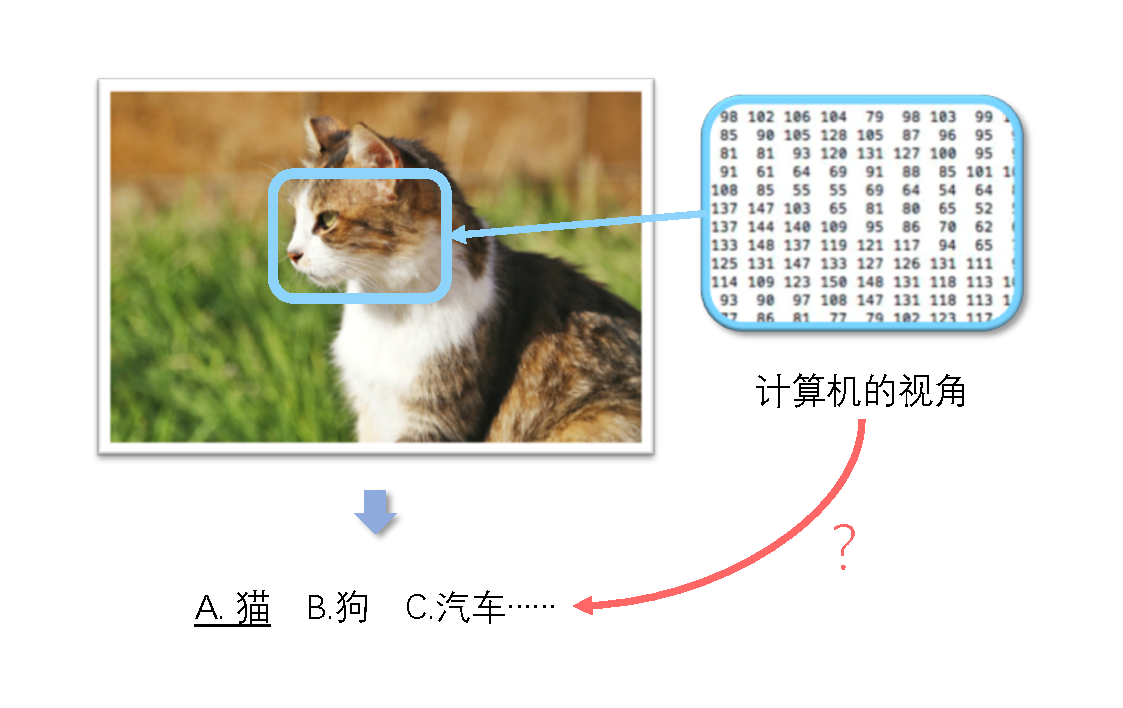
\includegraphics[width=.7\textwidth]{classify}
	\caption{图像分类问题}
	\label{fig:classify}
\end{figure}

\subsection{手工设计特征与二维深度学习}
在早期的计算机视觉研究中,人们使用了一些手工设计的方法,来提取图片和视频的局部和全局特征,并将其作为输入的一种特殊表示。比较经典的特征提取方法有
Gabor 变换\cite{gabor}、Canny 边缘检测\cite{canny}、Harris角点检测\cite{harris}、
尺度不变特征变换 (Scale-invariant Feature Transform, SIFT)\cite{sift}、
方向梯度直方图 (Histogram of Oriented Gradient, HoG)\cite{hog, hog2}、词袋模型 (Bag-of-words Model, BoW Model) \cite{bow} 等。这些经典算法得到的特征尽可能的保留了与正确结果相关的信息,同时过滤了与之无关的信息,是更加接近于输出的表示形式。
直到深度学习发展得如火如荼的今天,它们仍然在一些特定领域中被广泛应用,例如机器人的同步定位与地图构建 (Simultaneous Localization and Mapping, SLAM)\cite{slam}任务等。

然而对于不同的任务来说,我们需要的提取的信息往往是不同的。上述通用方法提取到的特征通常与具体问题无关,没有充分挖掘问题与输入数据的规律与特点。深度学习就是解决此不足的方法之一,也是近年来的研究热点。它首先将输入转化成一些简单的特征,然后再进一步将其转化为一系列相对复杂的特征,由浅入深、循序渐进地将输入一步步变换为正确输出。与早期研究不同,这些特征是通过机器自动学习得到的,而非手工设计得到的。

因为需要通过机器从已有的训练数据中自动学习到特征,所以深度学习算法是一种数据驱动的算法,而且其成败与数据的优劣密不可分。随着社会数字化的推广与互联网技术的普及,海量的互联网数据变得容易收集与管理,深度学习数据集的准备任务也不再高不可攀。近年来,我们也看到了不少优秀的大规模数据集,如 ImageNet\cite{imagenet}、Microsoft Common Objects in Context (COCO) \cite{coco}等,它们的出现极大地推动了深度学习的发展进程。



\begin{figure}[H]
	\centering
	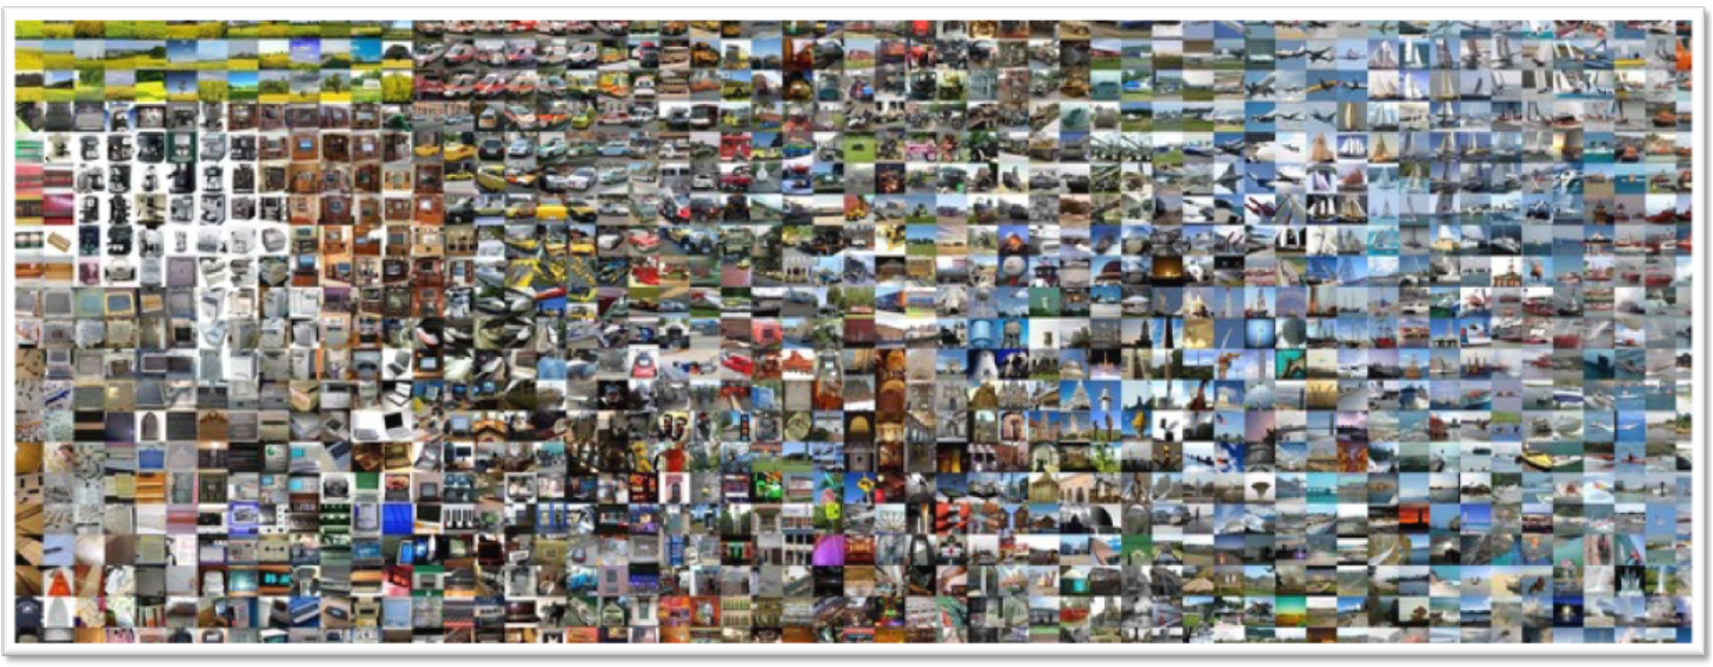
\includegraphics[width=.95\textwidth]{imagenet}
	\caption{ImageNet 数据集 \cite{imagenet}}
\end{figure}

模型的结构也是制约深度学习成败的关键因素。为了进一步提升深度学习算法的准确率,相当多的优秀工作涌现了出来,例如 AlexNet\cite{alexnet}, VGG\cite{vgg}, GoogLeNet\cite{googlenet}, ResNet\cite{resnet} 等。这些工作提出的模型在最大的对象识别比赛——ImageNet 大型视觉识别挑战 (ImageNet Large Scale Visual Recognition Competition, ILSVRC) 上一次又一次的刷新着记录,向我们展示着深度学习的强大威力。此外,不仅仅是图像分类,这些模型的思想还被用于解决物体检测\cite{rcnn, fastrcnn, fasterrcnn, ssd, yolo}、图像分割\cite{maskrcnn, fcn}、图像生成
\cite{gan, dcgan, wgan, wgangp, lsgan, began, pggan, sngan, cvaegan}等其他问题,并取得了相当可观的结果。

\begin{figure}[h]
	\centering%
	\subcaptionbox{物体检测与图像分割\cite{maskrcnn}}
	{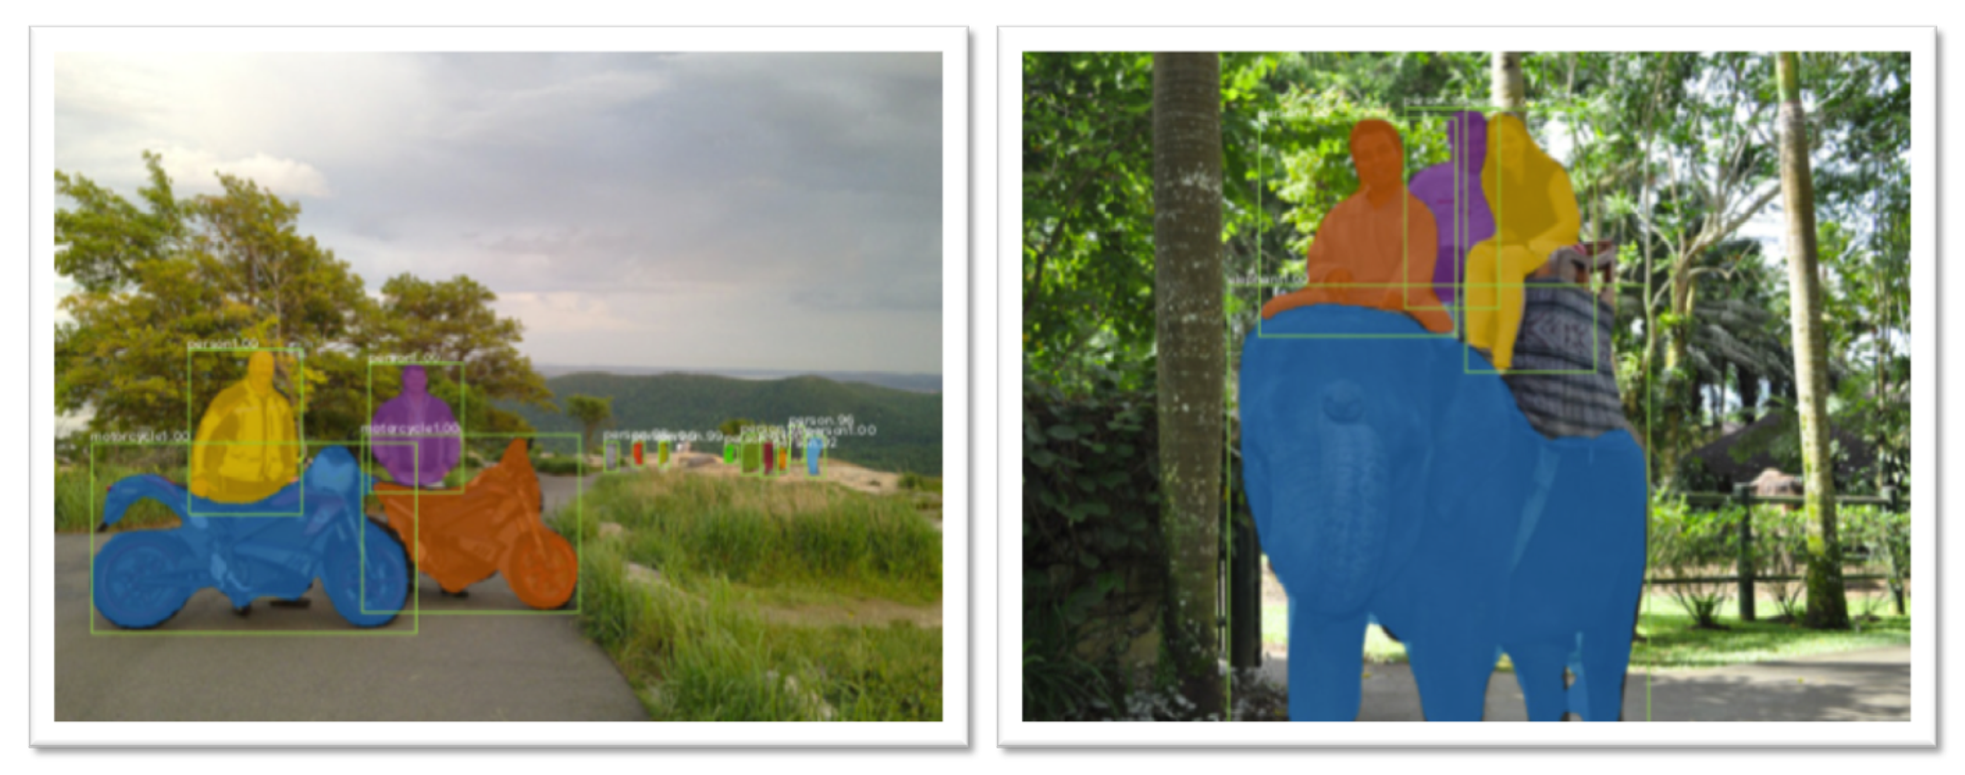
\includegraphics[width=.45\textwidth]{maskrcnn}}%
	\hspace{2em}%
	\subcaptionbox{图像生成\cite{cvaegan}\label{fig:2dgen}}
	{\includegraphics[width=.45\textwidth]{CVAE-GAN}}
	\caption{深度学习在众多问题上都取得了突破性的进展}
\end{figure}

\subsection{三维深度学习}

尽管计算机视觉在深度学习的帮助下取得了里程碑式的成果,遗憾的是它们却基本上服务于平面图像与视频等二维数据。

众所周知,
我们生活在一个三维的世界,每天都不可避免地需要与三维模型接触。而在机器人定位、虚拟现实、医学图像处理等特定任务中,
三维数据%相比于传统的二位数据,
更是占据了举足轻重的地位。因此,让计算机学会认识、理解与分析三维物体,同样是计算机视觉中的重要课题之一。我们将使用深度学习解决上述问题的方法统称为三维深度学习,以示与上节中二维深度学习的区别。

对于三维深度学习的研究,我们目前才刚刚起步。
%笔者认为,
我们认为,
阻碍三维深度学习发展的因素有三点。




首先,早期研究的三维数据规模远不如二维数据。众所周知,三维数据通常由传感器采集或者由艺术师设计。由于人力物力等客观因素的限制,能够被收集到的三维数据屈指可数。
% 深度学习等数据驱动算法的表现也必将受限于数据的规模。
这也成为了深度学习等数据驱动算法的主要瓶颈之一。

在互联网还没有普及的时代,人们曾通过三维扫描仪器和数学建模等方法,制作了 Stanford Bunny 兔子和 Utah 茶壶等经典模型。如同程序设计教程中的 \texttt{"Hello World"} 例程一样,如今它们也成为了计算机图形学中标准测试模型。
对于计算机图形学的渲染任务来说,因为其重点研究对象,如渲染方程\cite{renderequ}与双向反射分布函数 (Bidirectional Reflectance Distribution Function, BRDF)\cite{phong, blinnphong} 等,对需要被渲染的模型没有任何假设,具有一般性和通用性,因此少量标准模型的提出已经足够学科自身的发展。相反的,三维深度学习中的大部分问题却高度依赖于待处理三维模型的统计信息和分布规律,而这不可能从两个模型中直接得到。因此,它们并不能对三维深度学习带来实质性的帮助。
% 更不可能将它们作为深度学习算法的训练数据集,以训练出有效的模型解决实际的问题。


\begin{figure}[h]
	\centering%
	\subcaptionbox{Stanford Bunny 兔子}
	{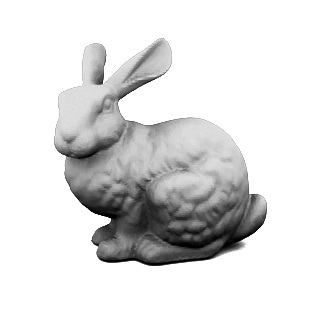
\includegraphics[width=.3\textwidth]{bunny}}%
	\hspace{2em}%
	\subcaptionbox{Utah 茶壶}
	{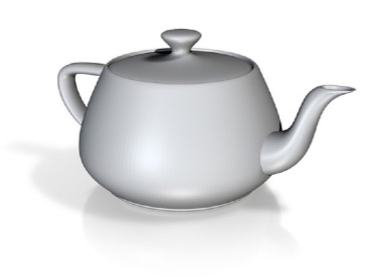
\includegraphics[width=.3\textwidth]{utah}}
	\caption{人们在早期使用的三维模型}
\end{figure}


“巧妇难为无米炊”,缺少必要训练数据,再强大的深度学习算法也无用武之地。随着互联网的普及,Princeton Shape Benchmark 数据集\cite{princetonShapeBenchmark}应运而生,极大的丰富了科研人员可用的模型数据。此数据集 包括了约 \numprint{1814} 个三维模型,分为 92 个大类。与 Stanford Bunny 兔子和 Utah 茶壶相比,虽然它在数据规模上确实有了一定的提升,但这对于深度学习所需的庞大数据量而言只是杯水车薪。它不足以让深度学习算法从中充分地挖掘出三维模型的内在规律,也不能让深度学习在相关任务中充分发挥其强大潜力。

\begin{figure}[H]
	\centering
	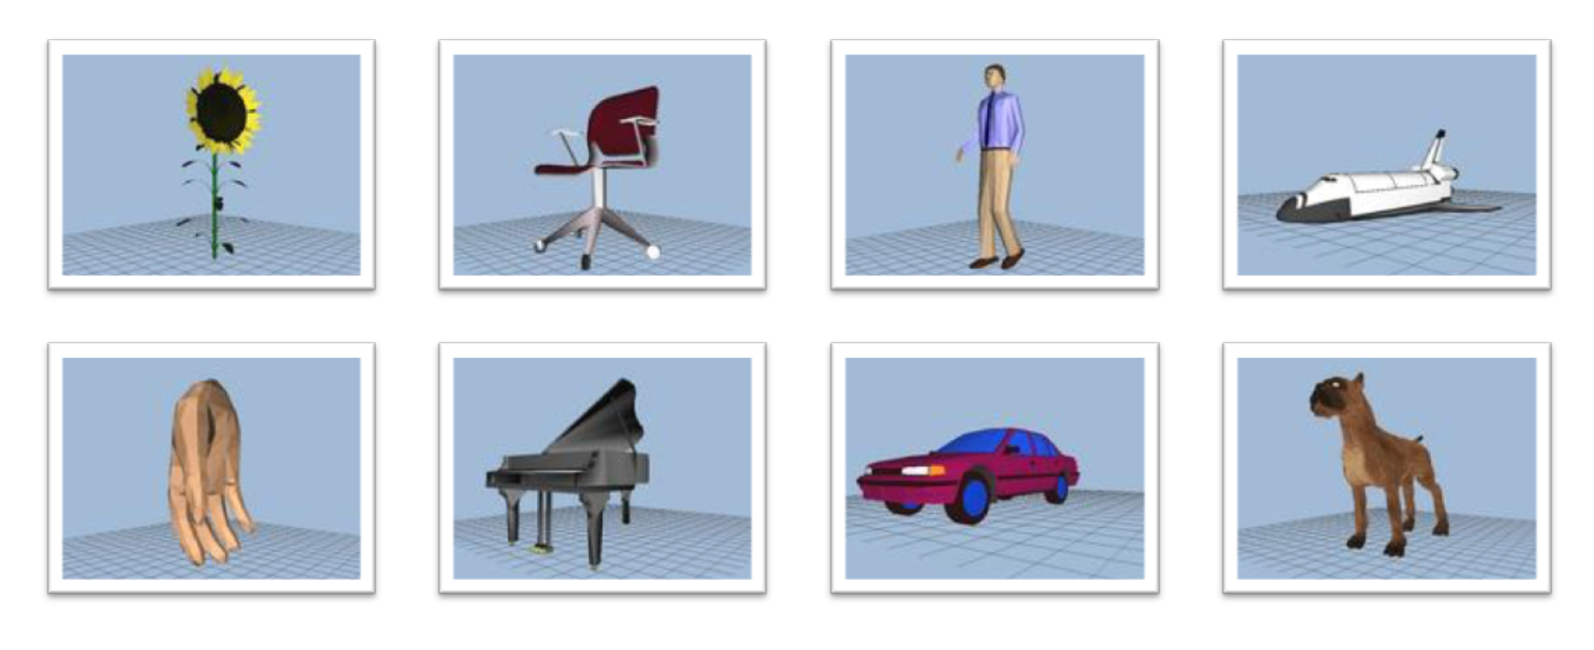
\includegraphics[width=.83\textwidth]{princeton}
	\caption{Princeton Shape Benchmark 数据集\cite{princetonShapeBenchmark}}
\end{figure}

随着计算机辅助设计 (Computer Aided Design, CAD) 系统的增强以及三维扫描设备的进一步发展,
近年来能在网络上收集到的三维模型规模有了可观的提升。
众多的三维模型仓库也不断地在互联网平台上涌现,如 Google Sketchup, 3D Houseware, Clara.io, Sketchfab 等。这些仓库均能提供至少数以万计的三维模型,让三维深度学习不再因为训练数据的短缺而止步不前。后来,人们对这些数据进行了进一步的整理和预处理,提出了 ShapeNet 数据集\cite{shapenet}。它与早期的数据集相比,规模更大,内容更丰富,共包含了 \numprint{51300} 个模型,分为 \numprint{55} 个大类。这很大程度地简化了三维深度学习的数据收集工作,为三维深度学习的发展做好了铺垫与准备。


\begin{figure}[H]
	\centering
	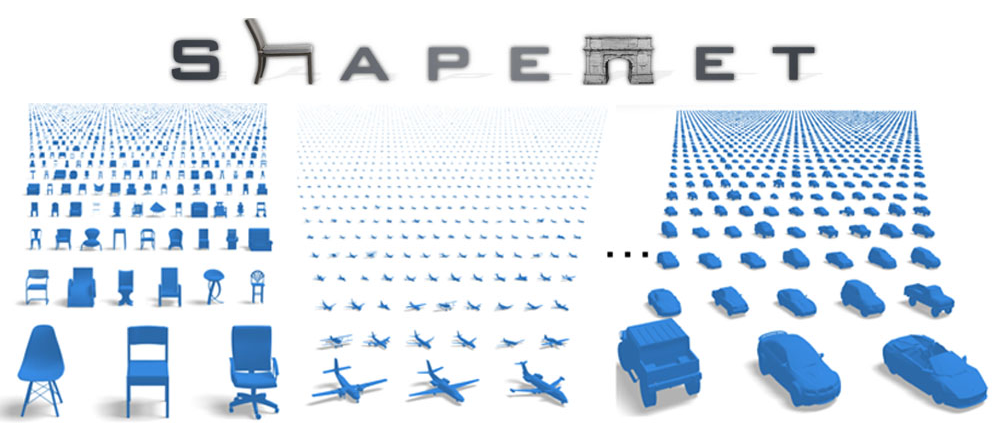
\includegraphics[width=.95\textwidth]{shapenet}
	\caption{ShapeNet 数据集\cite{shapenet}}
\end{figure}



% 另一个制约三维深度学习的因素是模型的表示方式
数据集规模并不是三维深度学习的唯一瓶颈,事实上,三维模型的表示方式同样制约着三维深度学习的发展。目前,三维模型的表示方式没有统一的规范。实际上,不同的表示方式也没有优劣之分,它们都可以在特定的需求和应用场景下发挥着无法替代的作用。
例如,将生成的三维模型通过光线追踪算法进行渲染时,我们通常需要提供模型的三角面片而非点云,因为后者不能提供法向等关键信息;而分析三维扫描设备获取的模型信息时,我们通常使用点云而非三角面片,因为后者并不是传感器采集到的原始数据。

三维模型表示的多样性也使得三维深度学习分化为了许多不同的流派。目前,三维深度学习中常见的表示方式有五种:多视角图像\cite{mvcnn1, mvcnn2, mvcnn3}、体素\cite{3dcnn, fpnn, octnet, ocnn, 3dr2n2, octgen}、三角面片\cite{surfnet, surfacecnn, syncspeccnn}、点云\cite{pointnet, pointnet2, kdnet, pointcnn, pointsetgen}以及基于 CAD 原语的参数化表示\cite{volumetricprimitives, grass}
%,如图 \ref{fig:rep} 所示
。其中,前两者是规则型的表示,所有数据都以张量的形式有规则地排列,就像图片和视频一样,故二维深度学习中的思想和算法能够直接应用于这类形式的数据;后三者是非规则型的表示,不能与已知的数据形式类比,也没有二维深度学习的算法能直接处理。目前,非规则型的表示成为了当今三维深度学习的重点研究方向。

\begin{figure}[h]
	\centering%
	\subcaptionbox{多视角图像\cite{mvcnn1}}
	{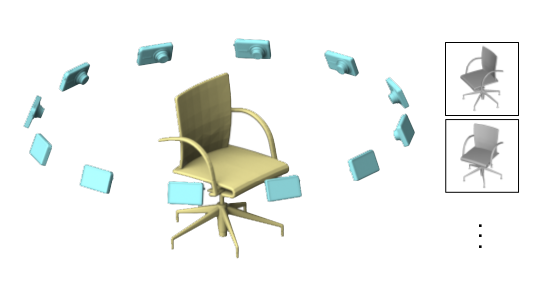
\includegraphics[height=3.4cm]{mv}}%
	\hspace{1em}%
	\subcaptionbox{体素\cite{octgen}}
	{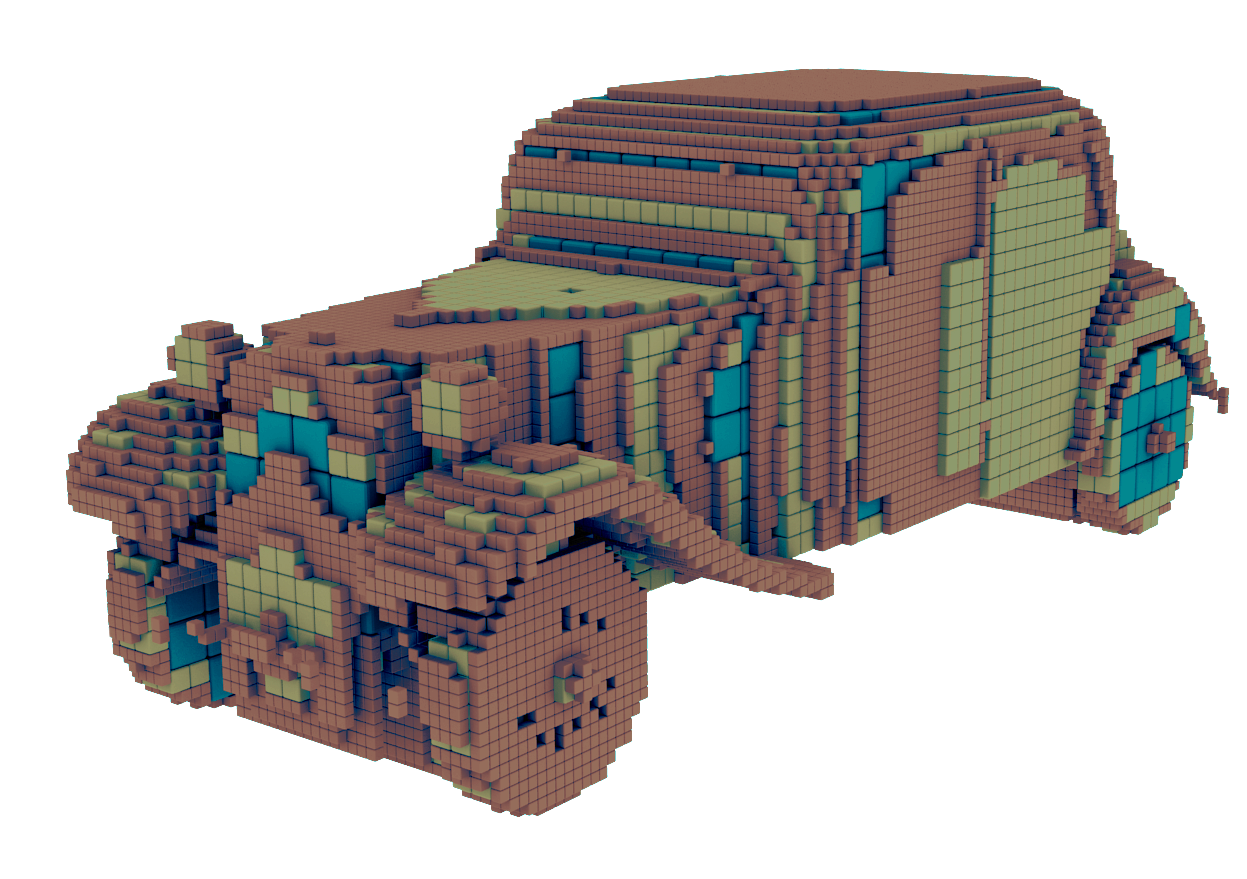
\includegraphics[height=3.4cm]{vox}}%
	\\
	\vskip1.5em
	\subcaptionbox{三角面片\cite{syncspeccnn}}
	{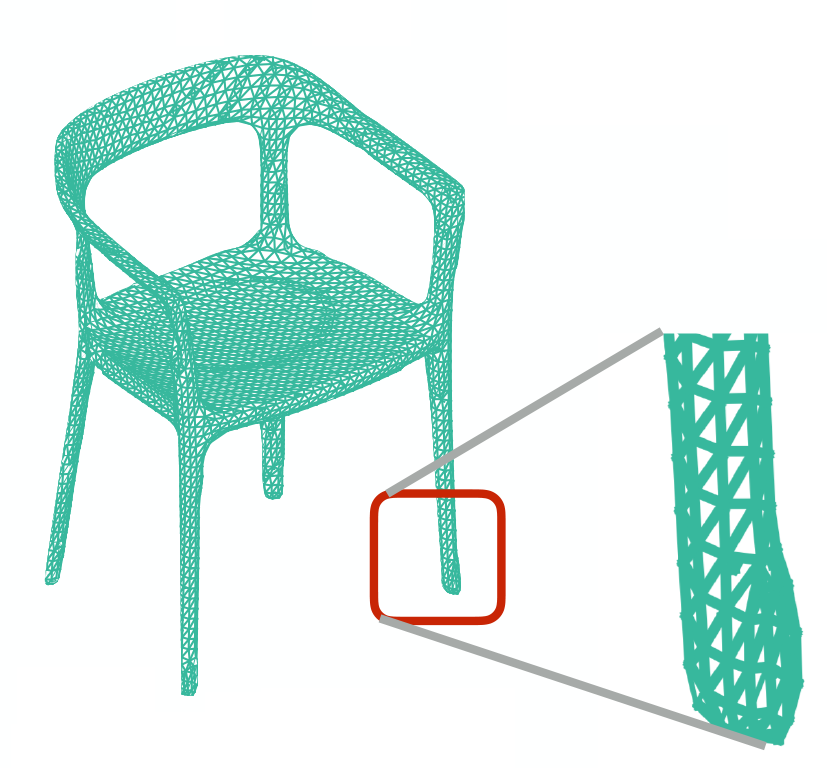
\includegraphics[height=3.4cm]{pm}}%
	\hspace{1em}
	\subcaptionbox{点云\cite{pointsetgen}}
	{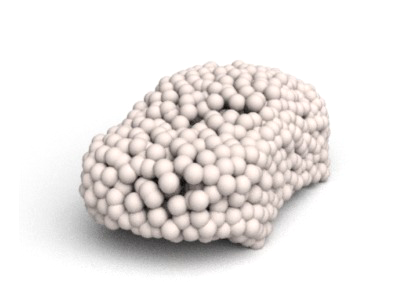
\includegraphics[height=3.4cm]{pc}}%
	\hspace{1em}
	\subcaptionbox{CAD 原语\cite{grass}}
	{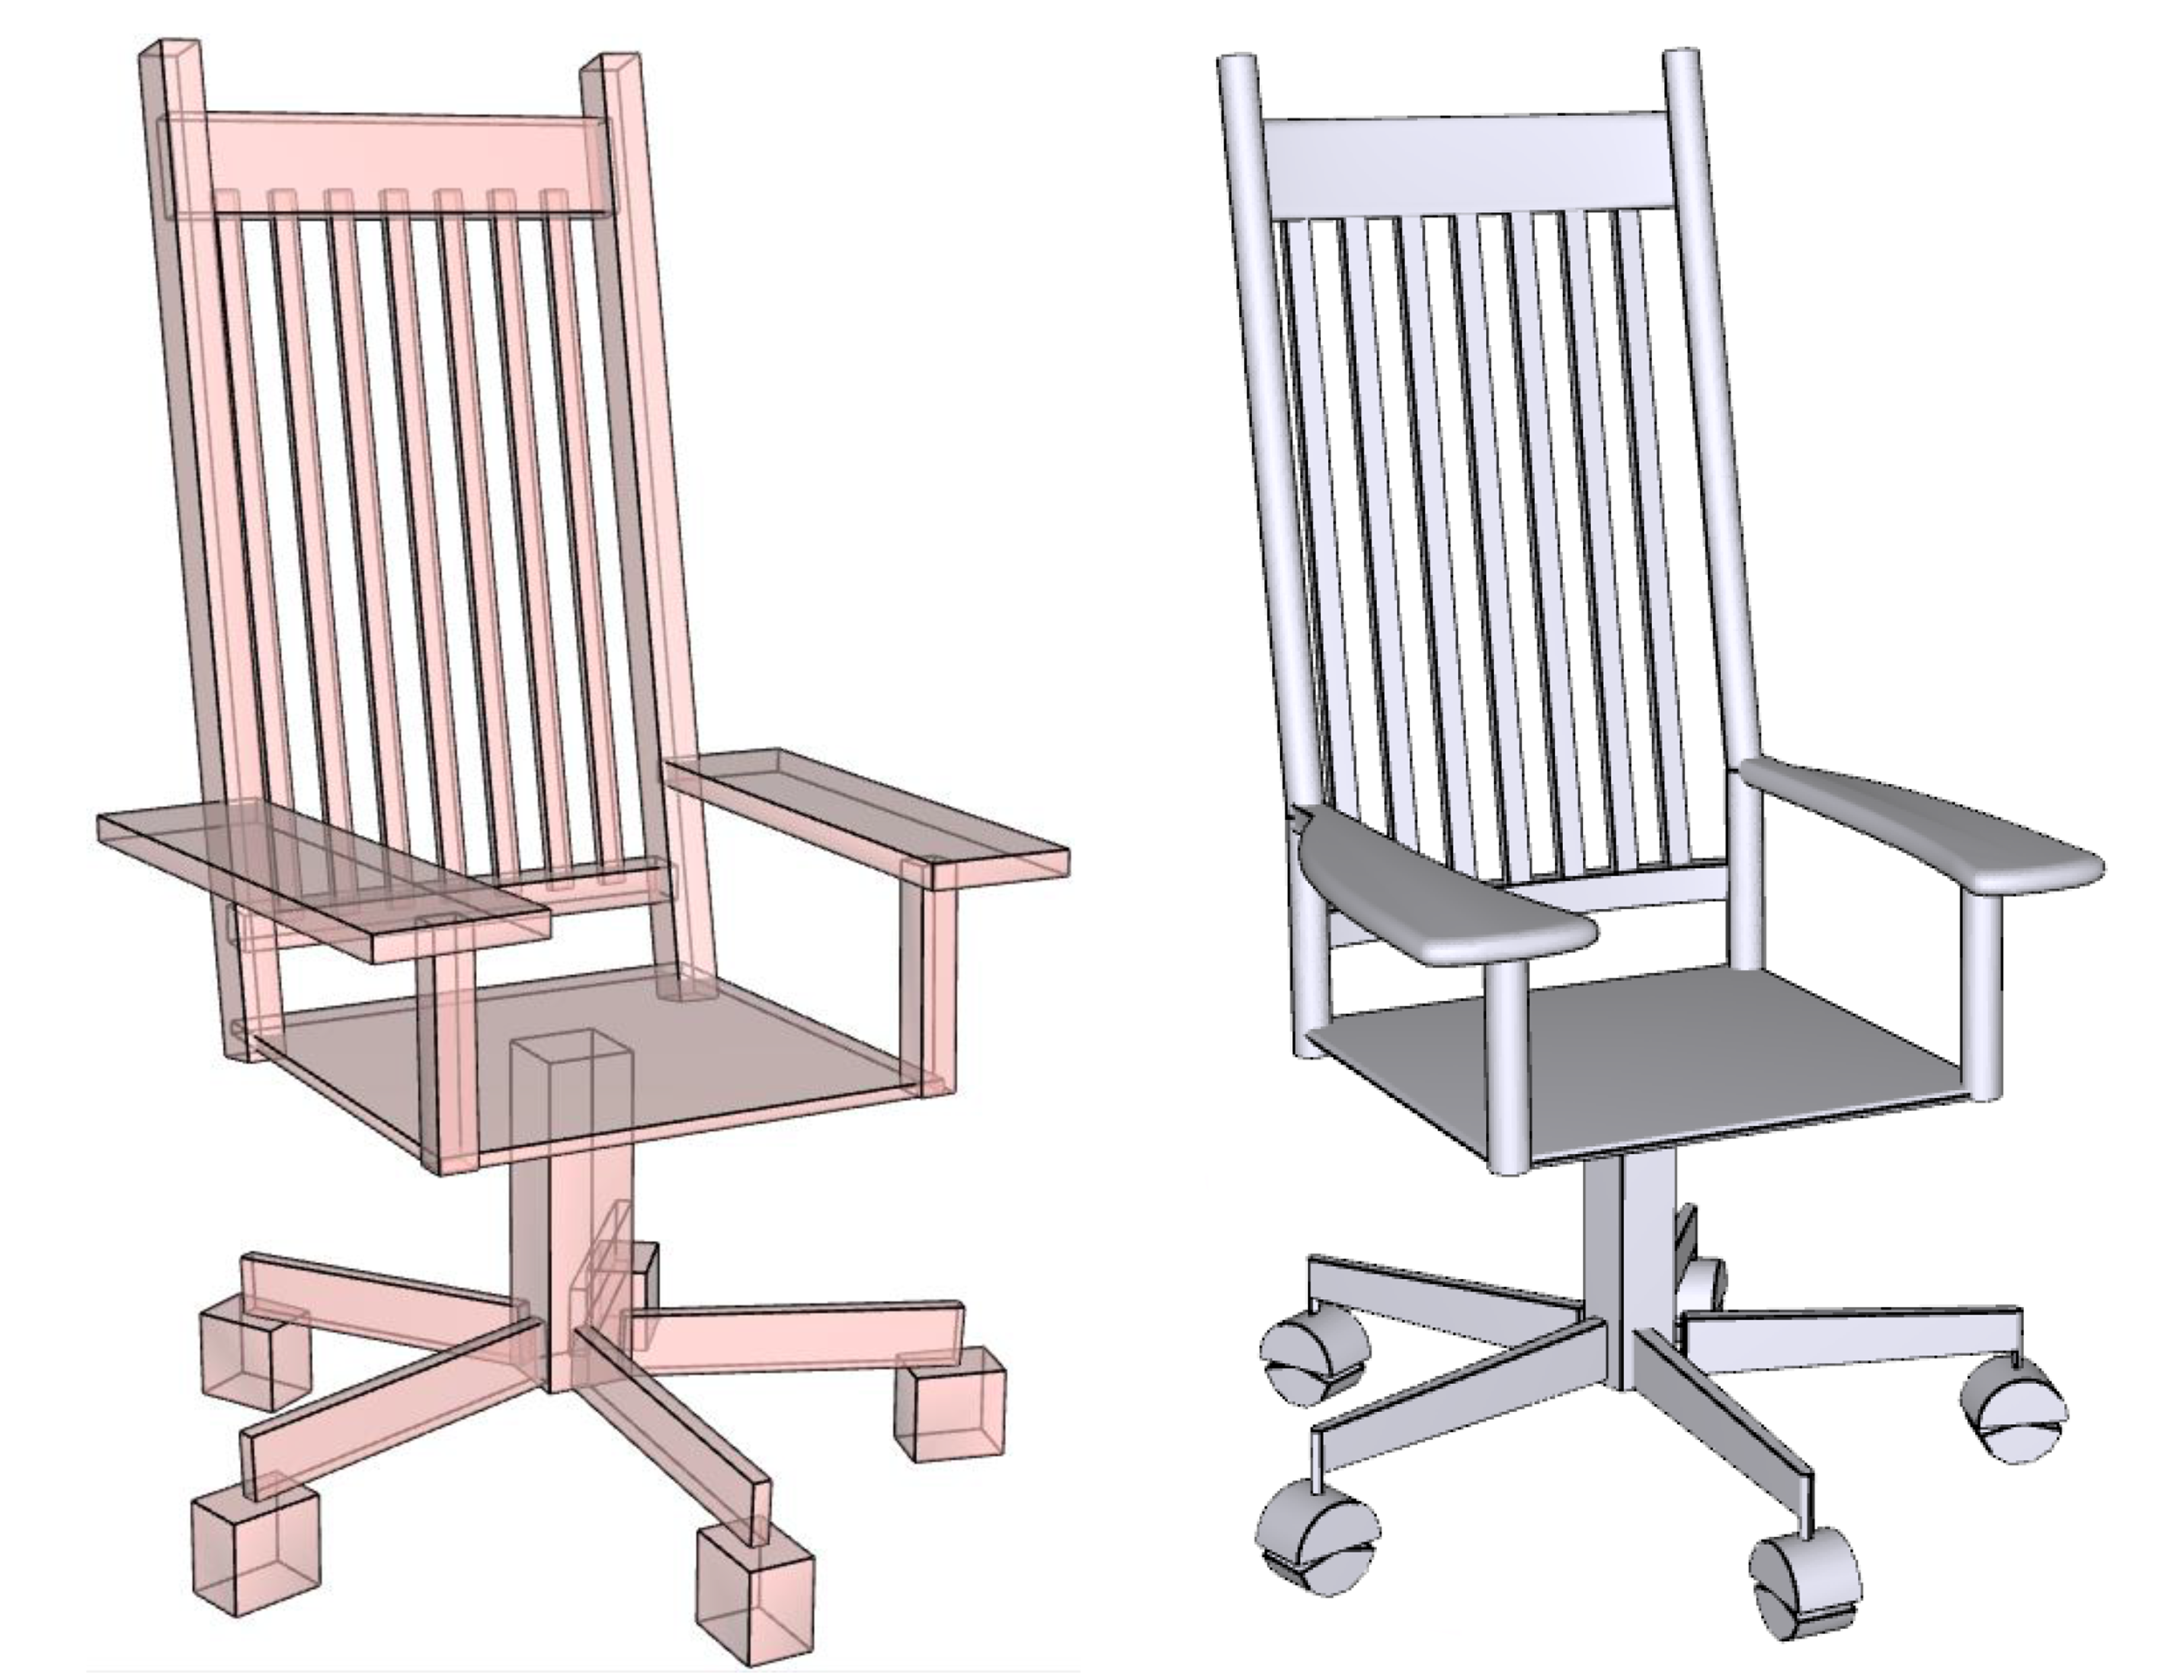
\includegraphics[height=3.4cm]{cad}}
	\caption{三维深度学习中常见的五种表示方式}
	\label{fig:rep}
\end{figure}


最后一个制约三维深度学习的因素是三维数据自身的大小。在表现形式上,三维数据比图像等二维数据多了一维,因此要直接借用二维深度学习的思路达到与之等效的结果,计算量至少需要增长一个数量级。这通常是客观条件所不允许的。

以体素表示为为例,经典的 AlexNet\cite{alexnet} 使用了尺寸为 $224 \times 224$ 的 RGB 图像作为输入,如果把它直接扩展为 $224 \times 224 \times 224$ 三维体素表示,则硬件需求和计算时间至少要增加两百倍。在时间和硬件资源的双重限制下,我们不得不作出折衷和妥协。例如, 3DShapeNets\cite{3dcnn} 使用了一个 $30 \times 30 \times 30$ 的三维体素表示作为输入,这虽然与 AlexNet 的计算量在数量级上基本持平($224^2 = \numprint{50176} \approx \numprint{27000} = 30^3$),但低分辨率的采样操作使得三维模型的质量大打折扣。

值得庆幸的是,并不是所有的表示方式都像体素一样庞大。
点云就是这样一种简约的表示方式,其本质是在三维模型的二维表面上进行采样,形式上记录着三维的信息,但实则只有二维的数据量。虽然没有经典的二维深度学习方法可以直接借鉴,但只要设计好合理的方式进行处理,点云这种新兴的表示方式必将为三维深度学习指出一条崭新的出路。

本文的研究正是从点云表示出发,探索其能在多大程度上改善三维深度学习的表现。

%\begin{figure}[h]
%  \centering%
%  \subcaptionbox{三角面片表示}
%    {\includegraphics[width=.4\textwidth]{utah-mesh}}%
%  \hspace{3em}%
%  \subcaptionbox{体素表示}
%    {\includegraphics[width=.4\textwidth]{utah-vox}}
%  \caption{低分辨率体素化表示}
%\end{figure}

%此外,这样的妥协还会


\section{研究现状}

三维深度学习中研究的问题是二维深度学习的继承和拓展,其外延不仅包括二维深度学习中的常见问题,如分类\cite{pointnet}、检测\cite{frustumpointnet}、分割\cite{pointnet}、生成\cite{latentpc}等,还包括一些三维深度学习中独有的问题,如视角恢复\cite{rendercnn},三维重建\cite{pointsetgen},形状补全\cite{shapecomplete}等。在实际应用中,无论被处理的三维模型是以何种表达形式呈现的,求解这些问题的需求是客观存在的。
因此,各种流派的三维深度学习可以按照问题目标被进一步细分。

目前,点云相关的三维深度学习研究进展得如火如荼。针对点云的各种处理需求,人们提出了多种不同的模型与算法来灵活应对和处理。限于篇幅,此处列举并简要介绍与本文相关性最大的三个工作。各工作的具体细节,我们将在第 \ref{cha:3d_deep_learning}、\ref{cha:gen}  章中予以详细说明。

\subsection{基于图片的三维点云重建}

PointSetGen\cite{pointsetgen} 是第一个将点云引入三维深度学习的工作,开创了历史先河。此工作的核心目标是希望从输入的单张 RGBA 图像中直接重建出物体的三维结构,并以点云的形式输出结果,如图 \ref{fig:pointsetgen} 所示。


\begin{figure}[h]
	\centering%
	{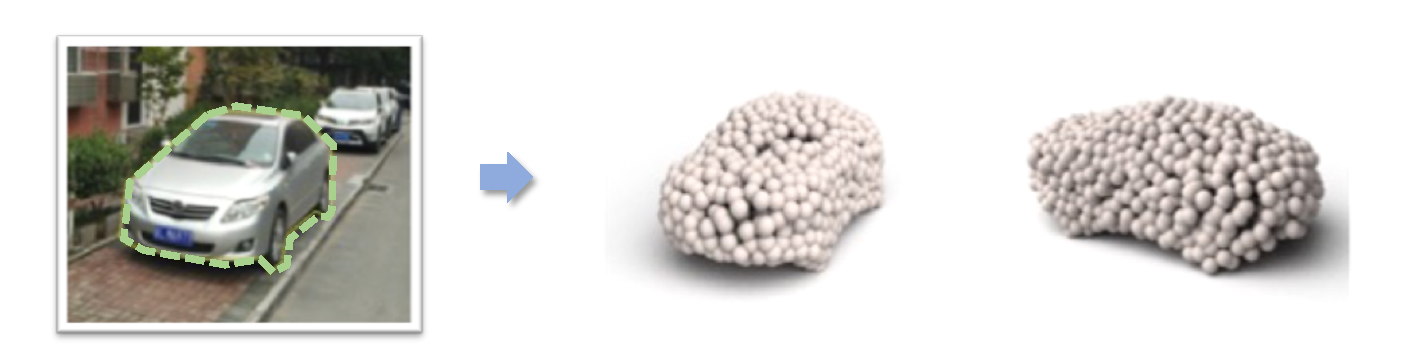
\includegraphics[width=.95\textwidth]{pointsetgen}}
	\caption{基于图片的三维点云重建:PointSetGen\cite{pointsetgen}}
	\label{fig:pointsetgen}
\end{figure}

此工作最大的贡献在于提出了点集 $S = \{(\bm p_i)\}_{i=0}^{N - 1}$ 之间的度量方案——Chamfer 距离 (Chamfer Distance, CD) 和 推土机距离 (Earth Mover's Distance, EMD):
\begin{align}
	\DCD{S_1}{S_2}  & =
	\sum_{\bm p \in S_1} 􏰘\min_{\bm q \in S_2} \Norm*{\bm p - \bm q}^2 +
	\sum_{\bm q \in S_2} 􏰘\min_{\bm p \in S_1} \Norm*{\bm p - \bm q}^2 \label{eq:cd} \\
	\DEMD{S_1}{S_2} & =
	\min_{\text{双射} \phi:\, S_1 \to S_2} \sum_{\bm p \in S_1} \Norm*{\bm p - \phi(\bm p)}_2
	\label{eq:emd}
\end{align}
利用这两个度量,我们很容易定义模型输出与真实情况的差距,即损失函数。
只要
%通过
最小化上述损失函数,我们就可以得到高质量的模型,从而解决问题。

\subsection{点云数据的分类与分割}
PointNet \cite{pointnet} %的提出
主要
解决了点云数据的分类与分割问题,如图 \ref{fig:pointnet} 所示。

\begin{figure}[h]
	\centering%
	{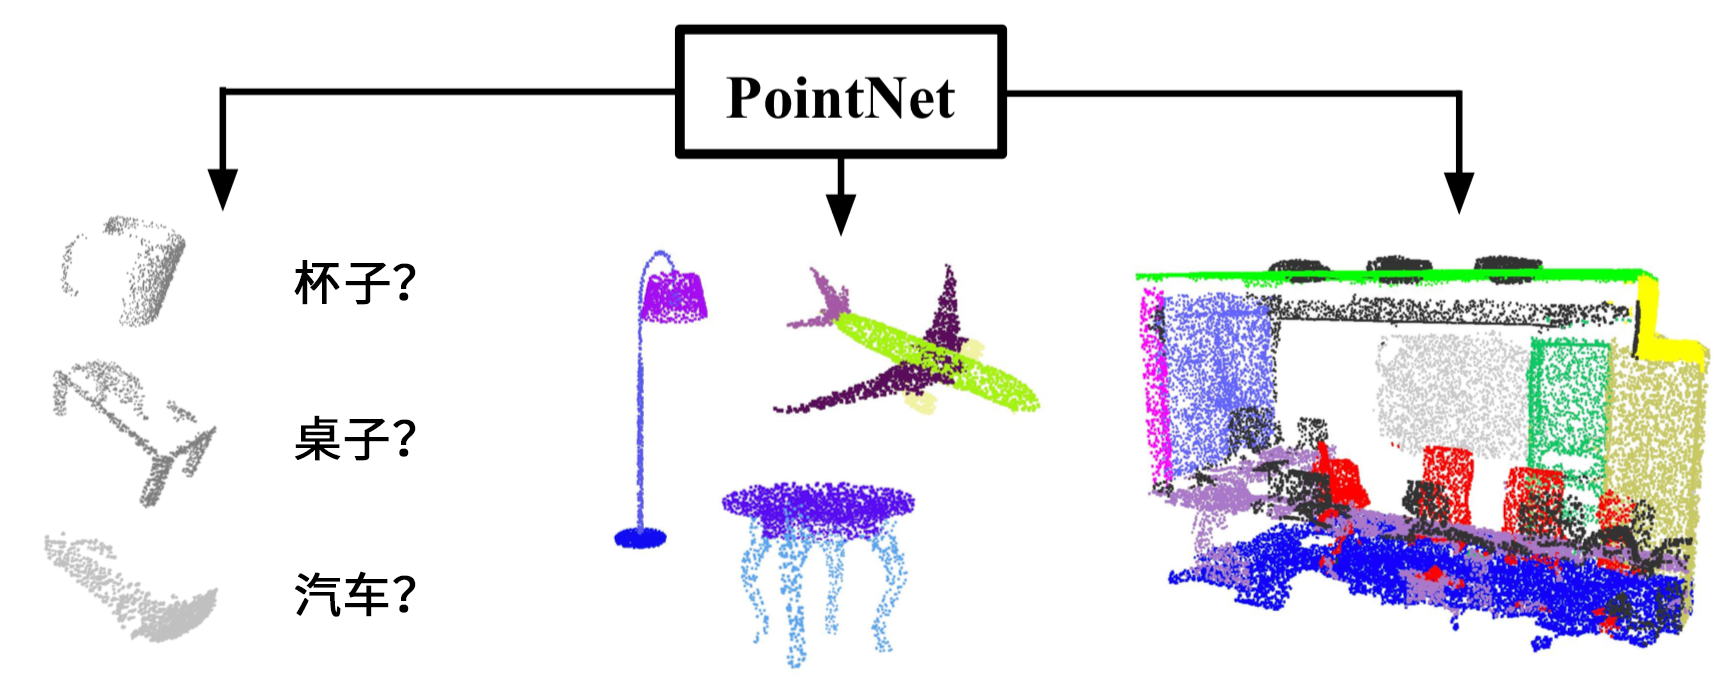
\includegraphics[width=.95\textwidth]{pointnet}}
	\caption{点云数据的分类与分割:PointNet \cite{pointnet}}
	\label{fig:pointnet}
\end{figure}

此工作从点集的排列不变性入手,提出了使用对称函数来处理点云输入的观点。

对称函数是一类数学函数,其输出不随输入变量的排列而发生变化。例如对一组数相加、相乘、求最大值或者最小值等,都是对称函数。%而
点云的分类和分割同样是对称函数。
容易观察到,如果存在映射 $h: \mathbb{R}^3 \to \mathbb{R}^K,
	g: \underbrace{\mathbb{R}^K \times \mathbb{R}^K \times \cdots \times \mathbb{R}^K}_{N} \to \mathbb{R}^K, \gamma: \mathbb{R}^K \to \mathbb{R}$,且 $g$ 为对称函数,则映射 %$f: S \to \mathbb{R}$
\begin{align}
	f(\{\bm p_1, \ldots, \bm p_N \}) = \gamma \circ g(h(\bm p_1), \ldots, h(\bm p_N)) \label{eq:symmetric}
\end{align}
亦为对称函数。
只要把 \eqref{eq:symmetric} 作为模型架构,并
取 $g$ 为 多个向量的逐元素最大值 (Element-wise Maximum) % $g = \max$ 
等简单的对称函数,$h, \gamma$ 为一个深度神经网络,就可以近似出一个合理的模型以解决问题。


\subsection{点云数据的隐表示与自动生成模型}
近年来,深度学习的研究热点逐渐从分类问题转向了生成问题。目前最前沿的图像生成结果已经达到了以假乱真的地步,而且还在不断的提升,如图 \ref{fig:2dgen} 所示。
那么,点云生成能否做到这样的程度呢?

文献 \inlinecite{latentpc} 的工作对此做出了肯定的回答。
通过将已有的点云深度学习算法与深度生成算法相结合,我们可以生成出多样的三维模型,且达到了与图像生成相似的结果。

值得注意的是,这个算法并不是直接在已有数据集中随机抽取一个输出,而是实实在在的学习到了三维模型内在的统计规律,
并依此举一反三地生成全新的三维模型。这样的算法可以对输出结果做插值和代数操作,是
%前者
朴素算法
所不能比拟的。


% PointGAN 


\section{本文的主要工作与贡献}


% 本文的工作是对基于点云的三维深度学习的一次摸索与尝试。


%我们
本文要解决的核心任务是进一步提升点云三维重建的质量。
具体地,我们首先使用已有算法,实现了一套基于单物体单图像的三维点云重建系统。
其读取单张 RGB 图像,自动生成 mask,并以点云的形式重建并输出图中物体的三维形态。
随后,我们将已有的重建算法与图像生成任务中的经典算法进行了有机的结合,不仅提高了原算法的重建质量,而且还增强了输出的多样性,使得算法的输出结果更加真实,同时能生成出更多的模型,而不受限于仅有的输入图像。

例如,用户可以对于多张不同图片的重建结果进行加权平均,生成出介于各个模型间的一个中间形态。这在用户不容易得到目标物体图像的情况下很有意义。
值得注意的是,这并不是通过直接对输出结果进行插值实现的,而是对于隐表示进行操作的结果,因为前者这样的素朴处理方式和并不一定能生成合理的结果。

综上所述,本文的主要贡献有:
% \begin{itemize}
%   \item 提出了一套更加自动、用户友好的三维重建系统:用户不必像已有算法一样花费大量时间提供 mask 信息;
%   \item 改善了已有工作的重建质量:已有算法重建失败时,本文算法仍然能给出合理的重建结果;
%   \item 增加了模型的生成能力:%本文提出的算法
%   本工作能生成的物体并不局限于输入图像中记录的对象。
% \end{itemize}
% 本文的主要贡献有:
\begin{itemize}
	\item 提出了一套更加自动、用户友好的三维重建系统:通过整合已有技术,用户不必再花费时间提供 mask 信息;
	      % \item 提出了一套更加自动、用户友好的三维重建系统:用户不必像已有算法一样花费大量时间提供 mask 信息;
	\item 改善了已有工作的重建质量:已有算法重建失败时,本文算法仍然能给出合理的重建结果;
	\item 增加了模型的生成能力:%本文提出的算法
	      %本工作能生成的物体并不局限于输入图像中记录的对象。
	      本文算法比已有算法更灵活,可能对多个重建结果进行插值,输出结果也更丰富多样。
\end{itemize}

\section{本文的行文结构}
本文的行文结构如下:
\begin{itemize}
	\item %在
	      第 \ref{cha:intro} 章%中,我们将
	      主要介绍了与本文工作相关的历史背景和研究现状,并说明了本文工作的主要内容与贡献;
	      % 具体的,我们计算机视觉的历史由来引入,逐步介绍了计算机视觉的研究是如何从手工设计特征出发,逐步拓展到二维深度学习与三维深度学习的。随后,我们讲解了三维深度学习的难点与分类,强调了点云三维深度学习的重要意义,并以三个点云深度学习为例进行了简要介绍。最后,我们说明了本文工作的主要内容与贡献。

	\item 第 \ref{cha:3d_deep_learning}、\ref{cha:gen} 章主要介绍了已有的工作成果,是第 \ref{cha:exp}、\ref{cha:result} 章的本文工作预备与铺垫。其中:
	      \begin{itemize}
		      \item %在
		            第 \ref{cha:3d_deep_learning} 章
		            % 中,我们
		            详细讲解了点云三维深度学习及其重要工作 PointSetGen\cite{pointsetgen} 和 PointNet\cite{pointnet}。而前者 PointSetGen 则是本文主要参考以及改进的对象;
		      \item %在
		            第 \ref{cha:gen} 章%中,我们主要介绍
		            主要引入了深度生成模型,是本文工作的理论支撑;
		            % \item %在
		            % 第 \ref{c h a: g e n 3 d} 章%中,我们
		            % 主要讨论了基于点云的三维深度生成模型,证实了本文工作在实践上可行性;
	      \end{itemize}
	\item %在
	      第 \ref{cha:exp}、\ref{cha:result} 章%中,我们主要介绍
	      详细讲解并记录了本文工作的算法流程与实验结果,是全文的核心与关键;
	\item %在
	      第 \ref{cha:summ} 章%中,我们对
	      %是
	      简洁明晰地分析并总结了本文工作,指出了其意义与贡献,
	      %本文工作
	      %进行
	      %的
	      %分析与总结,
	      同时也
	      %并简要指出了
	      给出了未来可能的改进方向。

\end{itemize}








% 
% 
% 随着以及计算机硬件系统的发展,
% 计算机视觉已经取得了突飞猛进的进展。借助海量数据以及深度学习的方法,我们已经可以在图像分类、物体识别、
% 物体分割、图像生成等任务上取得相当可观的结果。
% 
% 
% 然而,对于三维物体的相关理解任务,我们才刚刚起步。首先,三维数据在表现形式上比图像等二维数据多了一维。
% 直接使用已有算法会使得计算量增长一个数量级,结果自然会受限于时间和硬件资源的限制。
% 其次,三维数据的表示形式多样。诸如点云、三角面片等不规则的表示,根本无法被已有算法直接处理。
% 最后,


\chapter{基于点云的三维深度学习}
\label{cha:3d_deep_learning}

点云本身并不是一个新概念。事实上,早期的三维激光扫描仪的原始输出正是点云。
但是,这样的仪器在当时并不普及,相关的需求也不大,因此鲜有学者对其展开深入的研究。%其服务对象通常是专业人员,而非普通大众。
而近年来,三维扫描设备得到了很大发展,甚至已经集成并嵌入到了 Kinect 和 iPhone X 等大众化产品内部,使得点云数据真正走入到人们的日常生活当中,点云三维深度学习相关的需求也呼之欲出。


\section{点云三维深度学习优劣与特点 \label{section:pcintro}}
点云具有许多优良的特性
,%使得其表现往往优于其他形式。这也
使得它成为当今三维深度学习的研究热点。

正如第 \ref{cha:intro} 章中所介绍的,点云的本质是在三维模型的二维表面上进行采样的结果。其形式上记录着三维的信息,但实则只有二维的数据量,因此是一种非常稀疏的表示。与体素和多视角图像图像相比,点云占用的空间更小,对计算资源的需求也更低。

此外,点云数据非常容易进行预处理。在二维深度学习中,数据增强是我们常使用的一个预处理技巧\cite{alexnet},例如在图像上随机切割,旋转,翻转等。这样的操作通常需要在流水线前端配置一个较为复杂的预处理程序。
但对于点云来说,简单的矩阵乘法即可完成同样的功能\cite{pointnet},而且非常容易通过现有的深度学习框架实现,并在 GPU 上高速执行。


“尺之木必有节目,寸之玉必有瑕瓋”,点云也不是十全十美的表示形式。
卷积神经网络 (Convolutional Neural Network, CNN) 的巨大成功\cite{lenet5, alexnet, vgg, googlenet, resnet},与其对局部细节的重视密不可分。在经典的卷积神经网络中,每一层中间表示的取值只于上一层附近的区域有关。由于数据是规则的,因此可以按照位置被迅速索引,高效地提取局部细节信息。%不必费除灰之力。
然而,点云数据却是无序的,因此局部细节的提取非常麻烦。在没有对各点位置进行有效索引的情况下,我们不得不遍历整个点集,效率低下。而即使借助 $k$-d 树 等数据结构实现了高效的处理,其复杂程度也远远超过了传统的情况,不便于使用 GPU 等并行计算设备进一步加速。


但是,我们应当承认,点云三维深度学习提出影响深远,意义重大。
它将不规则的几何表示与深度学习算法相结合,打破了原来深度学习只能处理规则型数据的思维定势,为我们的研究开辟了一条崭新的道路。

诚然,相对于点云而言,三角面片和基于 CAD 原语的参数化表示是三维模型更自然、更准确、更完善的表现形式。但正因为如此,它们也更复杂,更不容易被现有深度学习算法所处理。
因此,%笔者
我们认为点云是三维深度学习发展过程中一个必然的
%历史过渡
历史阶段
,是一个连接传统二维深度学习与更高级的三维深度学习之间的重要桥梁。


\section{基于图片的三维点云重建 \label{section:pointsetgen}}
本节介绍 PointSetGen\cite{pointsetgen} 工作的主要内容。
\subsection{问题描述}
PointSetGen
解决了点云的三维重建问题,是本文的主要参考对象。在这个工作中,用户需要提供一张三维物体的 RGBA 图像,即 RGB 图像与 mask 信息。 随后,算法会根据输入图像,以点云的形式重建出三维模型的完整结构,包括遮挡与不可见的部分。另外,为了简化问题,我们进一步假设生成结果中点云的点数 $N$ 为固定常数,如 $N =  \numprint{1024}$。

图 \ref{fig:pointsetgen} 是使用本算法进行重建例子。可以看到,由于遮挡等原因,输入图像中汽车的尾部并不可见,
然而这并不影响重建算法的运行。在重建结果中,汽车尾部的形状仍然清晰可见。

\subsection{模型架构}
遮挡、投影等客观因素,造成了信息的丢失,使得问题的解具有一定的多样性和不确定性。因此,此工作首先引入了一个随机变量 $\bm r \sim \NormDist(\bm 0, \bm I)$ 来刻画这样的不确定性。令输入的 RGBA 图像为 $\bm I$,输出的点云为 $S = \{(\bm p_i)\}_{i=0}^{N - 1}$,则此工作的基本流程与结构可用下式表示:
\begin{align}
	S = G(\bm I, \bm r; \bm  \theta)
\end{align}
其中 $G$ 是网络架构,$ \bm \theta$ 是需要学习出的网络参数。

基本版 PointSetGen 的网络架构 $G_{\text{vanilla}}$ 如图 \ref{fig:vanillapointsetgen} 所示。它首先通过二维深度学习中经典的卷积神经网络,将输入图像 $\bm I$ 映射为一个隐向量。随后,将计算出的隐向量通过一套全连接网络,便可以回归出最终的输出点云。尽管这个网络很简单,它的效果却出乎意料的好。
\begin{figure}[h]
	\centering%
	\subcaptionbox{基本版 PointSetGen 的网络架构 $G_{\text{vanilla}}$\label{fig:vanillapointsetgen}}
	{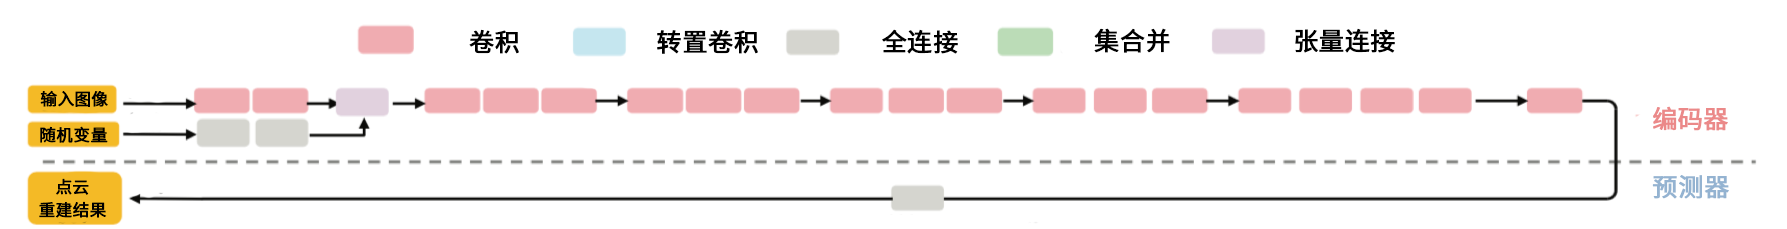
\includegraphics[width=.95\textwidth]{vanillapointsetgen}}
	\\

	\subcaptionbox{双分支版 PointSetGen 的网络架构 $G_{\text{two\_branch}}$\label{fig:tbpointsetgen}}
	{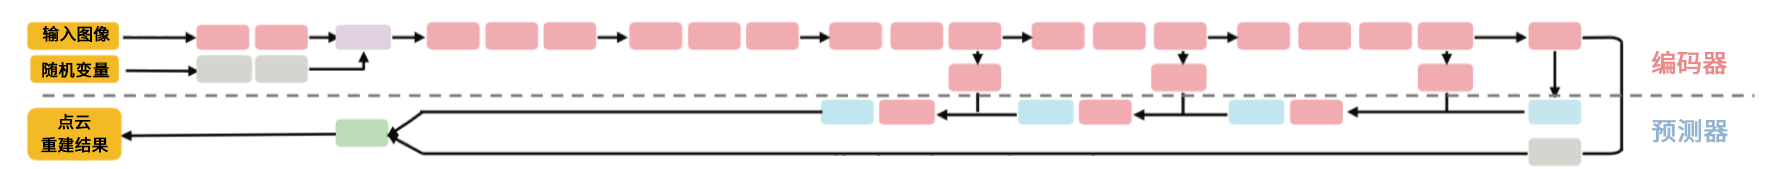
\includegraphics[width=.95\textwidth]{tbpointsetgen}}
	\\

	\subcaptionbox{Hourglass 版 PointSetGen 的网络架构 $G_{\text{hourglass}}$\label{fig:hpointsetgen}}
	{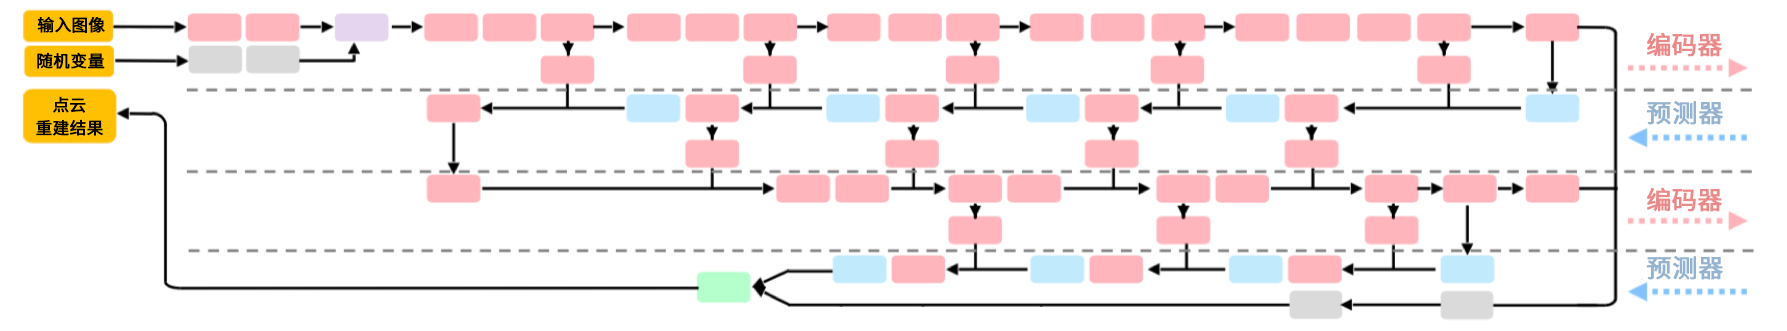
\includegraphics[width=.95\textwidth]{hpointsetgen}}
	\\

	\caption{PointSetGen\cite{pointsetgen} 的网络架构 $G$}
\end{figure}


在基本版的网络架构 $G_{\text{vanilla}}$ 中,各个点的输出是互相独立地被预测出来的,并没有任何相关性。然而在真实世界中,各点之间往往是有相关性的,如构成一个平滑表面、棱、角等。为了更好的刻画这样的相关性,双分支版本 $G_{\text{two\_branch}}$ 对全连接网络进行了调整,用一个转置卷积网络 和 更小的全连接网络进行了替换,其中前者提供 $3/4$ 的点,后者提供 $1/4$ 的点。两者组合起来便形成了最终的输出,如图 \ref{fig:tbpointsetgen} 所示。与基本版相比,双分支版的效果略有提升。



Hourglass 版本的网络架构 $G_{\text{hourglass}}$ 在已有基础上进一步提升。通过多层卷积和转置卷积操作,局部和全局的特征得到了充分的挖掘,如图 \ref{fig:hpointsetgen} 所示。其表现结果比基本版和双分支版都略有提升。


\subsection{制定衡量模型优劣的标准}
要衡量模型的优劣,并依照这个标准训练出好的模型,一个合理的损失函数是必不可少的。
% 本文
此工作
的最大贡献就是提出了两个损失函数的候选方案——Chamfer 距离 (Chamfer Distance, CD) 和 推土机距离 (Earth Mover's Distance, EMD),我们在第 \ref{cha:intro} 章中已经有所介绍:
\begin{align}
	\DCD{S_1}{S_2}  & =
	\sum_{\bm p \in S_1} 􏰘\min_{\bm q \in S_2} \Norm*{\bm p - \bm q}^2 +
	\sum_{\bm q \in S_2} 􏰘\min_{\bm p \in S_1} \Norm*{\bm p - \bm q}^2 \tag*{\ref{eq:cd}} \\
	\DEMD{S_1}{S_2} & =
	\min_{\text{双射} \phi:\, S_1 \to S_2} \sum_{\bm p \in S_1} \Norm*{\bm p - \phi(\bm p)}_2
	\tag*{\ref{eq:emd}}
\end{align}

% 设真实的结果应为 $S_{\text{gt}}$,则通过最小化 $\DCD{ S_{\text{gt}} }{S}$ 或 $\DEMD{ S_{\text{gt}} }{S}$,我们就可以得到一个合理的模型 $G(\cdot, r; \theta)$,从而解决问题。

虽然 Chamfer 距离 \eqref{eq:cd} 的求解是平凡的,但推土机距离 \eqref{eq:emd} 的值并不容易高效求得。简单分析可知,计算 \eqref{eq:emd} 等价于求解一个二分图最小权匹配的问题。能直接使用的经典算法如 %Edmonds–Karp
Kuhn-Munkres 等,至少需要 $\mathcal{O}{(N^3)}$ 的计算时间,而且很难并行化,不能发挥 GPU 的强大威力。鉴于此,这个工作进一步引入了一个近似算法实现 \eqref{eq:emd}的估算,并给出了基于 CUDA 语言的实现。限于篇幅,此处不再展开介绍近似算法的流程。

\subsection{训练模型}
由于引入了随机噪声 $\bm r \sim \NormDist(\bm 0, \bm I)$,直接使用传统的深度学习算法训练是不可取的,因为这样不能保证 $\bm r$ 能刻画出遮挡、投影等客观因素带来的多样性和不确定性。

对此,这个工作中提出了最小 $n$ 损失函数 (Min-of-N loss, MoN loss) 和 VAE 两种训练方式。使用最小 $n$ 损失训练即最小化下式:
\begin{align}
	\Loss(\bm \theta) = \sum_k
	\min_{\substack{\bm r_j \sim \NormDist(\bm 0, \bm I) \\  1 \le j \le n}}
	\DCDEMD{    G(I_k, \bm r_j; \bm \theta)    }{   S_k^{\text{gt}}   }
\end{align}
其中 $k$ 是训练数据的编号,$S_k^{\text{gt}}$ 是第 $k$ 号模型的真实点云。
而 VAE 的训练方式我们将在第 \ref{section:vae} 节中进一步展开介绍。

\subsection{训练数据集的准备 \label{section:pointsetgenpre}}
虽然我们目前已经有了充足的二维图像\cite{imagenet}和三维模型\cite{shapenet}的数据集,但这两者并没有直接的对应关系。
%在本问题里,
而在此工作中,输入图像 $I$ 与真实点云 $S^{\text{gt}}$ 是严格对应的。
如果找不到成对的二维图像和三维模型数据,我们就不能有效地%的对模型
进行训练。

在第 \ref{cha:intro} 章中,我们简要的介绍了计算机视觉与计算机图形学的历史背景与研究重点。
有趣的是,这两个学科研究的问题恰好为互逆的关系。

在计算机图形学中,通常用户会提供模型、材质、纹理、光照、摄像机视角等参数,希望计算机能尽可能自动地绘制出此场景。而在计算机视觉中,用户往往会提供一张真实拍摄的图片,并希望计算机反推出图像中的模型、材质、纹理、光照、摄像机视角等。
因此,我们能否借助图形学的手段,来完成训练数据的收集呢?

早期的 RenderForCNN \cite{rendercnn} 工作就提出了这样一个创造性的想法——通过渲染已有的三维模型,就可以得到用于训练的二维图像数据。这个工作向我们
%展示了,
证实:即使是使用计算机渲染出的图片进行训练,测试时我们仍然可以在现实生活中拍摄的图片上取得较好的结果。本节所介绍的 PointSetGen 也使用了同样的方法,完成了数据集的准备工作。


\subsection{改进方向}
%笔者
我们
认为,作为点云三维深度学习的鼻祖,此工作有非常多的亮点值得我们学习与参考,如 Chamfer 距离和推土机距离的提出,
最小 $n$ 损失函数的建立等。但
它
作为点云三维深度学习的早期工作,%此工作也难免有一定的不足。
难免会有一定的不足之处,
例如:
\begin{itemize}
	\item 此工作需要用户提供 mask 信息:用户体验差;另外
	\item 此工作对于新数据的泛化能力不强:对于训练数据集中未曾出现的新图像,重建算法有可能失败。
\end{itemize}
这两点也正是本文工作希望进行改进的方向。


\section{点云数据的分类与分割\label{section:pointnet}}
本节介绍 PointNet\cite{pointnet}  工作的主要内容。

\subsection{问题描述}
如图 \ref{fig:pointnet} 所示,PointNet 解决了点云的分类与分割问题,是图像分类、图像分割等经典问题在点云数据上的推广。

\subsection{问题的初步分析}
% TODO: 网络结构 网络架构

点云是点的集合,满足无序性。容易想到,即使将点的顺序打乱,其分类与分割结果也不应当发生任何变化。
然而,现在比较成熟的网络架构,如全连接网络、卷积神经网络、基于长短期记忆单元 (Long Short-Term Memory, LSTM)的循环神经网络 (Recurrent Neural Network, RNN)、递归神经网络 (Recursive Neural Network, RvNN) 等均不具备这样的性质。

一种直接的想法是,我们可以对于点云进行数据增强,即将原训练数据随机打乱顺序后,送入上述深度神经网络进行训练。
然而这种方法的表现并不理想。

众所周知,$N$ 个点具有 $N!$ 种可行的排列方案。而有限的时间内,能参与到训练过程的排列数肯定远远小于 $N!$。因此,这种朴素的想法很难保证所有的 $N!$ 种排列方案所对应输出的一致性。

另一种直接的想法是,我们可以对点云数据进行排序,再送入已有深度神经网络进行训练。
如果点云是一维数据,那么排序算法确实是一种有效的方法。
但对于三维数据,排序算法的表现就力不从心了。

事实上,高维数据并没有一种鲁棒的、抗干扰的排序方式。即使是字典序,一点微小扰动就会给排序结果带来巨大的改变,而这却不会很大程度地改变点云的分类与分割结果。

上述两种朴素方法的缺点,迫使着我们去思考:能否跳出已有网络架构的限制%枷锁
,
% ,提出一种新的方案
% ,从网络架构的设计出发,
直接设计出一个全新的网络架构,从源头上确保输出与输入数据顺序无关呢?本节所介绍的 PointNet 正一个这样的工作。

\subsection{模型架构}
在数学上,满足输出不随输入变量的排列而发生变化的函数被称为对称函数,如多个数之和、之积、最大值或者最小值等。对于本节问题而言,点云的分类和分割同样是一个对称函数,但它比求和、最值等平凡的对称函数要复杂很多。既然如此,那么我们能否将一个平凡的对称函数,通过适当的操作转化为复杂的对称函数呢?

正如第 \ref{cha:intro} 章中我们所介绍的,如果存在映射 $h: \mathbb{R}^3 \to \mathbb{R}^K,
	g: \underbrace{\mathbb{R}^K \times \mathbb{R}^K \times \cdots \times \mathbb{R}^K}_{N} \to \mathbb{R}^K, \gamma: \mathbb{R}^K \to \mathbb{R}$,且 $g$ 为对称函数,则映射 %$f: S \to \mathbb{R}$
\begin{align}
	f(\{\bm p_1, \ldots, \bm p_N \}) = \gamma \circ g(h(\bm p_1), \ldots, h(\bm p_N)) \tag*{\ref{eq:symmetric}}
\end{align}
亦为对称函数。

PointNet 巧妙地利用了上述结论。注意到,只要我们取 $g = \max$ 为简单的对称函数,
$h = \MLP_h(\cdot; \bm \theta_h), \gamma = \MLP_\gamma(\cdot; \bm \theta_\gamma)$ 为多层感知机 (Multilayer Perceptron, MLP)表示的普通函数,那么我们就可能实现复杂对称函数的拟合任务。
事实上,PointNet 在 \inlinecite{pointnet} 中证明了:只要我们能让 $h, \gamma$ 逼近任何函数,那么 \eqref{eq:symmetric} 就能以任意精度逼近任意对称函数,即以下定理:
\begin{theorem}
	\kaishu
	设 $\mathcal{X} = \{S: S \subseteq [0, 1]^3 \text{且} \left|S\right| = N\}$,$f: \mathcal{X} \to \mathbb{R}$ 为任何 Hausdorff 距离 $d_H(\cdot, \cdot)$ 下的连续集合函数,亦即,$\forall \epsilon >0$,$\exists \delta > 0$,$\forall S, S^\prime \in \mathcal{X}$,若 $d_H(S, S^\prime) < \delta$ 则 $\Norm*{ f(S) - f(S^\prime]) } < \epsilon$。那么,$\forall \epsilon > 0$,$ \exists $ 连续函数 $h, \gamma$,满足 $\forall S \in \mathcal{X}$:
	\begin{align}
		\Norm*{ f(S) - \gamma \left( \max_{\bm x_i \in S} \{  h(\bm x_i)  \} \right)  } < \epsilon
	\end{align}
\end{theorem}
这个定理为 PointNet 的表达能力提供了理论保障。限于篇幅原因,我们不再对此定理展开证明。

根据 $\eqref{eq:symmetric}$,我们很容易设计出基本版 PointNet 的网络架构,如图 \ref{fig:vanillapointnet} 所示。

\begin{figure}[h]
	\centering%
	\subcaptionbox{基本版 PointNet 的网络架构\label{fig:vanillapointnet}}
	{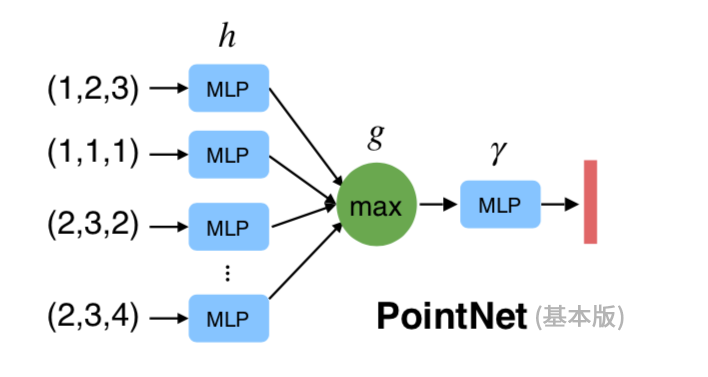
\includegraphics[width=.48\textwidth]{vanillapointnet}}%
	\hspace{0em}%
	\subcaptionbox{点云自动对齐网络\label{fig:pointnetinputalignment}}
	{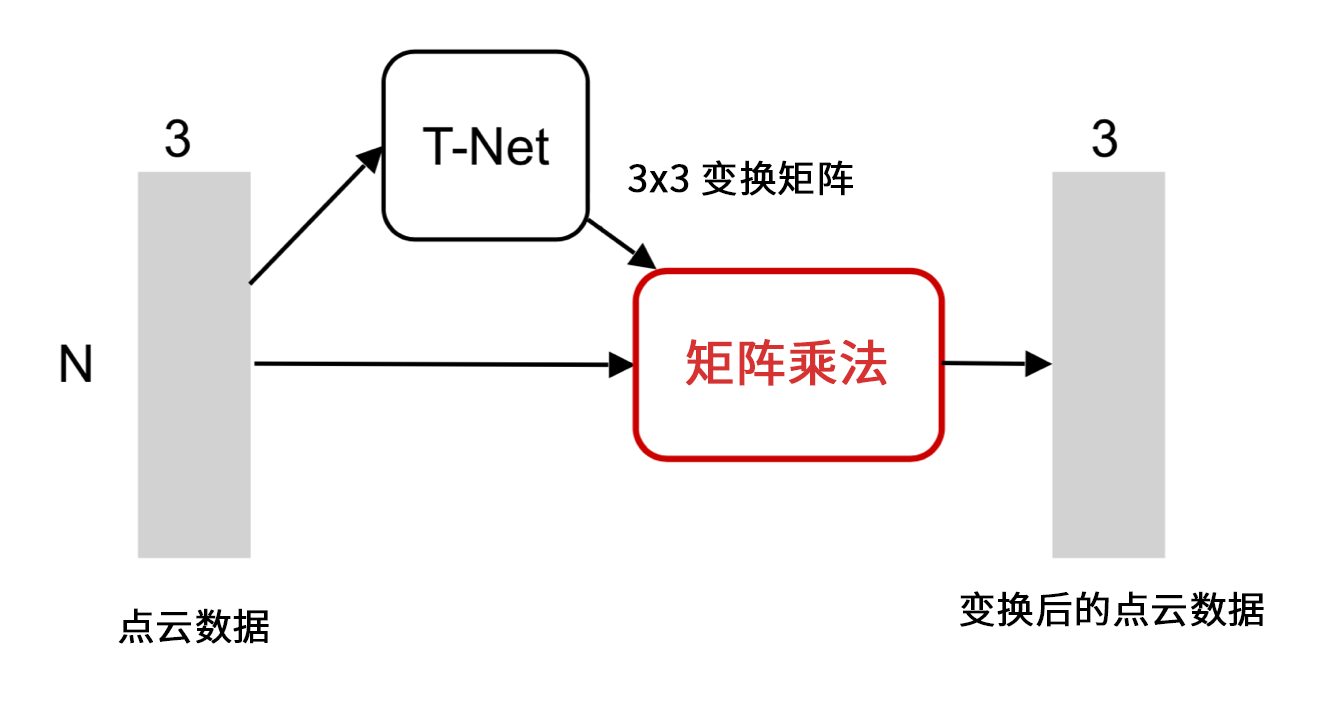
\includegraphics[width=.48\textwidth]{pointnetinputalignment}}
	\caption{PointNet\cite{pointnet} 的基本组成部件}\label{fig:pointnetelement}
\end{figure}



\subsection{点云的刚体不变性}
$\eqref{eq:symmetric}$ 只考虑了点云的排列不变性。事实上,点云数据还有刚体不变性的特点,即对任何点云数据做旋转、平移等刚体变换后,其仍然表示着同样的点云,对应的分类和分割结果不应当发生变化。

鉴于此,此工作引入了一个自动对齐点云的网络 T-Net。它可以从输入点云中自动回归出用于对齐的仿射变换矩阵。接下来只需一个矩阵乘法操作,点云的自动对齐任务就完成了,如图 \ref{fig:pointnetinputalignment} 所示。


\subsection{点云分类与分割}
通过将图 \ref{fig:pointnetelement} 中 PointNet 的基本组成部件组合,我们就得到了一个完整的点云分类与分割的网络,如图 \ref{fig:pointnetarchi}  所示。其中,对于点云分割任务来说,我们还要额外的将局部特征与全局特征相组合,确保分割结果同时兼顾到细节与整体。
\begin{figure}[h]
	\centering%
	{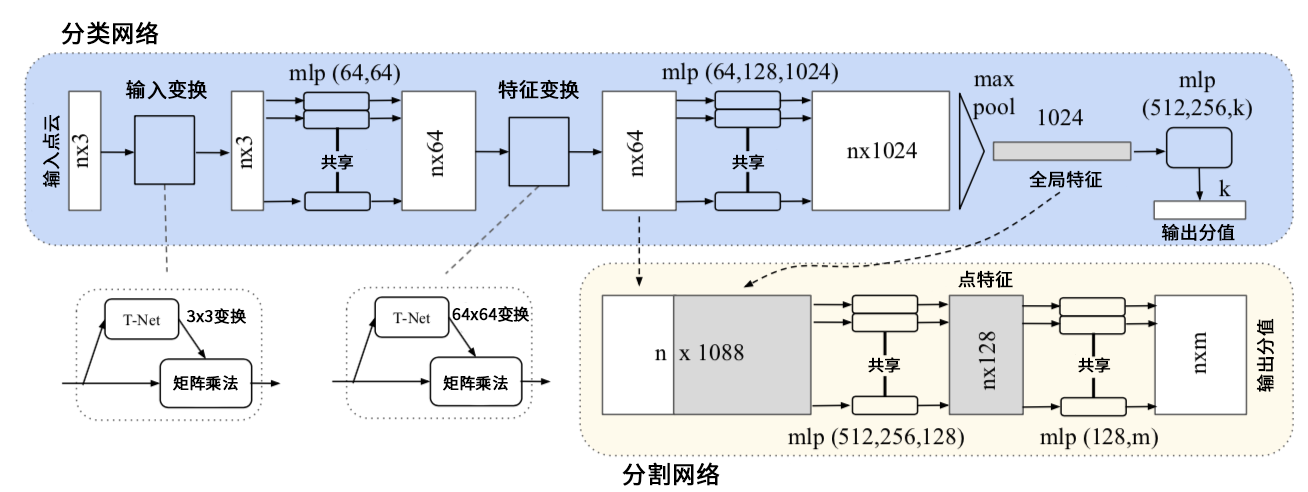
\includegraphics[width=.95\textwidth]{pointnetarchi}}
	\caption{PointNet\cite{pointnet}  的完整结构}
	\label{fig:pointnetarchi}
\end{figure}

\subsection{鲁棒性 \label{pointnet-robust}}
% \inlinecite{pointnet} 的
实验数据表明,PointNet 对点云的缺失并不敏感:即使是输入点云数据丢失了 $50\%$,其正确率也只会下降 $2\%$,如图 \ref{fig:pointnetrobust} 所示。

究其原因,我们认为是因为 $\eqref{eq:symmetric}$ 中的取最大值操作,巧妙的将模型的边、棱、角等关键点提取了出来,如图 \ref{fig:pointnetrobustvis} 第二行所示。
具体来说,对于关键点 $\bm p$ 而言,其 $h(\bm p)$ 总有一个分量值很大,因此在 $\gamma \circ \max$ 中占据了主导地位。然而,对于大部分非关键点 $\bm q$ 而言,其 $h(\bm q)$ 的各个分量值都很小,因此在 $\gamma \circ \max$ 中完全没有贡献,即它对模型的输出没有任何关联。这样的非关键点即使是缺失了,也不会对算法带来明显影响。

我们还可以进一步画出点云的上界集合,即加入后仍然不影响模型输出的点集,如图 \ref{fig:pointnetrobustvis} 第三行所示。模型对于任何介于关键点集合到上界集合的输入,都会给出同样的结果,因此 PointNet 是鲁棒的。


\begin{figure}[h]
	\centering%
	\subcaptionbox{数据丢失比例与准确率的关系\label{fig:pointnetrobust}}
	{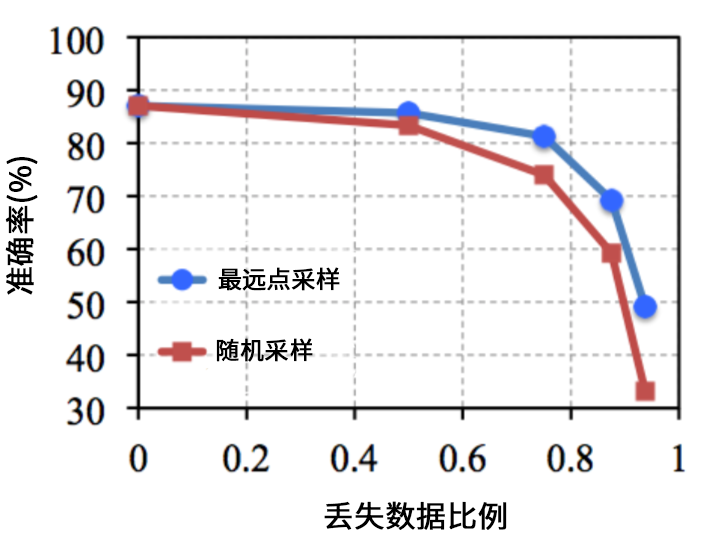
\includegraphics[width=.40\textwidth]{pointnetrobust}}%
	\hspace{2em}%
	\subcaptionbox{关键点集合与上界集合的可视化\label{fig:pointnetrobustvis}}
	{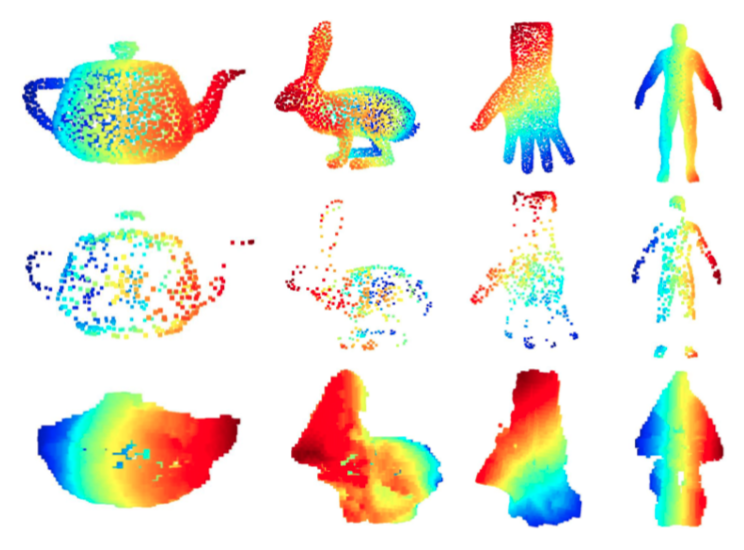
\includegraphics[width=.45\textwidth]{pointnetrobustvis}}
	\caption{PointNet\cite{pointnet}  的鲁棒性及其可视化}
\end{figure}

尽管 PointNet 鲁棒性提升了其在分类和分割问题中表现,然而在第 \ref{section:gen3d} 节中我们会看到,它 的鲁棒性会对三维点云的生成问题带来一定的麻烦。

\subsection{改进:局部细节的提取}
通过 $\eqref{eq:symmetric}$ 和图 \ref{fig:vanillapointnet},我们可以观察到:PointNet 特征提取是一种全局化方式,并不像卷积神经网络一样,重视局部细节的提取。正如我们在 \ref{section:pcintro} 节中所介绍的一样,点云的局部细节提取是很麻烦的,因此这个工作并没有对此进行过多的考虑。

事实上,目前已经有相当多的工作对于点云的局部细节提取作出了改进,如:
PointNet++\cite{pointnet2}、Kd-Net\cite{kdnet}、PointCNN\cite{pointcnn}、DGCNN\cite{dgcnn} 等。
限于篇幅,我们不再对它们逐个展开介绍。

\section{其他问题与未来展望}
除了点云生成、分类、分割以及将在第  \ref{section:gen3d} 节中详细介绍的点云生成外,目前有相当多的新工作,成功地用点云解决了更多也更具有挑战性的%点云三维深度学习
问题,
如点云场景检索\cite{pointnetvlad}、点云物体检测\cite{frustumpointnet}等。激动人心的是,现在已经有前沿工作,将点云三维深度学习中的思想和方法应用于基于三角面片的三维深度学习问题中,
如 AtlasNet\cite{atlasnet} 等。这向我们展示了点云的强大威力,同时也见证了点云对于三维深度学习发展所做出的不可磨灭的贡献。

也许有一天,点云会完成其历史使命,并悄然无息地退出三维深度学习的舞台。而取而代之的将是三角面片等更高级、更自然、更准确、更完善的三维模型表示方式。
但我们相信,没有点云相关工作的推进,就很难有三维深度学习的美好未来。

% 其他:点云检索,点云识别

\chapter{深度生成模型}
\label{cha:gen}

在机器学习中,数据的合成与采样是一类重要的研究课题。
它的基本目标是:按照训练数据的分布规律进行采样,生成一系列相似的新样本,
即使得模型的概率分布 $\PMODEL(\bm x)$ 尽可能的接近训练数据的概率分布 $\PDATA(\bm x)$:
\begin{align}
	\PMODEL(\bm x) \approx \PDATA(\bm x) \label{eq:densityestimation}
\end{align}
数据的概率分布 $\PDATA(\bm x)$ 通常不会显式地给出,而是在训练数据集中以采样的形式间接提供。
而深度生成模型,顾名思义,正是使用深度学习解决此类问题的有效手段。


\begin{figure}[h]
	\centering%
	{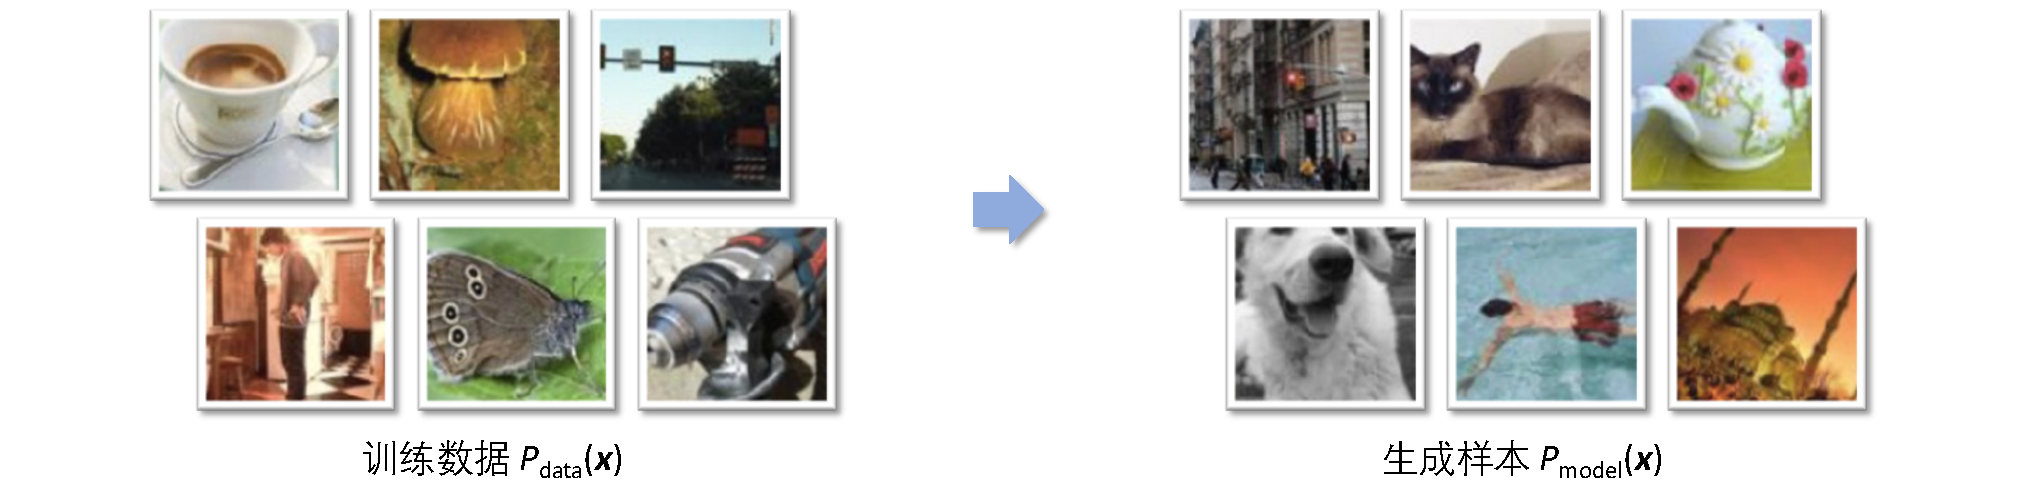
\includegraphics[width=.99\textwidth]{imggen}}
	\caption{图像生成问题\cite{gantutorial}}\label{fig:imggen}
\end{figure}

合成与采样任务通常对数据的形式没有任何假设,
因此,其外延涵盖了图像生成、视频生成、文本生成、语音生成等各类任务,而不仅仅局限于图像生成。
% 它通常一个概率模型 $\PMODEL(\bm x)$,即模型的输出并不是一成不变的,而具有一定的随机性。
但是,为了简单起见,本章仅仅以图像生成为例,讲解深度生成模型的原理与方法。
如果不加以特殊说明,在本章中深度生成模型均指代图像的深度生成模型%,而在 \ref{section:gen3d} 节中均指代点云的深度生成模型
。

\section{深度生成模型的分类}
深度生成模型所求解的 \eqref{eq:densityestimation} 实际上是无监督学习中的密度估计问题。按照是否显式地定义并优化
$\PMODEL(\bm x)$,主要的方法被分为两大类:
\begin{itemize}
	\item 显式密度估计:显式的定义模型的分布 $\PMODEL(\bm x)$,且此定义参与优化过程;
	\item 隐式密度估计:给出可按分布 $\PMODEL(\bm x)$ 采样的模型,但 $\PMODEL(\bm x)$ 没有被显式定义,也不直接参与优化过程。
\end{itemize}
\begin{figure}[h]
	\centering%
	{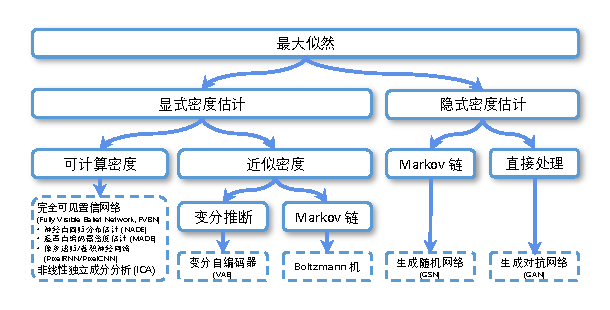
\includegraphics[width=.99\textwidth]{gentype}}
	\caption{深度生成模型的分类\cite{gantutorial}}\label{fig:gentype}
\end{figure}
按照模型所使用的密度估计方法以及具体的实现方式,深度生成模型可以被进一步细分\cite{gantutorial},如图 \ref{fig:gentype} 所示。其中,目前最常用的有以下四种:
\begin{itemize}
	\item 变分自编码器\cite{vae} (Variational Autoencoder, VAE);
	\item 生成对抗网络\cite{gan} (Generative Adversarial Network, GAN);
	\item 像素递归神经网络\cite{pixelrnn} (Pixel Recurrent Neural Networks, PixelRNN);
	\item 像素卷积神经网络\cite{pixelcnn} (Pixel Convolutional  Neural Networks, PixelCNN)。
\end{itemize}

本章将主要介绍 VAE 与 GAN。

\section{数学准备}
为了更清楚地阐述本章内容,本节补充介绍一些必要的数学概念。

\subsection{Bayes 公式}
Bayes 公式如 \eqref{eq:bayes} 所示,它表明了后验概率密度 $p(\bm z | \bm x)$、先验概率密度 $p(\bm z)$以及似然函数 $p(\bm x | \bm z)$ 三者间的关系:

\begin{align}
	%p(\bm \theta | \bm x) = \frac{p(\bm x |  \bm \theta) \cdot p(\bm \theta)}{p(\bm x)} \label{eq:bayes}
	p(\bm z | \bm x) = \frac{p(\bm x | \bm z) \cdot p(\bm z)}{p(\bm x)} \label{eq:bayes}
\end{align}
% 其中 $p(\bm \theta | \bm x)$ 为后验概率密度,$p(\bm \theta)$ 为先验概率密度,$p(\bm x | \bm \theta)$ 为似然函数。
% 其中 $p(\bm z | \bm x)$ 为后验概率密度,$p(\bm z)$ 为先验概率密度,$p(\bm x | \bm z)$ 为似然函数。
其中,我们通常把观测量 $\bm x$ 的概率密度 $p(\bm x)$ 视为常数。

% \begin{itemize}
%     \item $p(\bm \theta | x)$ 为后验概率密度;
%     \item $p(x | \bm \theta)$ 为先验概率密度;
%     \item $p(x | \bm \theta)$ 为似然函数。
% \end{itemize}

\subsection{多维正态分布}
多维正态分布又称多维 Gauss 分布,是常用概率分布之一。其参数有两个,分别是期望向量 $\bm \mu$ 和正定对称的协方差矩阵 $\bm \Sigma$。
% 若随机向量 \bm x \sim \NormDist(\bm \mu, \bm \Sigma)$,则
对于 $n$ 维的情况,其概率密度函数为
\begin{align}
	p_{\bm x \sim \NormDist(\bm \mu, \bm \Sigma)}(\bm x) =
	\sqrt{\frac{1}{(2\pi)^n |\bm\Sigma|}} \cdot
	\exp \left(- \frac{1}{2} (\bm x - \bm \mu)^T \Sigma^{-1} (\bm x - \bm \mu)\right)
	\label{eq:normdist}
\end{align}

%(一维)正态分布 $\NormDist(\mu, \sigma^2)$ 即 $\bm \mu = \mu, \bm \Sigma = \sigma^2$ 的多维正态分布。 
\subsection{Kullback-Leibler (KL) 散度与 Jensen–Shannon (JS) 散度}
要衡量两个概率分布 $p(\bm x)$ 与 $q(\bm x)$ 的差异程度,我们可以使用散度。

在统计学中,
散度 $\Div{\cdot}{\cdot}$ 是一个泛函,其输入为两个
%同支撑集的
概率密度函数 $p(\bm x)$ 与 $q(\bm x)$,输出为一个实数,且满足
\begin{itemize}
	\item $\Div{p}{q} \ge 0, \quad  \forall p, q$;
	\item $\Div{p}{q} = 0 \, \Leftrightarrow \, p(\bm x) = q(\bm x), \, \text{  a. e.}$。
\end{itemize}
可以证明:
\begin{align}
	\DKL{p}{q} & = \EXPECT{\bm x \sim p}{\left[ {\log \frac{p(\bm x)}{q(\bm x)}} \right]} \label{eq:kldiv} \\
	\DJS{p}{q} & =
	\frac{1}{2}\, \DKL*{p}{\frac{p + q}{2}} +
	\frac{1}{2}\, \DKL*{q}{\frac{p + q}{2}} \label{eq:jsdiv}
\end{align}
都满足散度定义,因此我们把 \eqref{eq:kldiv} 称为 KL 散度,把 \eqref{eq:jsdiv} 称为 JS 散度。

值得注意的是,虽然 JS 散度是对称的,但 KL 散度却不对称,即:
$\forall p, q, \DJS{p}{q} = \DJS{q}{p}$;$\exists p, q, \DKL{p}{q} \ne \DKL{q}{p}$。%因此,我们不可以将 KL 散度称为两概率分布间的“距离”。
因此,计算 KL 散度时一定不能混淆两概率分布的先后顺序。




\subsection{$K$-Lipschitz 连续 与 Lipschitz 常数}
若函数 $f: \mathbb{R}^n \to \mathbb{R}$ 满足
\begin{align}
	\Norm*{f\left( \bm x_1 \right)-f\left( \bm x_2 \right)} \leq K \cdot \Norm*{\bm x_1-\bm x_2}
	\label{eq:lip}
\end{align}
则称其是 $K$-Lipschitz 连续的。满足 \eqref{eq:lip} 的最小 $K$ 称为函数 $f$ 的 Lipschitz 常数,记为
$\Norm{f}_{\mathrm{Lip}}$。











\section{引入:自编码器 (Autoencoder, AE) \label{section:ae}}
自编码器是用于提取数据低维特征的有力武器,其架构如图 \ref{fig:ae} 所示。

\begin{figure}[h]
	\centering%
	{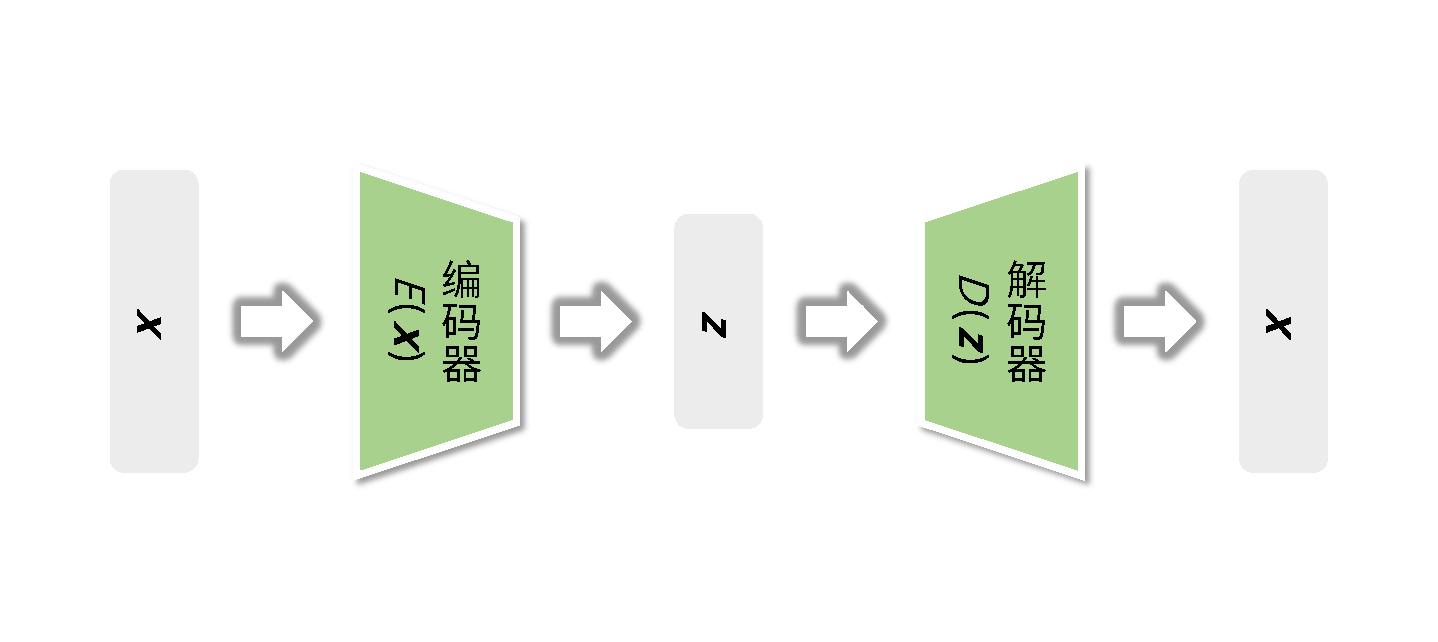
\includegraphics[width=.99\textwidth]{ae}}
	\caption{自编码器}\label{fig:ae}
\end{figure}

自编码器通常包括编码器 $E$、一个解码器 $D$ 和一个隐表示层 $\bm z$。
对于任意的数据 $\bm x$,编码器首先将其编码为隐向量 $\bm z = E(\bm x; \bm\theta_E)$。
随后,解码器对其进行重建 $\bm {\hat x} = D(\bm z; \bm\theta_D)$。
自编码器的目标是通过最小化重建误差
\begin{align}
	\Loss(\theta_E, \theta_D) = \sum_k \Norm{\bm  x_k - \bm {\hat x}_k}^2 \label{eq:aeloss}
\end{align}
来确保输入数据 $\bm x$ 能够尽可能地被编码且准确恢复。其中 $k$ 表示训练数据的编号。

通常来说,$\bm z$ 的维度要远远低于 $\bm x$,因为
这样的设计会强制自编码器捕获到数据最显著的差异,亦即特征,而忽略掉无意义的信息。
否则,如果 $\bm z$ 的维度与 $\bm x$ 的维数持平或者更高,则自编码器不会主动的完成特征提取的任务。

自编码器是一种无监督的方法,即不必提供成对的标注数据,即可完成低维特征的提取。
虽然它不是一个深度生成模型,但它启发了深度生成模型 VAE 的设计。
我们将在第 \ref{section:vae} 节简要介绍它。

















\section{变分自编码器 (Variational Autoencoder, VAE) \label{section:vae}}
与自编码器类似,VAE\cite{vae} 的基本想法是:假设数据 $\bm x $ 是根据一个不可见的隐向量 $\bm z \sim \NormDist(\bm 0, \bm I)$,按照概率 $p(\bm x | \bm z; \bm \theta)$ 生成出来的:
\begin{align}
	\PMODEL(\bm x; \bm\theta) = \int_{\bm z} p(\bm x | \bm z; \bm\theta) \cdot p(\bm z) \cdot d\bm{z} \label{eq:vaepmodel}
\end{align}
% 与自编码器类似,\eqref{eq:vaepmodel} 中的似然函数 $p(\bm x | \bm z; \bm\theta)$ 也被称为解码器网络。
其中的似然函数 $p(\bm x | \bm z; \bm\theta)$ 也被称为解码器网络,与自编码器的命名方式类似。


根据最大似然估计,为了%尽量
尽可能满足 \eqref{eq:densityestimation},我们需要求出网络参数 $\bm\theta$ 来最大化 $\log \PMODEL(\bm x; \bm\theta)$。
但稍加分析,我们就会发现,数据似然函数 $\PMODEL(\bm x; \bm\theta)$ 与后验分布 $p(\bm z | \bm x; \bm\theta)$ 均不能有效计算,因此我们要另辟蹊径。

文献 \inlinecite{vae} 提出了一个创造性的想法:用一个新的编码器网络 $q(\bm z | \bm x; \bm\phi)$ 来近似不能有效计算的后验分布 $p(\bm z | \bm x; \bm\theta)$。
% 这使得我们可以推导出一个变分下界,让问题变得可解。
稍加分析,我们就会发现:
\begin{align}
	\,       & \log \PMODEL(\bm x; \bm \theta)               &                                                           & \notag \\
	= \,     & \EXPECT{\bm z \sim q(\bm z | \bm x; \bm\phi)}
	{\left[\log \PMODEL(\bm x; \bm\theta)\right]}
	         &                                               & \text{$\PMODEL(\bm x; \bm\theta)$ 与 $\bm z$ 无关} \notag          \\
	= \,     & \EXPECT{\bm z \sim q(\bm z | \bm x; \bm\phi)}
	{\left[
			\log\frac{p(\bm x | \bm z; \bm\theta) \cdot p(\bm z)}{p(\bm z | \bm x; \bm\theta)}
	\right]} &                                               & \text{Bayes 公式 \eqref{eq:bayes}}\notag                           \\
	= \,     &
	\EXPECT{\bm z} {\left[
			\log\frac{q(\bm z | \bm x; \bm\phi)}{p(\bm z | \bm x; \bm\theta)}
			\right]}
	+
	\EXPECT{\bm z} {\left[\log p(\bm x | \bm z; \bm\theta)\right]}
	-
	\EXPECT{\bm z} {\left[\log
			\frac{q(\bm z | \bm x; \bm\phi)}{p(\bm z)}
	\right]} &                                               & \text{对数运算;期望可加}\notag                                    \\
	= \,     &
	\underbrace{\DKL{q(\bm z | \bm x; \bm\phi)}{p(\bm z | \bm x; \bm\theta)}}_{\ge 0}
	\notag                                                                                                                        \\
	\,       &
	\quad \quad
	+ \underbrace{
		\EXPECT{\bm z} {\left[\log p(\bm x | \bm z; \bm\theta)\right]}
		- \DKL{q(\bm z | \bm x; \bm\phi)}{p(\bm z)}}_{\Loss(\bm \phi, \bm\theta)}
	         &                                               & \text{KL 散度的定义\eqref{eq:kldiv}}\notag                         \\
	\ge      & \,\Loss(\bm \phi, \bm \theta) \notag
\end{align}
即 $\Loss(\bm \phi, \bm \theta)$ 一定不会超过对数似然函数 $\log \PMODEL(\bm x; \bm\theta)$ 的值:
\begin{align}
	\Loss(\bm \phi, \bm\theta) =
	\underbrace{\EXPECT{\bm z} {\left[\log p(\bm x | \bm z; \bm\theta)\right]}}
	_{\text{重建损失函数}}
	-
	\underbrace{\DKL{q(\bm z | \bm x; \bm\phi)}{p(\bm z)}}
	_{\text{KL 损失函数}}
	\le \log\PMODEL(\bm x; \bm\theta)
	\label{eq:ELBO}
\end{align}
因此,我们将 $\Loss(\bm \phi, \bm \theta)$ 称为变分下界 (Variational Lower Bound, Evidence Lower Bound, ELBO)。

要最大化对数似然 $\log \PMODEL(\bm x; \bm\theta)$,我们可以通过最大化变分下界 $\Loss(\bm \phi, \bm \theta)$ 来间接地实现。那么,$\Loss(\bm \phi, \bm \theta)$ 是否可以被有效计算呢?答案是肯定的。

变分下界 $\Loss(\bm \phi, \bm \theta)$ 中的第一项 $\EXPECT{\bm z} {\left[\log p(\bm x | \bm z; \bm\theta)\right]}$ 通常被称为重建损失函数,它可以通过对 $\bm z \sim q(\bm z | \bm x; \bm\phi)$ 采样,然后计算解码器网络输出 $p(\bm x | \bm z; \bm\theta)$ 的方式求出。如果我们进一步假设解码器网络 $p(\bm x | \bm z; \bm\theta) = \NormDist\left(\bm \mu_\theta(\bm z; \bm \theta), \sigma^2 I\right)$ %为各向同性且方差固定的多维高斯分布
,那么根据 \eqref{eq:normdist},重建误差即
\begin{align}
	{%\EXPECT{\bm z}
		{%\left[
				\log p(\bm x | \bm z; \bm\theta)%\right]
			}}
	 & =
	\underbrace{\left[ - \frac{n}{2} \cdot \log\left(2\pi\sigma^2\right) \right]}_{C}
	-
	\underbrace{\left[ \frac{1}{2\sigma^2} \right]}_{\lambda} \cdot \Norm*{\bm x - \bm \mu_\theta(\bm z; \bm \theta)}^2 \notag \\
	 & = - \lambda \cdot\Norm*{\bm x - \bm \mu_\theta(\bm z; \bm \theta)}^2 + C
	\label{eq:vaerecons}
\end{align}
其中超参数 $\lambda = 1/\left(2\sigma^2\right)> 0$。这与自编码器的损失函数 \eqref{eq:aeloss} 如出一辙。

变分下界 $\Loss(\bm \phi, \bm \theta)$ 中的第二项 $\DKL{q(\bm z | \bm x; \bm\phi)}{p(\bm z)}$ 通常被称为 KL 损失函数,因为它希望近似的后验分布 $q(\bm z | \bm x; \bm\phi)$ 尽可能接近先验分布 $p(\bm z)$。
如果我们进一步假设近似的后验分布
$q(\bm z | \bm x; \bm\phi) = \NormDist
	\left(
	\bm\mu_{\bm\phi}   (\bm x; \bm\phi),
	\bm\Sigma_{\bm\phi}(\bm x; \bm\phi)
	\right)$,则 KL 损失函数项有闭合解,可被解析地算出。

综上所述,在训练 VAE 时,我们需要最大化其变分下界,即优化以下损失函数:
\begin{align}
	\argmin{\bm\theta, \bm\phi}
	- \Loss(\bm \phi, \bm \theta) & =
	\argmin{\bm\theta, \bm\phi}
	- {\EXPECT{\bm z} {\left[\log p(\bm x | \bm z; \bm\theta)\right]}}
	+ \DKL{q(\bm z | \bm x; \bm\phi)}{p(\bm z)}
	\notag                                                                      \\
	                              & = \argmin{\bm\theta, \bm\phi} \lambda \cdot %\cdot
	{\EXPECT{\bm z}{\left[\Norm*{\bm x - \bm \mu_\theta(\bm z; \bm \theta)}^2\right]}}
	+ \DKL{q(\bm z | \bm x; \bm\phi)}{p(\bm z)}
\end{align}
其中超参数 $\lambda > 0$;而要通过 VAE 生成新样本时,我们按照 \eqref{eq:vaepmodel} 采样就可以了。

VAE 在图像生成任务上的表现如图 \ref{fig:vaeimg} 所示。它的缺点是,生成的图片普遍比较模糊。
\begin{figure}[h]
	\centering%
	{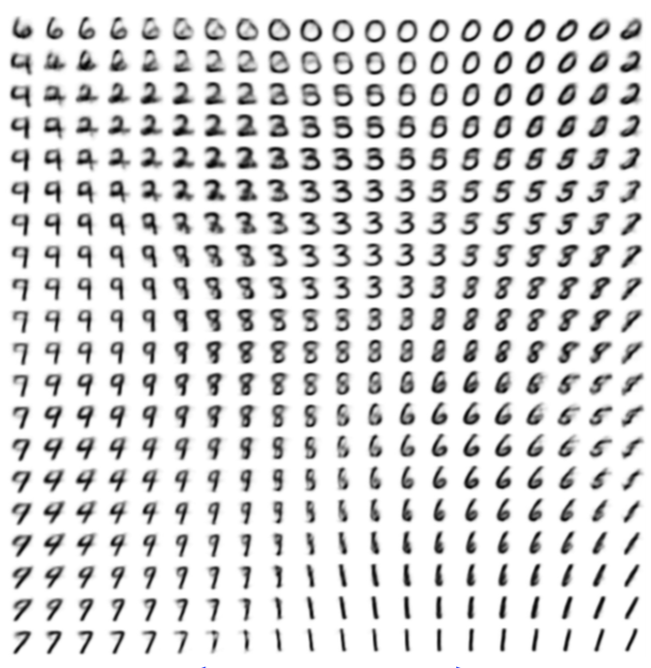
\includegraphics[width=.65\textwidth]{vaeimg}}
	\caption{使用 VAE 解决图像生成任务\cite{vae}}\label{fig:vaeimg}
\end{figure}





% GAN的改进

% WGAN, WGAN-GP
% DRAGAN
% SNGAN

\section{生成对抗网络 (Generative Adversarial Network, GAN) \label{section:gan}}
GAN\cite{gan} 是目前所有的深度生成模型中表现最出色的。图 \ref{fig:gan} 展现了其基本思想和架构。


\begin{figure}[h]
	\centering%
	{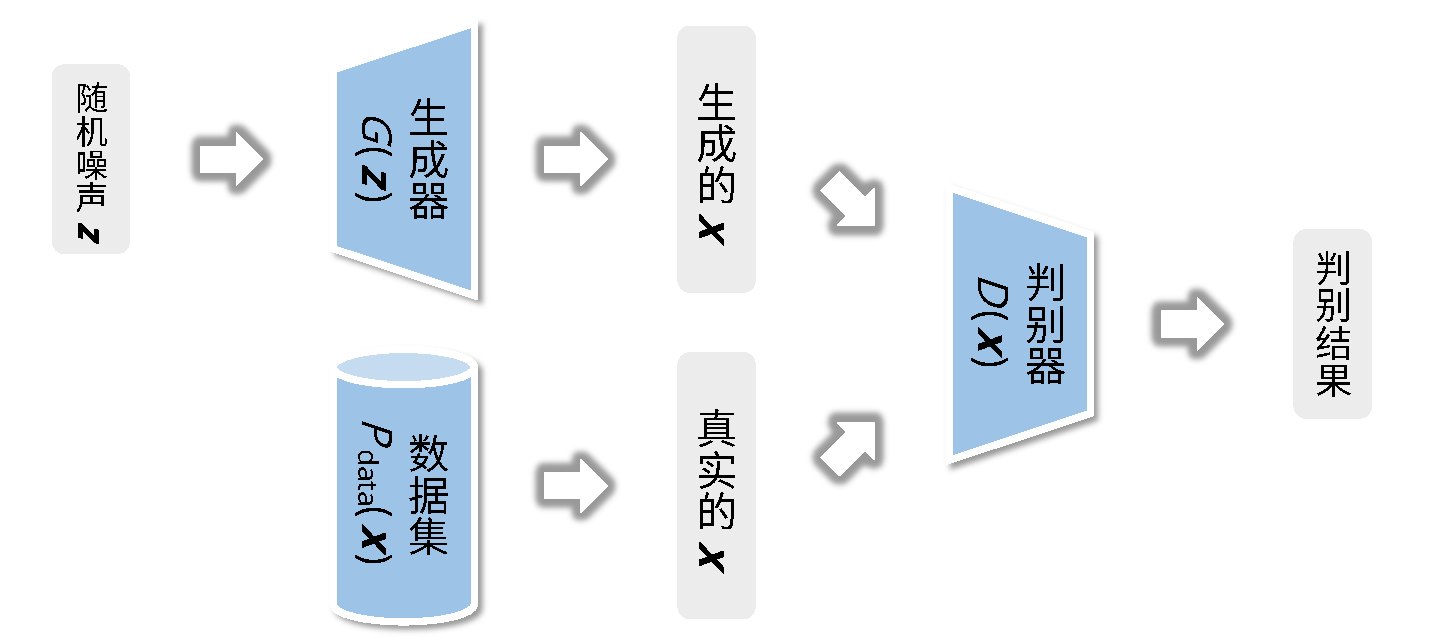
\includegraphics[width=.9\textwidth]{gan}}
	\caption{生成对抗网络}\label{fig:gan}
\end{figure}
%它的基本思想源于
GAN 创造性地将博弈论的概念引入到了深度生成模型中,建立了一个生成器网络 (Generator, $G$) 和 判别器网络 (Discriminator, $D$) 之间的博弈场景:
生成器网络 $G$ 根据隐随机向量 $\bm z \sim \NormDist(\bm 0, \bm I)$ 的观测值直接生成新样本 $\bm x = G(\bm z; \bm\theta_G)$;而判别器网络 $D$ 需要分辩出一个特定的样本是 $G$ 生成的还是训练数据集中已有的。通常,$D$ 通过输出一个概率值 $D(\bm x; \bm\theta_D) \in [0, 1]$ 的形式,来表示它的判定结果。

在这个博弈游戏中,判别器网络 $D$ 的终极目标是
%尽可能的
把 $G$ 生成的样本和数据集中已有的样本区分开,
而生成器网络 $G$ 的终极目标是生成足够接近于训练数据集的新样本,使之无法区分,以欺骗 $D$。
因此,我们可以使用一个零和博弈的过程来训练 $D$ 和 $G$。令 $D$ 的损失为 $\Loss(\bm\theta_G, \bm\theta_D)$:%其中
\begin{align}
	\Loss(\bm\theta_G, \bm\theta_D) =
	- \EXPECT{\bm x \sim \PDATA(\bm x)}           \log(    D(\bm x; \bm\theta_D))
	- \EXPECT{\bm z \sim \NormDist(\bm 0, \bm I)} \log(1 - D( G(\bm z; \bm\theta_G); \bm\theta_D))
	\label{eq:ganloss}
\end{align}
则 $G$ 的损失恰好为其相反数 $- \Loss(\bm\theta_G, \bm\theta_D)$。

在此博弈过程中,$G$ 和 $D$ 都会根据对方的决策来调整自己的决策——网络参数 $\bm \theta_G, \bm \theta_D$,以最小化自己的损失。
文献 \inlinecite{gan} 的分析表明,% 如果游戏的 Nash 均衡点 $\bm\theta_G^*, \bm\theta_D^*$ 存在,
如果 $G, D$ 有无限的表达能力,且 $D$ 可以达到最优状态 $D(\bm x; \bm\theta_D^*) = \PDATA(\bm x)/(\PDATA(\bm x) + \PMODEL(\bm x))$,那么随着训练过程的推进,$G$ 和 $D$ 将收敛于游戏的 Nash 均衡点 $\bm\theta_G^*, \bm\theta_D^*$:
\begin{subequations}
	\begin{align}
		\bm\theta_D^* = & \argmin{\bm\theta_D} \Loss(\bm\theta_G^*, \bm\theta_D)\label{eq:nash1} \\
		\bm\theta_G^* = & \argmax{\bm\theta_G} \Loss(\bm\theta_G, \bm\theta_D^*)\label{eq:nash2}
	\end{align}
\end{subequations}
这时,$G$ 生成的样本变得非常真实,完全不可区分,而 $D$ 也无法对任何输入样本进行判断,处处输出 $D(\bm x; \bm\theta_D) = \frac{1}{2}$。此时,我们就可以丢弃 $D$,直接使用 $G$ 来生成新样本。

为了模拟出上述博弈过程,我们通常先假设对方已经给出最优解,即 $\bm\theta_G = \bm\theta_G^*, \bm\theta_D = \bm\theta_D^*$,然后通过随机梯度下降 (Stochastic gradient descent, SGD) 等优化方法,交替优化式 \eqref{eq:nash1},\eqref{eq:nash2},完成 GAN 的训练。

文献 \inlinecite{gan} 指出:在实际的应用%过程
中,我们通常会使用最小化
$- \log(D( G(\bm z))$
的方式来替代 \eqref{eq:nash2} 中的最大化
$- \log(1 - D( G(\bm z))$ 的过程,因为前者能够再训练初期为 $G$ 提供更强的梯度信息,从而加速收敛过程。

综上所述,要训练 GAN,我们在实践中%实践中会%使用 SGD 等优化方法,
通常会交替最小化以下损失函数:
\begin{subequations}
	\label{eq:ganloss0}
	\begin{align}
		\Loss_D(\bm\theta_D; \bm\theta_G) & =
		- \EXPECT{\bm x \sim \PDATA(\bm x)}           \log(    D(\bm x; \bm\theta_D))
		- \EXPECT{\bm z \sim \NormDist(\bm 0, \bm I)} \log(1 - D( G(\bm z; \bm\theta_G); \bm\theta_D))
		\label{eq:ganloss1}                   \\
		\Loss_G(\bm\theta_G; \bm\theta_D) & =
		- \EXPECT{\bm z \sim \NormDist(\bm 0, \bm I)} \log(D( G(\bm z; \bm\theta_G); \bm\theta_D))
		\label{eq:ganloss2}
	\end{align}
\end{subequations}

GAN 在图像生成任务上的表现非常出色,如图 \ref{fig:ganimg} 所示。除了能生成图像外,GAN 还可以对图像进行插值。如图 \ref{fig:ganinter} 所示。
\begin{figure}[h]
	\centering%
	\subcaptionbox{图像生成\label{fig:ganimg}}
	{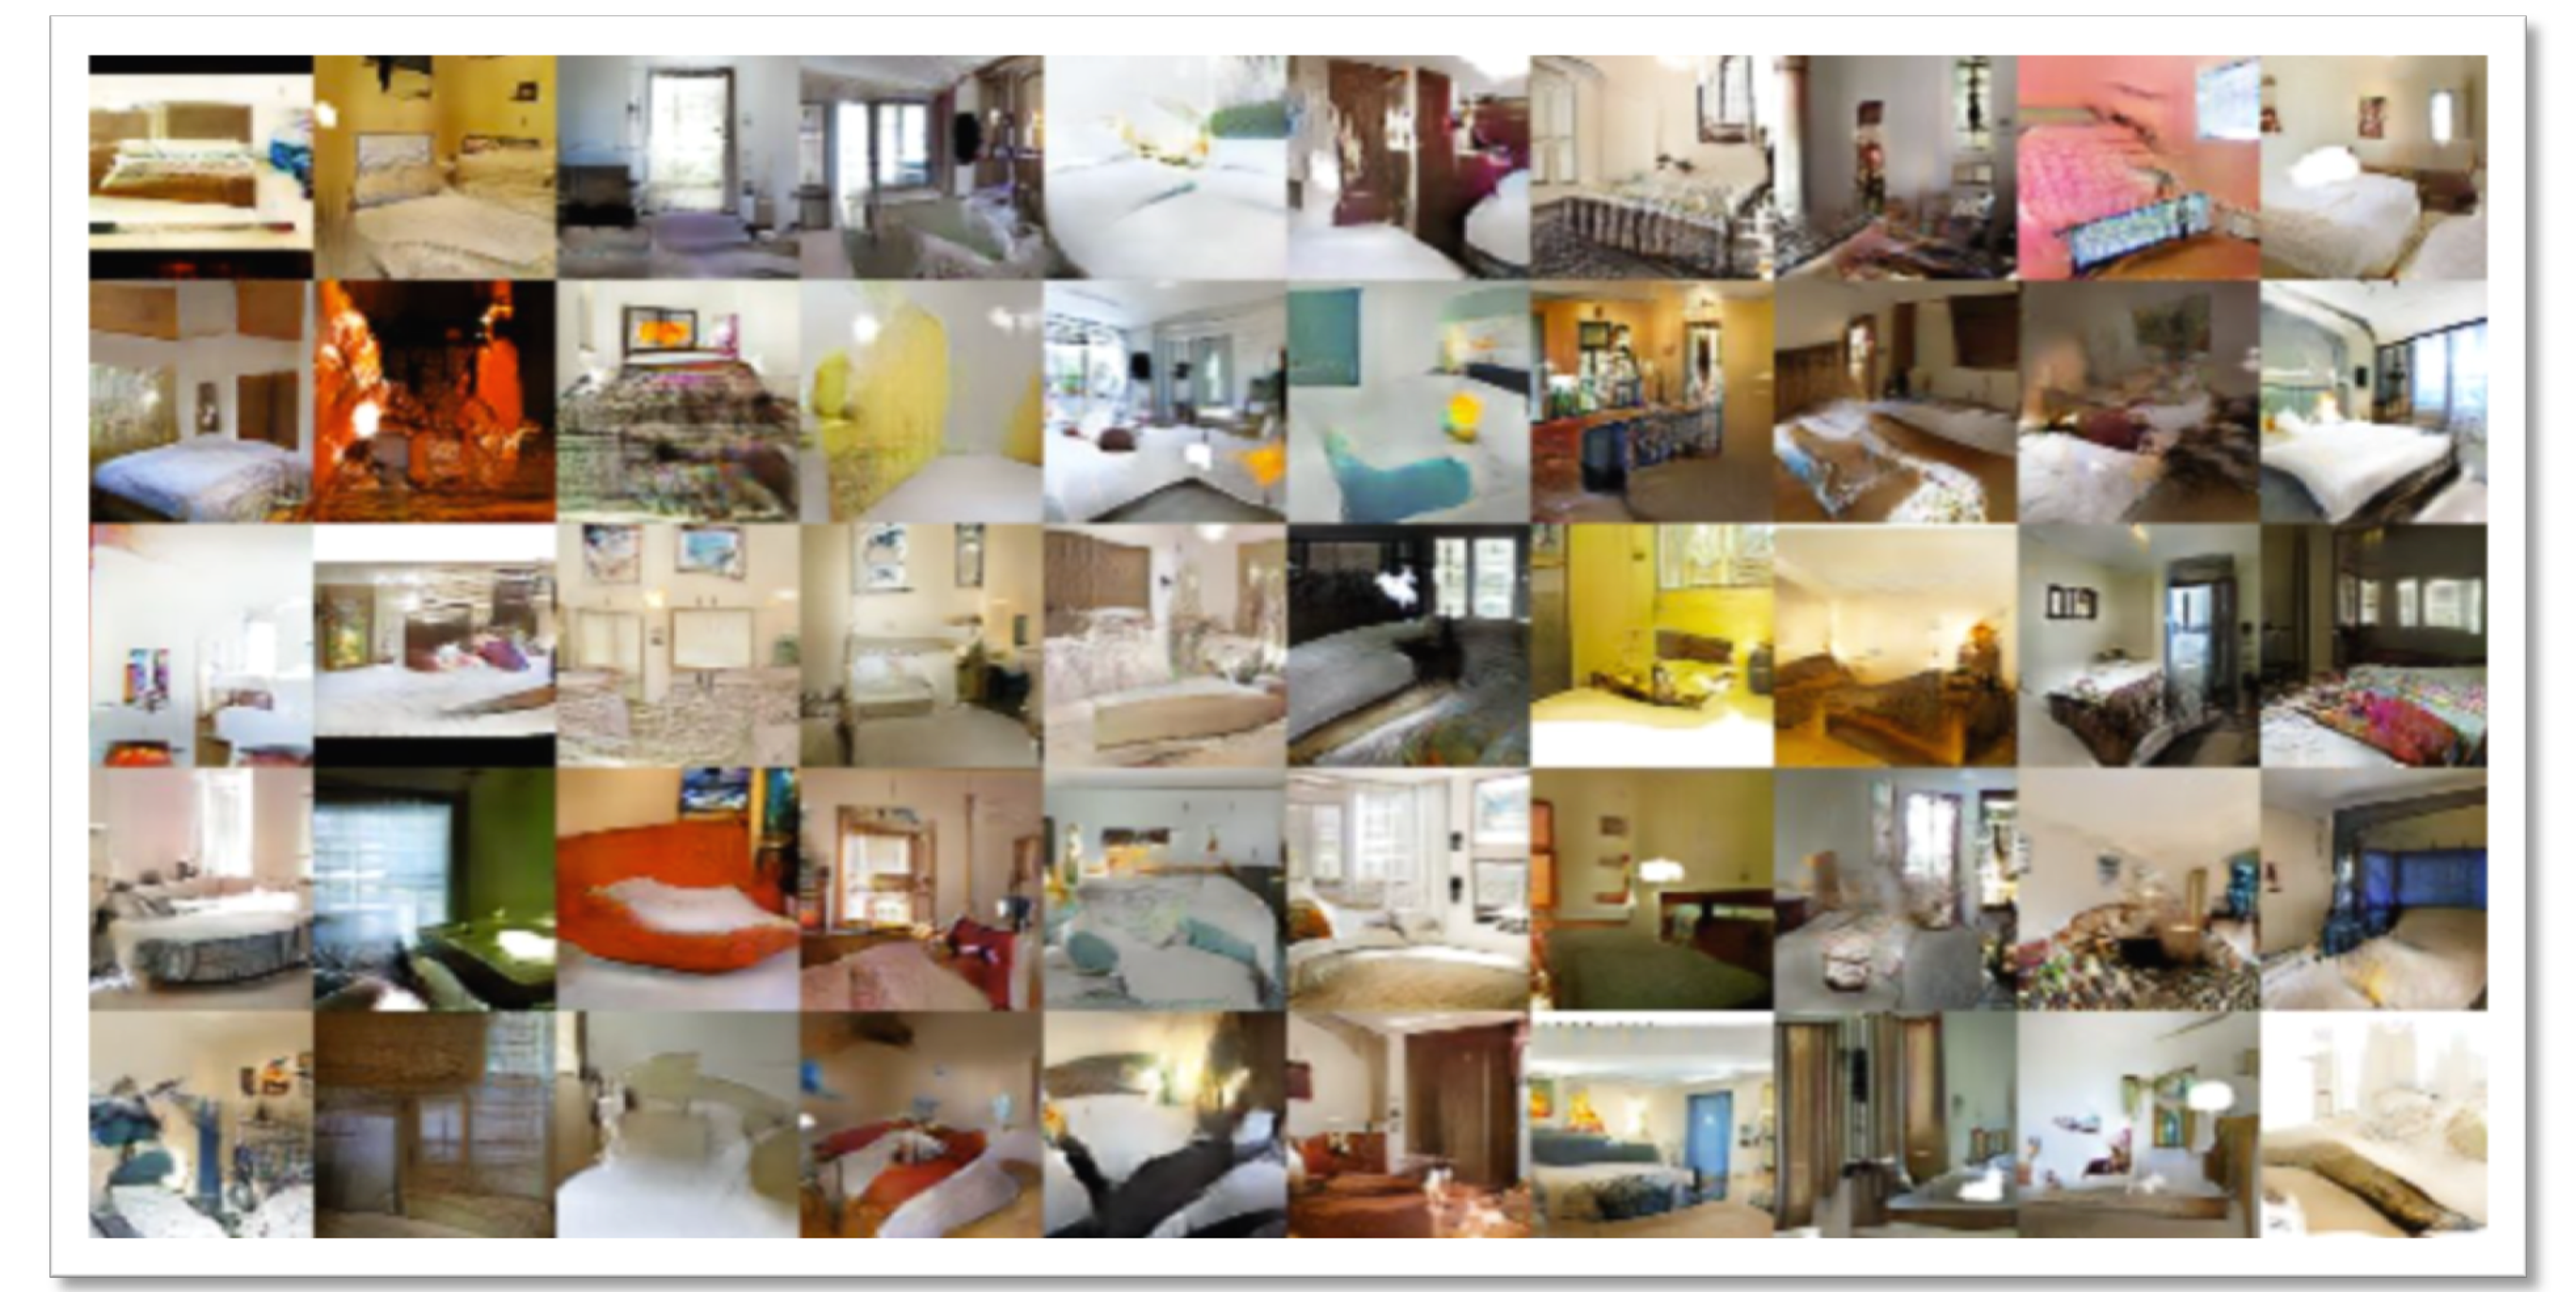
\includegraphics[width=.45\textwidth]{ganimg}}%
	\hspace{2em}%
	\subcaptionbox{图像插值\label{fig:ganinter}}
	{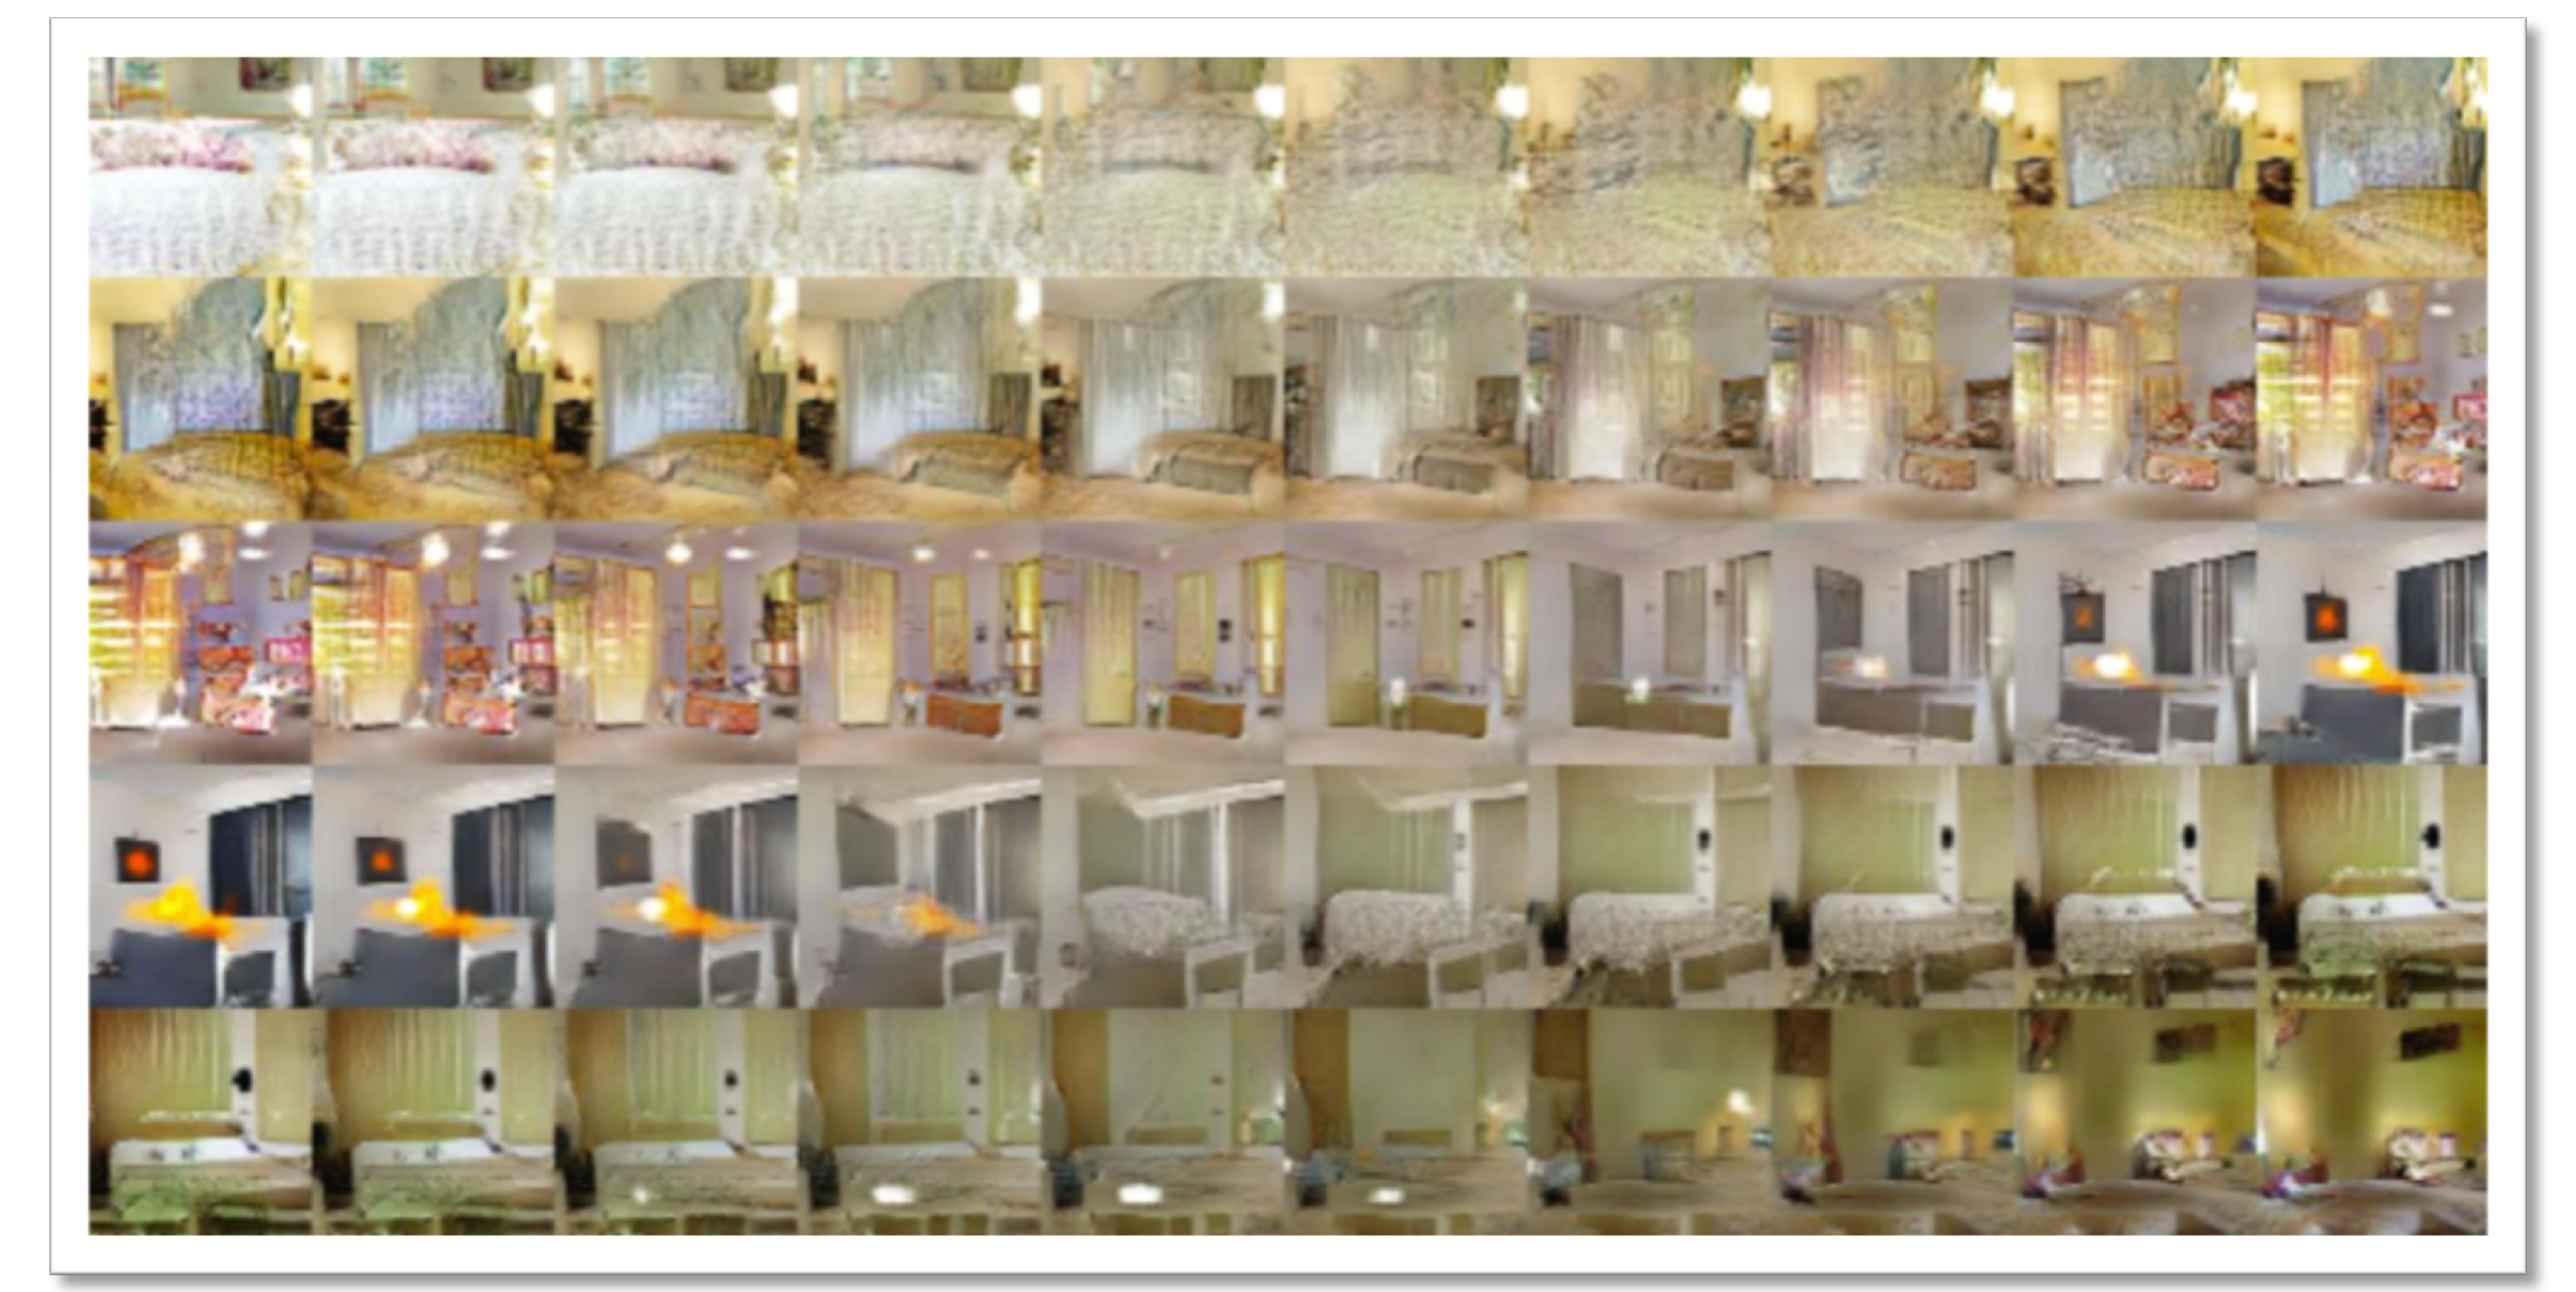
\includegraphics[width=.45\textwidth]{ganinter}}
	\caption{使用 GAN 解决图像生成任务\cite{dcgan}}
\end{figure}

尽管如此,GAN 却有训练困难、不稳定的问题。
此外,
在一些极端情况下,$G$ 还有可能会陷入只能生成一个样本或多个样本的状态,如图 \ref{fig:ganmodecollapse} 所示。
这种现象被称为模式坍塌。
我们将在第 \ref{section:ganimprove}、\ref{section:vaegan} 节中%详细
分别讨论现有研究是如何提升 GAN 的稳定性并解决模式坍塌问题的。

\begin{figure}[h]
	\centering%
	{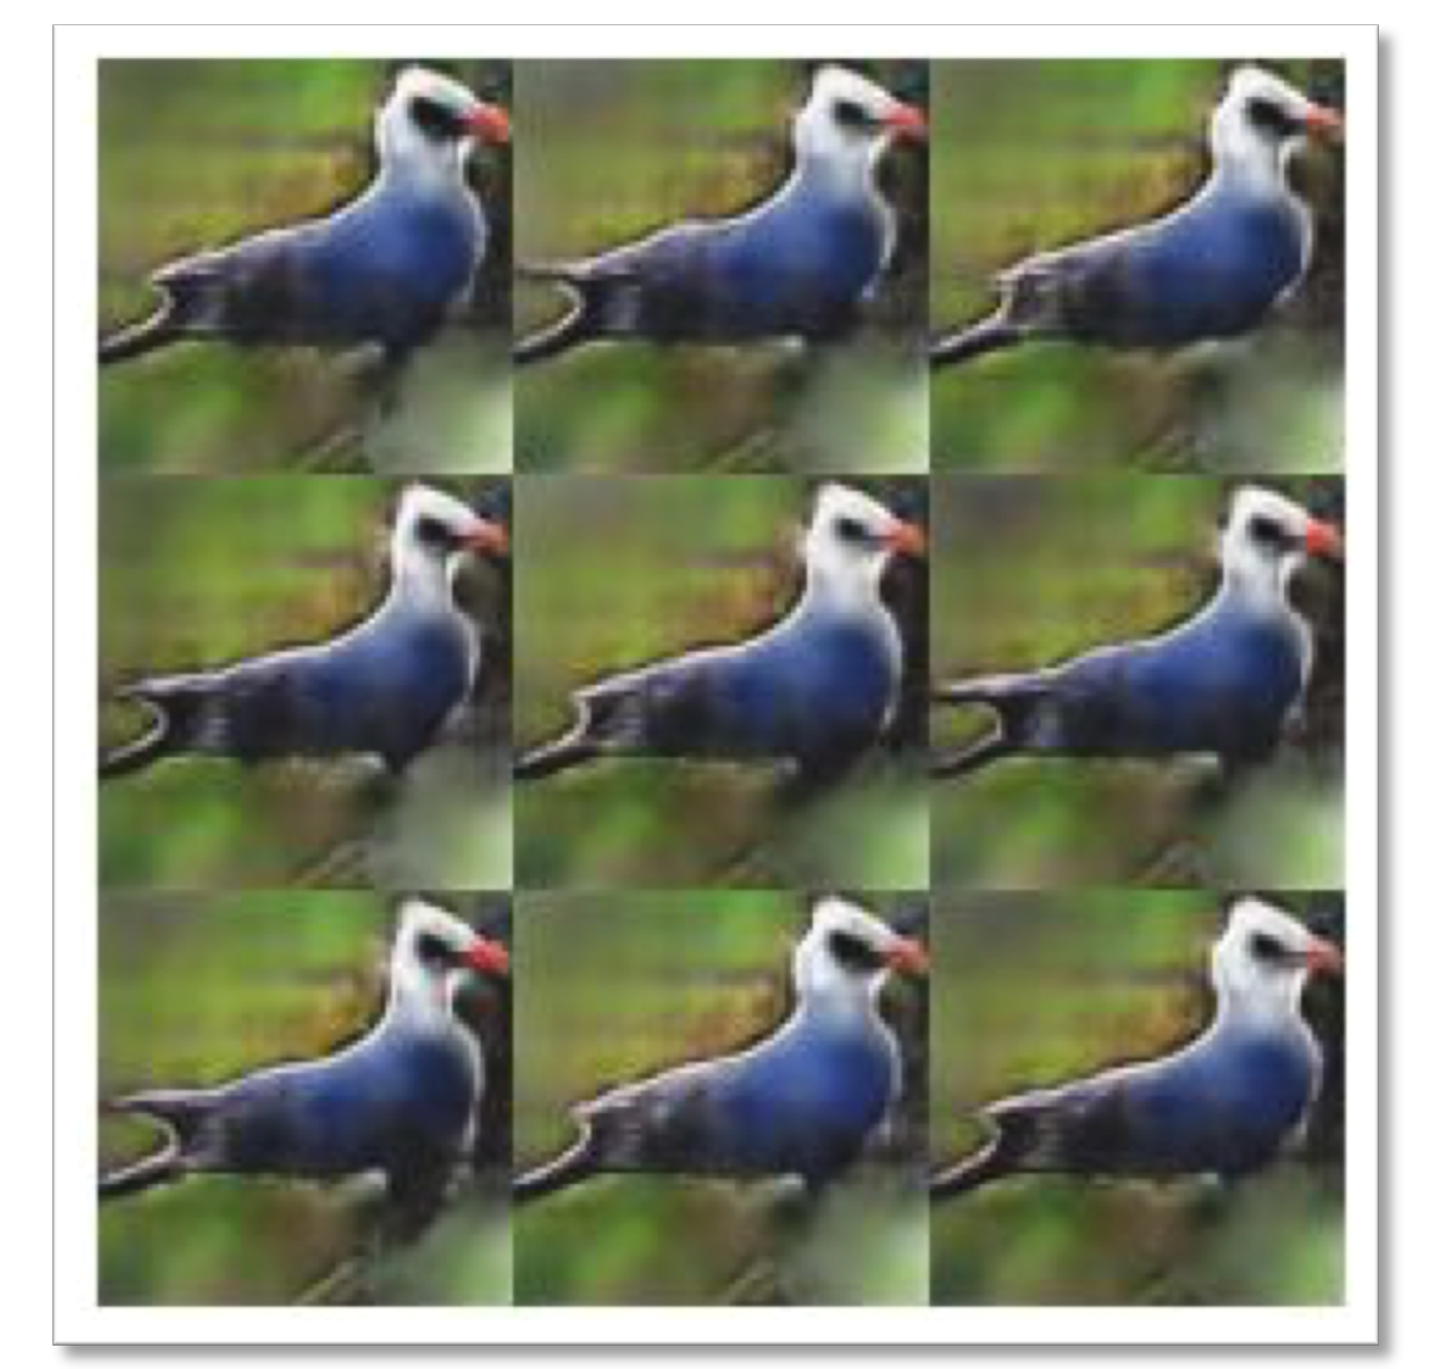
\includegraphics[width=.3\textwidth]{ganmodecollapse}}%
	\caption{GAN 的模式坍塌问题}\label{fig:ganmodecollapse}
\end{figure}
%,因为 GAN 的稳定性对 $D, G$ 的架构设计和超参数的选择非常敏感。

\section{改进 GAN 的稳定性:梯度惩罚和正则化方法 \label{section:ganimprove}}
GAN 的稳定性对 $D, G$ 的架构和超参数非常敏感,只有精心设计与选择它们,才可以得到较好的结果\cite{dcgan}。那么,导致 GAN 不稳定的原因是什么呢?

文献 \inlinecite{wganbefore} 指出:当判别器网络 $D$
达到最优状态 $D(\bm x; \bm\theta_D^*) = \PDATA(\bm x)/(\PDATA(\bm x) + \PMODEL(\bm x))$时,
式 \eqref{eq:ganloss} 可进一步简化为
\begin{align}
	\Loss(\bm\theta_G, \bm\theta_D^*) = 2\log 2 - 2 \DJS{\PDATA}{\PMODEL} \label{eq:ganlossjs}
\end{align}
此时,如果 $\PDATA(\bm x)$ 和 $\PMODEL(\bm x)$ 的支撑集之交为零测度集,那么可以证明 $\DJS{\PDATA}{\PMODEL} \equiv \log 2$,即
\begin{align}
	\Loss(\bm\theta_G, \bm\theta_D^*) \equiv 0 \label{eq:nograd}
\end{align}
这意味着生成器网络 $G$ 不能从损失函数中获取有效的梯度信息,即 $G$ 不知道如何调整决策 $\bm\theta_G$ 来降低自己的损失,训练过程就此终止。这种现象被称为梯度消失或者梯度弥散。

% 近年来,GAN的稳定训练一直是研究人员尝试攻克的重点问题。
实际上,由于 $\bm z$ 的维数通常远远低于 $G(\bm z)$ 的维数,而数据 $\bm x$ 如图像等均有信息冗余,故
$\PDATA(\bm x), \PMODEL(\bm x)$ 的支撑集都是高维空间中低维流形。在初始化阶段,其交集为零测度集的概率是 $100\%$!
因此,文献 \inlinecite{wganbefore} 中假设是绝非毫无根据、信口开河。%信口雌黄、危言耸听。%,其发生的概率是 $100\%$。

综上所述,在 $D$ 学习得
%的表现
相对较好的时候,$G$ 很有可能不知道如何调整 $\bm\theta_G$,以改善自己的表现。
要稳定训练 GAN,我们不得不平衡好 $D, G$ 的训练程度。这是导致 GAN 训练困难、
不稳定的根本原因。

为了改善 GAN 的稳定性,一种可行的方案是更改 \eqref{eq:ganloss},使得等价的优化目标不再是 $\PDATA$ 和 $\PMODEL$ 之间的散度,而是某种积分概率度量 (Integral Probability Metric, IPM),如 Wasserstein 距离\cite{wgan, wgangp} 等。这使得 $\Loss(\bm\theta_G, \bm\theta_D^*)$ 不再为恒定常数,其梯度信息可以被 $G$ 有效获取。

%,即使 $\bm\theta_G, \bm\theta_D$ 的支撑集之交为零测度集。

一些近期的研究\cite{ganestimation, lsgan2}则建议采用另一种方案:限制 $D(\bm x; \bm\theta_D)$ 必须满足 $K$-Lipschitz 连续条件。容易发现,一旦对 $D$ 施加上述限制,由 Lipschitz 连续的定义 \eqref{eq:lip},$D$ 就不再具备达到最优状态 $D(\bm x; \bm\theta_D^*)$ 的条件,式 \eqref{eq:ganlossjs}及其推论均不再成立。
\inlinecite{lsgan2} 进一步证明了,Lipschitz 连续条件能够使得训练过程有效收敛。
而按照限制 $D$ 的具体实现方案,这些工作可以被进一步分类为梯度惩罚\cite{wgangp, lsgan2, dragan}和正则化方法\cite{wgan, orthogan, sngan} 两类。




% VAE-GAN

\section{避免 GAN 的模式坍塌:VAE/GAN \label{section:vaegan}}
在第 \ref{section:gan} 节中,我们介绍了 GAN 的模式坍塌问题。但反观 VAE,我们从未发现类似的问题。
事实上,VAE 的重建误差项 \eqref{eq:vaerecons} 确保了 VAE 不会发生模式坍塌。

既然 GAN 能够生成以假乱真的高质量样本,而 VAE 又有效避免模式坍塌,那么我们可否可以取长补短,将这两者结合起来呢?
文献 \inlinecite{vaegan, cvaegan} 的工作正是这样的尝试。

我们将第 \ref{section:vae} 节介绍的 VAE 和
第 \ref{section:gan} 节介绍的 GAN 结合起来,同时合并 VAE 的解码器网络 $E$ 的 GAN 的生成器网络 $G$,
就得到了 VAE/GAN,如图\ref{fig:vaegan} 所示。
\begin{figure}[h]
	\centering%
	\subcaptionbox{网络架构\label{fig:vaegan}}
	{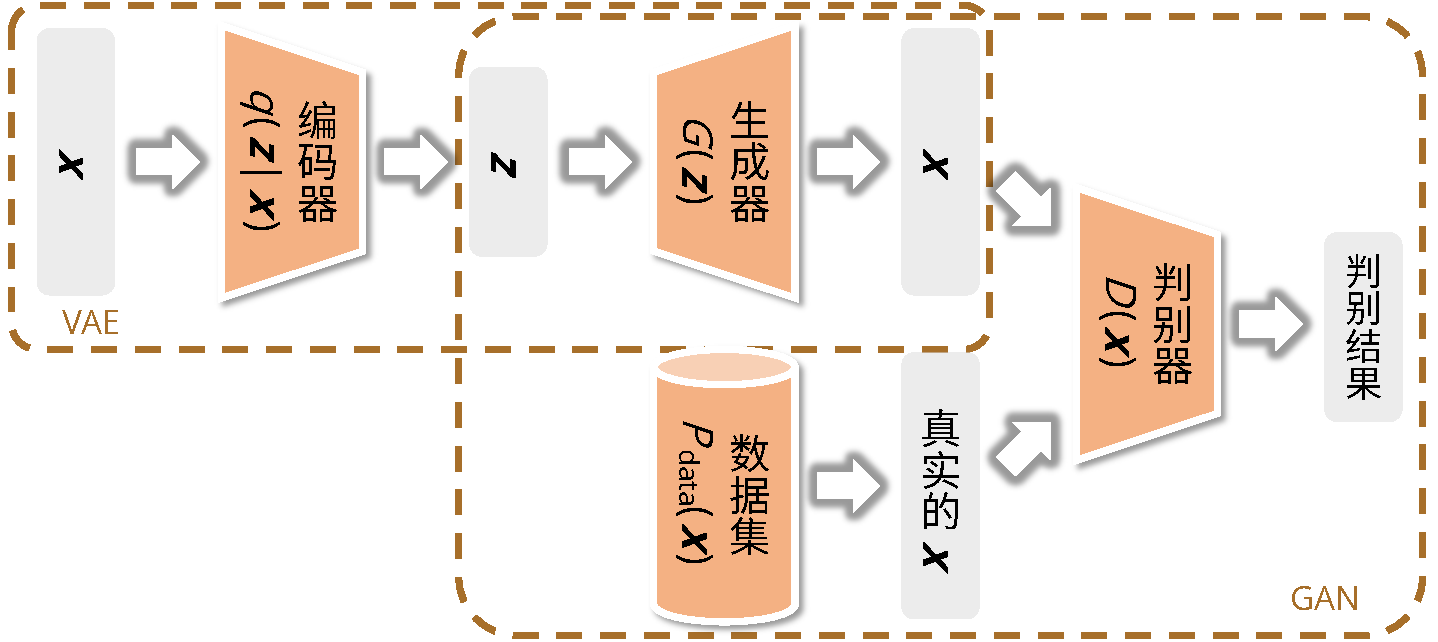
\includegraphics[width=.45\textwidth]{vaegan}}%
	\hspace{2em}%
	\subcaptionbox{损失函数\label{fig:vaeganloss}}
	{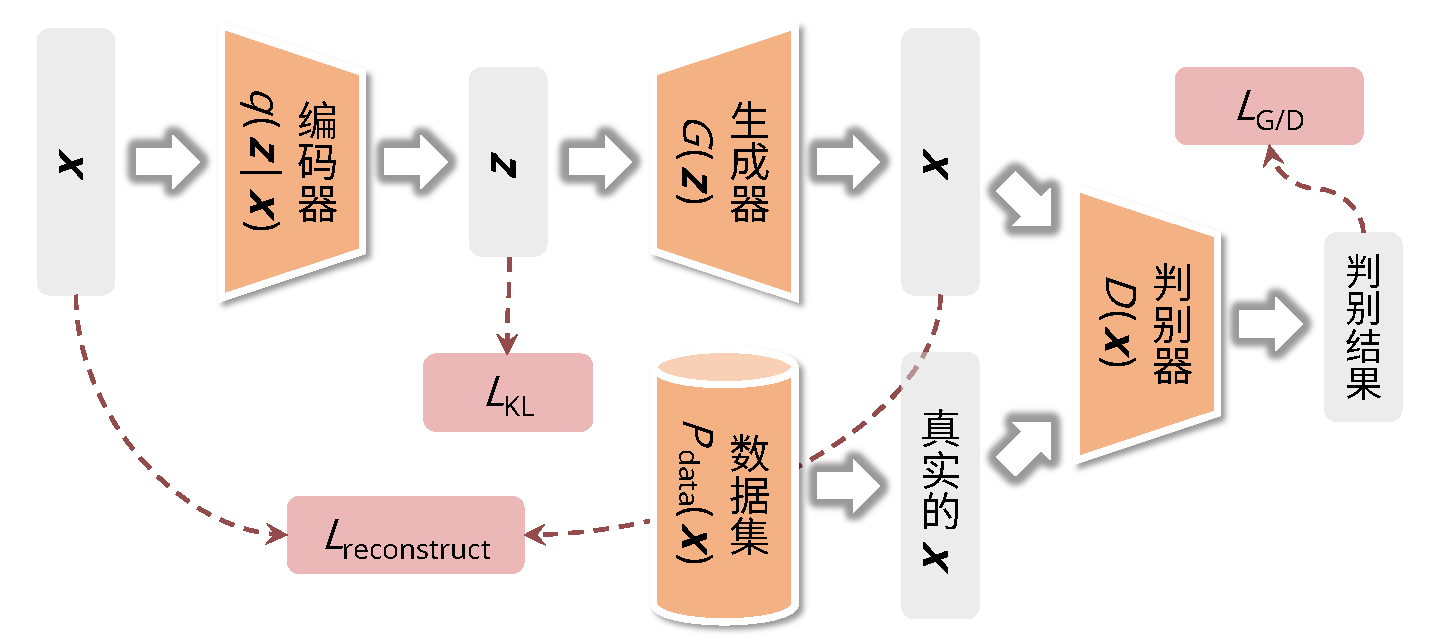
\includegraphics[width=.45\textwidth]{vaeganloss}}
	\caption{VAE/GAN\cite{vaegan}}
\end{figure}

与 VAE 和 GAN 类似,VAE/GAN 的损失函数包括三部分,分别为 KL 散度损失 $\Loss_{\text{KL}}$ 、 重建损失
$\Loss_{\text{reconstruct}}$ 以及 GAN 损失 $\Loss_{{G/D}}$:
\begin{subequations}
	\begin{align}
		\Loss_{\text{KL}}          & = \DKL{q(\bm z | \bm x; \bm\phi)}{p(\bm z)}
		\\
		\Loss_{\text{reconstruct}} & = \EXPECT{\bm z\sim q(\bm z | \bm x; \bm \phi)}{\left[\Norm*{\bm x - G(\bm z; \bm \theta)}^2\right]}
		\\
		\Loss_D                    & =
		- \EXPECT{\bm x \sim \PDATA(\bm x)}           \log(    D(\bm x))
		- \EXPECT{\bm z \sim \NormDist(\bm 0, \bm I)} \log(1 - D( G(\bm z)))
		\\
		\Loss_G                    & =
		- \EXPECT{\bm z \sim \NormDist(\bm 0, \bm I)} \log(D( G(\bm z)))
	\end{align}
	\label{eq:vaeganloss}
\end{subequations}
训练时,我们需要交替优化
\begin{subequations}
	\label{eq:vaegantrain}
	\begin{align}
		\bm\theta_D^*    & = \argmin{\bm\theta_D} = \lambda_D \cdot \Loss_D\label{eq:vaegantrain1}
		\\
		\bm\theta_\phi^* & = \argmin{\bm\theta_\phi} =
		\lambda_{\text{KL}} \cdot \Loss_{\text{KL}} +
		\lambda_{\text{reconstruct}} \cdot \Loss_{\text{reconstruct}}\label{eq:vaegantrain2}
		\\
		\bm\theta_G^*    & = \argmin{\bm\theta_G} =
		\lambda_G \cdot \Loss_G +
		\lambda_{\text{reconstruct}} \cdot \Loss_{\text{reconstruct}}\label{eq:vaegantrain3}
	\end{align}
\end{subequations}
其中 $\lambda_{\text{KL}}, \lambda_{\text{reconstruct}}, \lambda_D, \lambda_G$ 为平衡因子。
训练结束后,我们即丢弃判别器网络 $D$,与 GAN 的流程相同。


VAE/GAN 在图像生成任务上的表现如图 \ref{fig:vaegangen} 所示。
值得注意的是,由于编码器网络 $q(\bm z | \bm x)$ 可以
由数据 $\bm x$ 推出 $\bm z$ 的后验分布,因此 VAE/GAN 还可以用来
对图像进行重建或者去噪,如图  \ref{fig:vaeganrecon} 所示。
% 除了能生成图像外,GAN 还可以对图像进行插值。如图 \ref{fig:ganinter} 所示。
\begin{figure}[h]
	\centering%
	\subcaptionbox{图像生成\label{fig:vaegangen}}
	{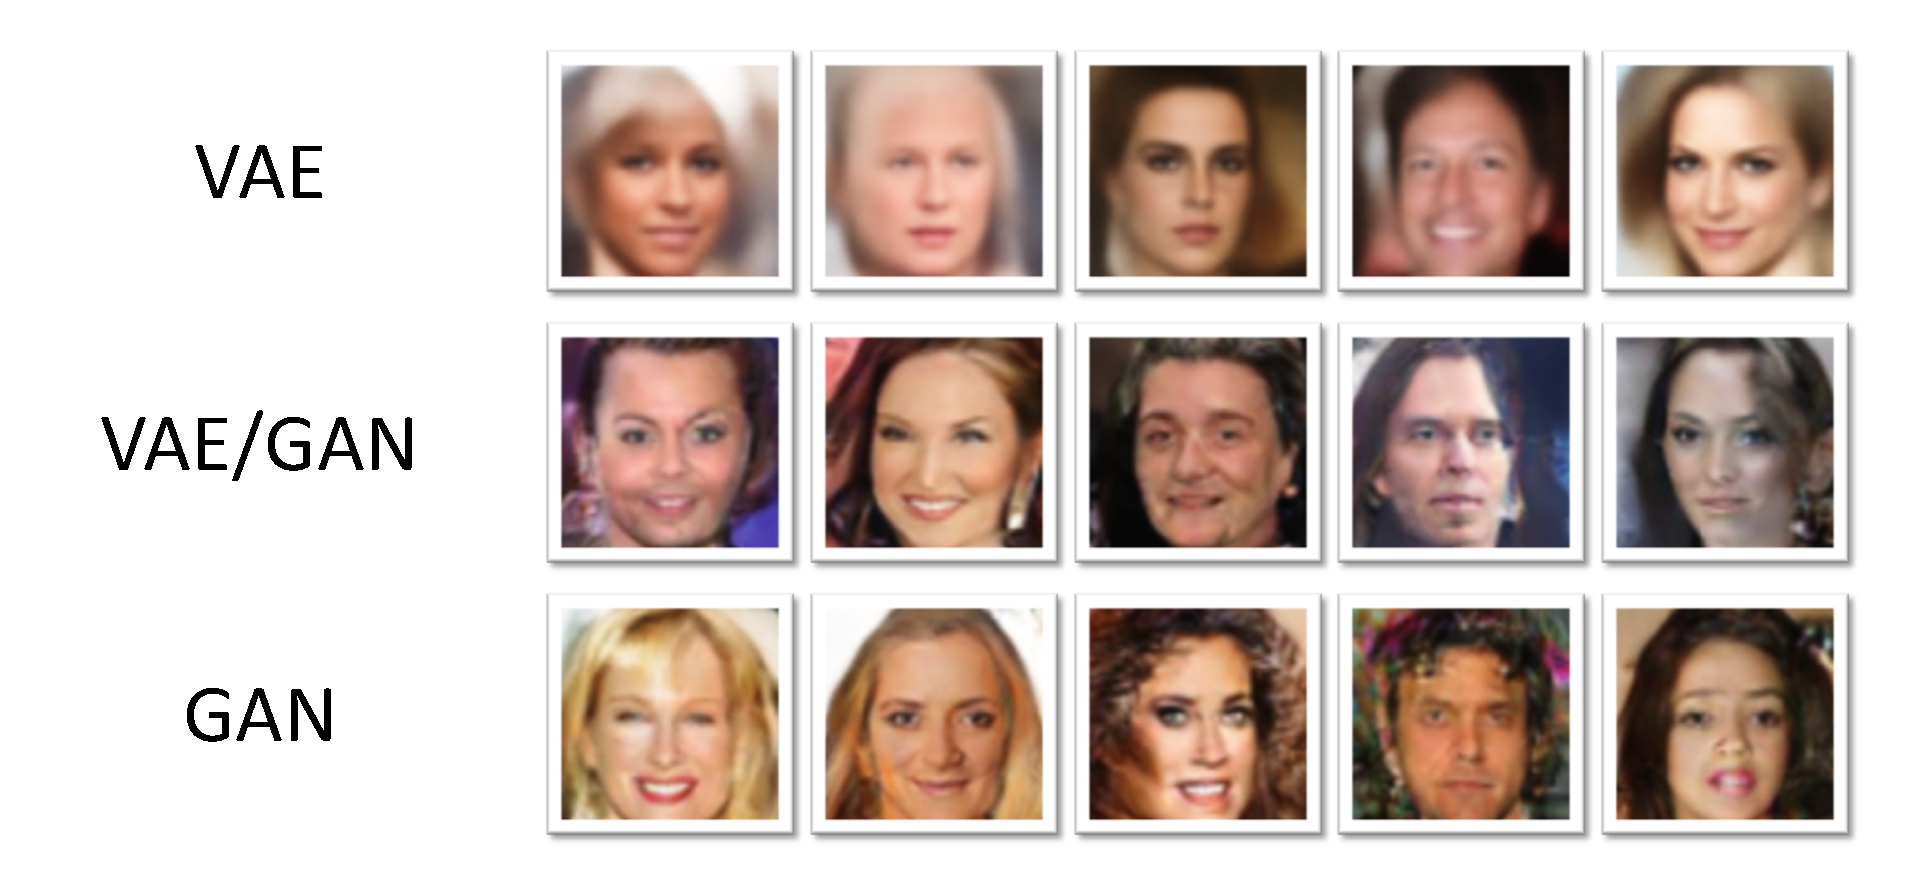
\includegraphics[width=.49\textwidth]{vaegangen}}%
	%\hspace{2em}%
	\subcaptionbox{图像重建/图像去噪\label{fig:vaeganrecon}}
	{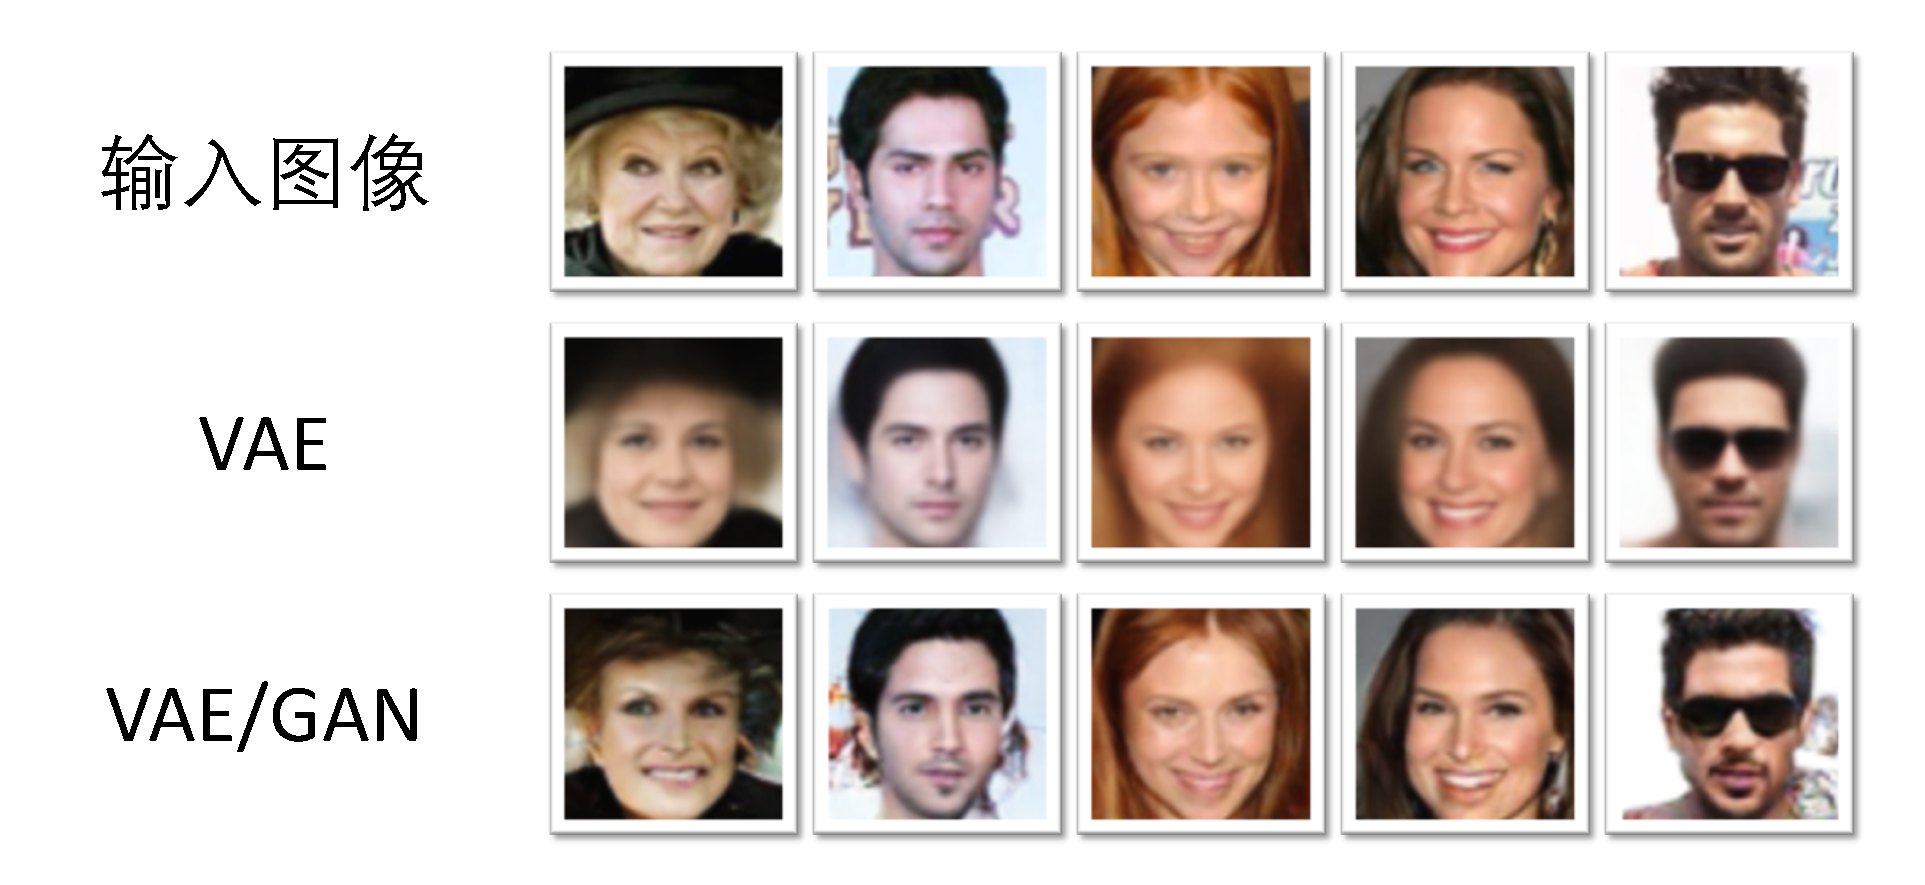
\includegraphics[width=.49\textwidth]{vaeganrecon}}
	\caption{使用 VAE/GAN 解决图像任务\cite{vaegan}}
\end{figure}

如果进一步在 VAE/GAN 中加入分类器,就可以得到 CVAE-GAN\cite{cvaegan}。它的表现效果更好,如图 \ref{fig:2dgen} 所示。限于篇幅,我们不再进一步展开介绍这个工作。




\section{基于点云的三维深度生成模型}
\label{section:gen3d}
在前面的章节中%第 \ref{cha:3d_deep_learning}、\ref{cha:gen} 章中,
我们先后介绍了点云三维深度学习和深度生成模型,并展示了这两个领域已有的丰硕的成果。
那么一个自然的问题是:
我们能否将深度生成模型在图像生成等任务上的良好表现%出的非凡成果
迁移到点云的生成任务上呢?
本节所介绍的工作 \inlinecite{latentpc} 正是在这个方向上的探索与尝试。 %这样的。在此方向上的尝试。%上做出了一定的尝试。

在介绍本节工作前,我们有必要对%本章以及第 \ref{cha:exp} 章的
记号的使用予以说明。
在前面的章节%第 \ref{cha:3d_deep_learning}、\ref{cha:gen} 章
中,我们曾用 $S = \{\bm p_i\}_{i=0}^{N - 1}
	= \{(x_i, y_i, z_i)^T\}_{i=0}^{N - 1}$ 表示点云数据,用
$\bm x$ 表示深度生成模型需要生成的数据。
而在本节和第 \ref{cha:exp}、\ref{cha:result} 章中,深度生成模型生成的数据恰好就是点云数据,因此我们将
视上下文算法的记号习惯,%灵活的
灵活地从 $\bm x$ 和 $S$ 中择一使用。但无论如何,这两者的本质是一样的。


\subsection{原始数据 GAN (Raw GAN, r-GAN) \label{section:rgan}}
一个直观的想法是:GAN 作为一个生成模型,其对于生成数据的形式没有任何假设。因此,我们可以
直接使用 %第 \ref{section:gan} 节中介绍的 
% GAN 来解决点云生成问题。%来完成点云生成的任务。
它解决点云生成问题。

正如我们在第 \ref{section:gan} 节介绍的, GAN 对于生成器网络 $G$ 和判别器网络 $D$ 的具体架构没有任何限定。
因此,为了使用 GAN,我们首先要因地制宜的设计好 $G$ 和 $D$ 的具体网络架构。
由于模型生成的对象是点云,因此我们可以参考第 \ref{cha:3d_deep_learning} 章中介绍的已有算法和网络架构。具体而言,
对于生成器网络 $S = G(\bm z; \bm \theta_G)$,第 $\ref{section:pointsetgen}$ 节中所介绍的 PointSetGen\cite{pointsetgen} 是一个不错的参考:我们可以借鉴 其 生成器部分,如全连接网络或者双分支网络。
而对于判别器网络 $D(S, \bm \theta_D)$,
我们可以直接使用第 $\ref{section:pointnet}$ 节中所介绍的 PointNet\cite{pointnet} 等架构。%能够出色的完成点云分类任务,因此。
固定了网络架构后,我们只要按照 GAN 的训练流程 \eqref{eq:ganloss0} 进行训练,就可以完成点云的生成任务。
我们将上述方法称为原始数据 GAN (Raw GAN, r-GAN)。

虽然 r-GAN 的流程直截了当,但它的实践效果并不好,如图 \ref{latent3drgan} 所示。
\begin{figure}[h]
	\centering%
	\subcaptionbox{真实数据\label{latent3dgt}}
	{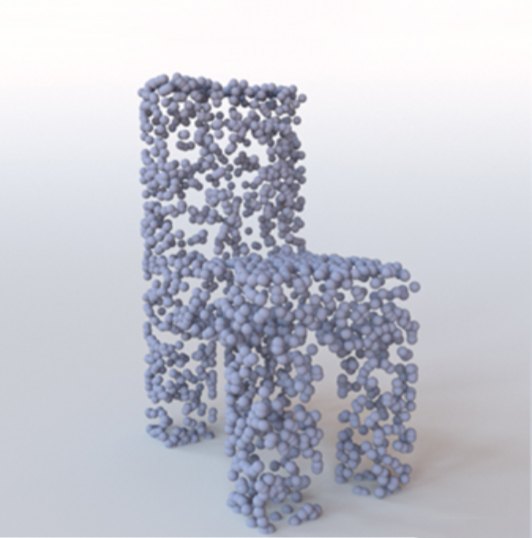
\includegraphics[width=.30\textwidth]{latent3dgt}}%
	\hspace{.5em}%
	\subcaptionbox{r-GAN\label{latent3drgan}}
	{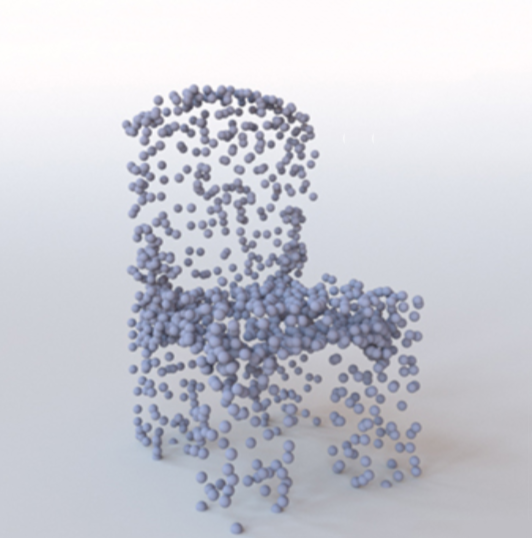
\includegraphics[width=.30\textwidth]{latent3drgan}}%
	\hspace{.5em}%
	\subcaptionbox{l-GAN\label{latent3dlgan}}
	{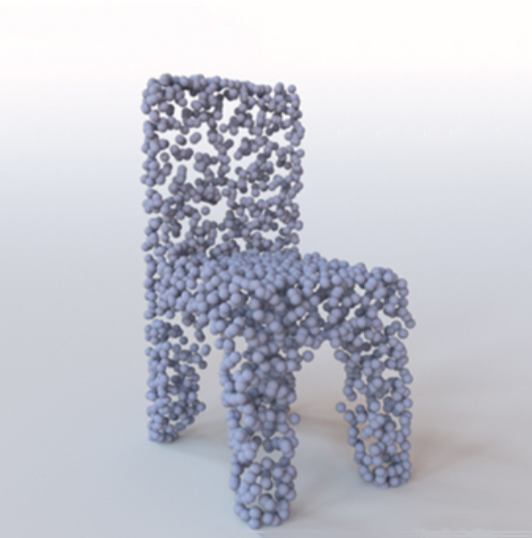
\includegraphics[width=.30\textwidth]{latent3dlgan}}%
	% \hspace{2em}%
	\caption{点云生成 \cite{latentpc}}
\end{figure}
在第 \ref{pointnet-robust} 节中,我们曾经介绍过 PointNet 的鲁棒性,即 PointNet 更关注点云数据的边、棱、角等关键信息,而忽略其他的非关键数据。
虽然这个性质有效提升了 PointNet 在点云分类、分割任务中的表现,但它对点云生成任务来说却是致命的。
%粗略地说,
粗略而言,在图 \ref{latent3drgan} 的例子中,椅子的棱角就是关键数据,而其内部点均为非关键数据。
由于 PointNet 会忽略掉非关键数据,因此作为判别器,它 %PointNet 
很难鉴定出椅面、椅背、椅子腿内部点的分布是否均匀合理,这也造成了图 \ref{latent3drgan} 中,点云集中在了某一区域如凳面上的问题。

\subsection{隐空间 GAN (Latent-space GAN, l-GAN)}
为了改善 r-GAN 的表现,我们可以先使用第 \ref{section:ae} 节中介绍的自编码器,提取点云的低维特征。

与 GAN 类似,自编码器同样是一种通用的模型,没有限制编码器 $E_{\text{AE}}$ 和解码器 $D_{\text{AE}}$ 的具体架构。
因此,我们%依然
同样可以取 $E_{\text{AE}}$ 为 PointNet,$D_{\text{AE}}$ 为 PointSetGen。而自编码器的损失函数 \eqref{eq:aeloss} 可以定义为点云的 Chamfer 距离 \eqref{eq:cd} 或推土机距离 \eqref{eq:emd}。
只要最小化此损失函数,我们就可以得到任意点云数据 $S = \bm x$ 的低维特征 $\bm z$。


然后,我们可以在点云的隐向量 $\bm z$ 上进行生成对抗训练,如图 \ref{fig:lgan} 所示。
\begin{figure}[h]
	\centering%
	{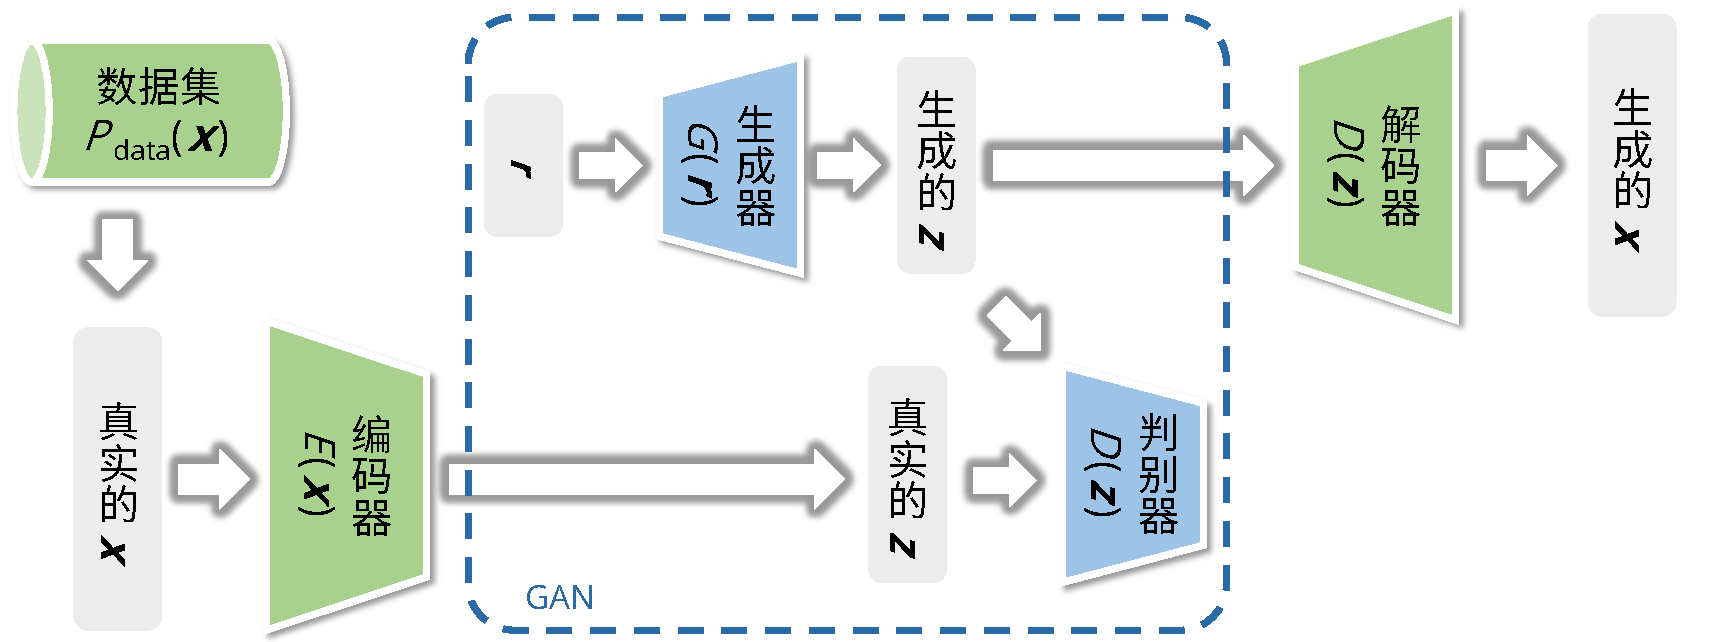
\includegraphics[width=.99\textwidth]{lgan}}%
	% \hspace{2em}%

	\caption{l-GAN 结构 \cite{latentpc}\label{fig:lgan}}
\end{figure}
我们认为:生成器从 $r \sim \NormDist(\bm 0, \bm I)$ 中生成隐向量 $\bm z = G_{\text{l-GAN}}(\bm r)$;
而判别器 $D_{\text{l-GAN}}(\bm z)$ 需要对于给定的隐向量 $\bm z$,判断它是从 $G_{\text{l-GAN}}$ 中生成的还是
从已有训练数据 $\bm x$ 提取的低维隐向量特征 $E_{\text{AE}}(\bm x)$。当需要从 $r \sim \NormDist(\bm 0, \bm I)$ 生成
实际的点云 $S = \bm x$时,我们需要经过生成器 $G_{\text{l-GAN}}$ 和解码器 $D_{\text{AE}}$ 两步映射:
\begin{align}
	S = \bm x = D_{\text{AE}}(\bm z) = D_{\text{AE}} \circ G_{\text{l-GAN}} (\bm r)
\end{align}
由于 GAN 生成的对象 $\bm z$ 已经是点云的低维特征了,因此我们而不必大费周章地再次使用 PointSetGen 和 PointNet 作为 $G_{\text{l-GAN}}$ 和 $D_{\text{l-GAN}}$ 的基本架构。事实上,仅使用简单的多层感知机,我们就%完全
可以达到较好的效果。
我们将上述方法称为隐空间 GAN (Latent-space GAN, l-GAN)。

l-GAN 在点云生成任务上的表现如 \ref{latent3dlgan} 所示,它解决了 PointNet 鲁棒性所带来的问题,质量较 r-GAN 相比有了一定的提升。


\subsection{Gauss 混合模型 (Gaussian Mixture Model, GMM)}
为了进一步提升生成点云的质量与覆盖率,工作 \inlinecite{latentpc} 还引入了隐向量 $\bm z$ 上的 Gauss 混合模型,作为 l-GAN 的改进版本。
但实验结果表明,与 l-GAN 相比,Gauss 混合模型的性能提升有限,其远远不如 r-GAN 到 l-GAN 的提升。%\cite{latentpc}。
限于篇幅原因,此处不再进一步展开介绍 Gauss 混合模型以及相关内容。%如何将其应用与三维点云生成的任务中。

% 与 r-GAN 相比,Gauss 混合模型的提升有限,同时不能很好地与 VAE/GAN 的工作结合,因此本文




% raw GAN

% l GAN
% 缺点,不能有效控制生成出的模型


\chapter{基于点云生成对抗网络的三维重建}
\label{cha:exp}
\section{动机}
在第 \ref{section:pointsetgen} 节中,我们详细地讨论了基于图片的三维点云重建算法 PointSetGen \cite{pointsetgen},% 工作
%的主要内容,
并指出了其两点不足:
\begin{itemize}
	\item 需要用户提供 mask 信息:用户体验差;
	\item 泛化能力差:对于训练数据集中未曾出现的新图像,PointSetGen 有可能失败。
\end{itemize}
本文工作的核心目标正是针对以上两点不足进行改进。

我们将在此章中详细地讲解与分析本工作的
%相关
算法流程与模型架构。
为了便于描述,我们首先定义本工作试图解决的问题。

\section{问题描述 \label{section:myquestion}}
在本工作中,用户需要提供的仅仅是一张三维物体的 RGB 图像 $\bm I$。%,且不含 mask 信息。
我们的目标之一是改善用户体验。因此,不像 PointSetGen,我们不再需要用户提供 mask 信息。

随后,算法需要根据用户提供的输入图像,以点云
$S = \{(x_i, y_i, z_i)^T\}_{i=0}^{N - 1}$
的形式重建出三维模型的完整结构,包括遮挡与不可见的部分。
为了简化问题,我们假设重建结果中点云的点数 $N$ 为固定常数 $N = \numprint{2048}$。
此处的 $N$ 是 PointSetGen 中的两倍,因为我们希望向用户呈现一个更稠密、更完整的重建结果。

此外,我们希望提升算法对于新数据的泛化能力,即相比于 PointSetGen,重建输出的质量应当得到增强。

更进一步的,我们还希望提升用户对于重建系统的可控制性。
具体而言,我们希望用户可以按照其期望,
对于多个已有的重建结果进行加权,让算法生成出一个介于它们之间的点云模型。
这样用户可以仅凭借较少的已有图像,就能自由地生成出期望的目标结果。


%物体检测与 mask 生成的 Mask R-CNN\cite{maskrcnn}、

% 生成 Mask

% 训练 AE

% 训练图像输入

% SN VAE GAN,具体


\section{模型架构}
在第 \ref{section:gan} 节中,我们领略了 GAN\cite{gan} “以假乱真”的高质量生成结果。
而在第 \ref{section:vaegan} 节中,我们也看到了 VAE/GAN\cite{vaegan} 在图像去噪等任务上的优异表现。
这些已有算法的特点正好与第 \ref{section:myquestion} 节中提出的%增强系统泛化能力和用户可控制性的
%任务
需求不谋而合,
启发了我们把 VAE/GAN 的工作引入到 PointSetGen 的想法。
与此同时,第 \ref{section:gen3d} 节的工作也提醒着我们:
尽可能避免直接在原始点云数据 $S = \bm x$ 上直接%使用
引入 GAN,而
%尽可能
使用其低维特征 $\bm z$ 代替。

\begin{figure}[h]
	\centering%
	{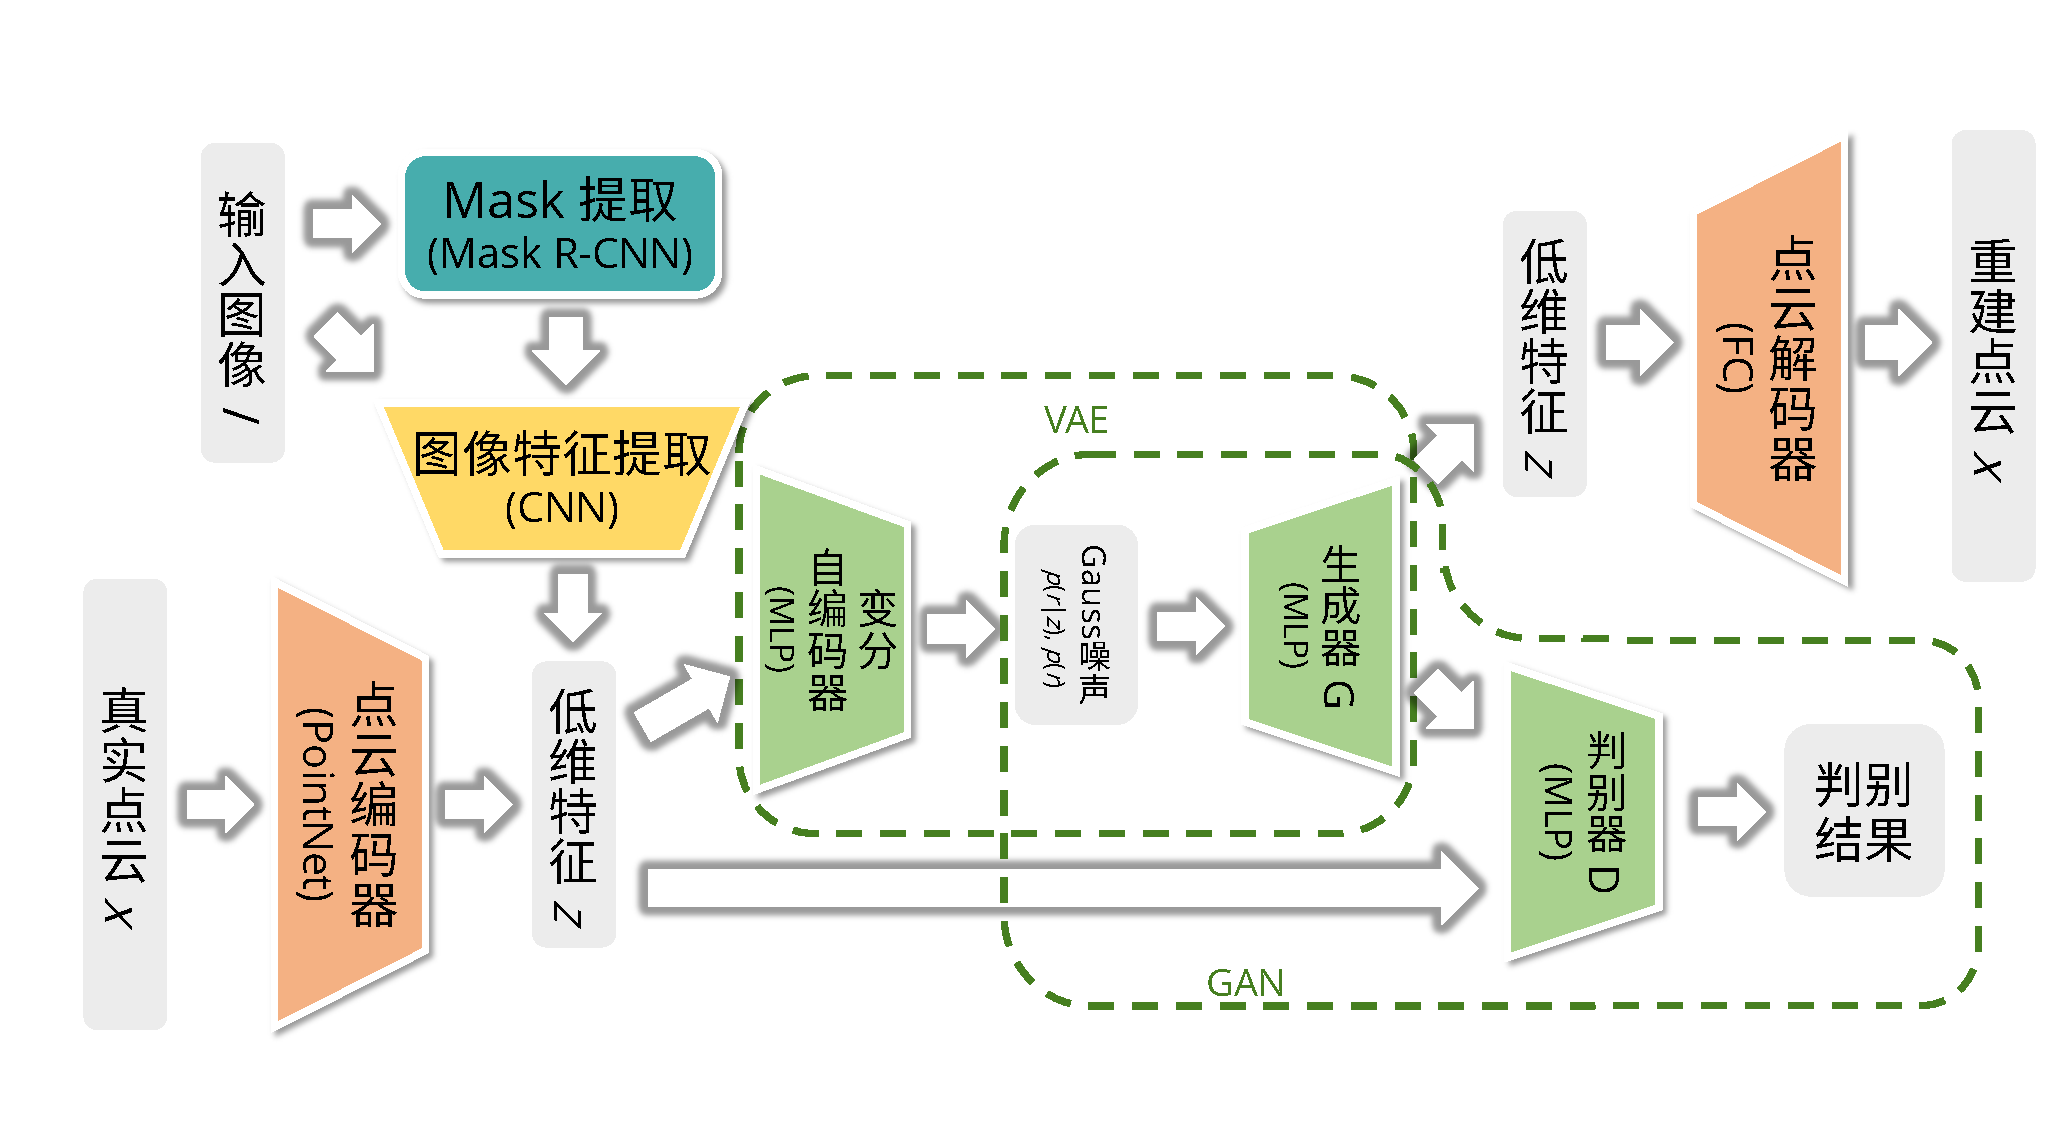
\includegraphics[width=.999\textwidth]{mystructure}}
	\caption{本工作的网络架构}
	\label{fig:mystructure}
\end{figure}

综上所述,为了解决第 \ref{section:myquestion} 节中提出的问题,我们使用如图 \ref{fig:mystructure} 所示
的%流水线
网络架构来处理用户的输入请求,%。%其中,
% 我们将各模块选取的网络架构标注在了右方。
其中,各模块所选取的具体%网络
架构被标注在了左方或下方位置。

% 要处理好做好流水线,
我们的%训练阶段
网络架构
% 主要
% 包括
%四个步骤
% 四部分
可以被粗略地分为四大组成部分
:点云自编码器(图 \ref{fig:mystructure} 橙红色部分)、Mask 生成模块(图 \ref{fig:mystructure} 青色部分)、图像特征提取模块(图 \ref{fig:mystructure} 黄色部分)以及 VAE/GAN(图 \ref{fig:mystructure} 绿色部分)。
我们将简要介绍这四部分的作用、目标及其%阶段%训练阶段%需要完成的任务
%的
训练方法。关于选取的模型架构与超参数的具体细节,请参见附录 \ref{cha:detail}。

\section{训练方法}
从图 \ref{fig:mystructure} 中可以看到,本工作的网络结构非常复杂。
事实上,本工作的训练过程也不是一步到位的,否则训练的代价太高;相反的,我们的训练过程按照模块的划分被分为四步。
本节介绍各模块的训练方法。
\subsection{点云自编码器\label{section:myae}}
点云自编码器 $E_{\text{AE}}, D_{\text{AE}}$ 对应图 \ref{fig:mystructure} 的橙红色部分。
它的核心目标是为了得到点云 $S = \bm x$ 的低维特征表示 $\bm z = E_{\text{AE}}(\bm x)$%。这样做的
。% 低维特征 $\bm z$ 
点云的低维特征 $\bm z$ 是后续训练流程所处理的基本对象。
%在后续训练的步骤中使用低维特征 $\bm z$ 的
相对于直接使用原始点云数据 $S = \bm x$,使用低维特征 $\bm z$ 有以下几点优势:
\begin{itemize}
	\item 能有效避免 PointNet\cite{pointnet} 鲁棒性带来的问题,%如同
	      正如
	      我们在第 \ref{section:rgan} 节中%所
	      提到的;%介绍的;
	\item 能有效加速后续步骤的运行速度,因为特征 $\bm z$ 的维数远远小于 $\bm x$ 的维数,后续步骤需要处理的数据规模大大降低;
	\item
	      % 提供了一个统一的标准,让图像提取模块可以和 VAE/GAN 结构自由对接。
	      能有效降低网络的复杂程度,减轻网络的负担:
	      例如,我们不必要求图像特征提取模块直接输出重建结果 $S = \bm x$,相反地,我们只要求它
	      % 只用
	      能够输出重建结果对应低维特征 $\bm z$ 即可。
	      重建出原始点云数据 $S$ 的任务将由解码器 $D_{\text{AE}}$ 进行进一步处理。
	      %否则,%若 GAN 的基本处理对象是点云,则

\end{itemize}

这个步骤只是一个预训练步骤,它的训练方法与第  \ref{section:gen3d} 节中 \inlinecite{latentpc} 工作提出的 l-GAN 如出一辙,此处不再赘述。
一旦预训练的过程完成,
%此训练步骤
%此步,
我们就固定编码器网络 $E_{\text{AE}}$ 和解码器网络 $D_{\text{AE}}$,并将特征
$\bm z = E_{\text{AE}}(\bm x)$ 视为数据集中的数据,不再考虑点云的原始表示 $\bm x$。

\subsection{Mask 生成模块 \label{my:mask}}
Mask 生成模块 $M$ 对应图 \ref{fig:mystructure} 的青色部分。
%此模块需要
其目的是
对用户提供的输入图像 $\bm I$ %上
进行物体分割,以自动生成出物体的 mask,使得后续的重建工作能够继续进行。

我们选择了 Mask R-CNN \cite{maskrcnn} 作为 mask 生成模块的网络架构。Mask R-CNN 是一个优秀的物体识别和语义分割算法,是早期工作 R-CNN\cite{rcnn}、Fast R-CNN\cite{fastrcnn}
、Faster R-CNN\cite{fasterrcnn} 的升级版本。相对于 Faster R-CNN,Mask R-CNN 增加了一个全卷积网络 (Fully Convolutional Network, FCN)分支,使得其能够胜任物体的分割任务。
由于物体检测和物体分割算法的具体实现并不是本文的讨论重点,因此我们不再单列章节%详细
展开介绍它们的具体细节和训练方法。%了。

在后期实验中,我们发现预训练好的 Mask R-CNN 对于小物体的分割非常准确,而对于大物体的分割就稍有欠缺了。%表现%就不那么好了。
究其原因,我们认为是其训练数据集%——
Microsoft Common Objects in Context (COCO) \cite{coco} 中小物体的数量远远多于大物体的数量%而
导致的。
而在本工作要解决的问题中,用户希望重建的物体是输入图像的主体,
其往往占据了整幅图像的绝大部分面积。这对于本工作而言是非常不利的。
% 往往会提供一张占据满整幅图像的

幸运的是,我们可以借助迁移学习的方法,提升 Mask R-CNN  在本问题上的表现。
具体而言,我们可以对于每一类物体,收集约 100 张占图像面积比例较高的大物体照片,
并手工标注其真实的 mask。利用这些新数据,我们在预训练好的 Mask R-CNN 进一步%继续
训练,直到 Mask R-CNN 能够比较好地完成大物体的分割任务为止。

\subsection{图像特征提取模块}
图像特征提取模块 $E_{\text{Image}}$ 对应图 \ref{fig:mystructure} 的绿色部分。
它的核心目标是:根据输入的 RGB 图像 $\bm I$ 和 mask $M(\bm I)$,计算图中三维模型点云表示 %$\bm x$ 
的低维特征 $\bm z = E_{\text{Image}}(\bm I_k, M(\bm I_k); \theta_{\text{Image}})$,以实现和 VAE/GAN\cite{vaegan} 以及解码器 $D_{\text{AE}}$ 的对接。
% 后面我们将会看到,
% 我们马上就可以
我们将会看到:
一旦特征 $\bm z$ 被计算出来,我们就可以使用 VAE/GAN 对其降噪,从而计算出一个更好的特征 $\bm z^*$,正如我们在第 \ref{section:vaegan} 节中所介绍的一样。
%此特征
经过%点云自编码器的
解码器 $D_{\text{AE}}$ 对此特征的进一步映射后,%后,%我们就可以得到
我们就得到了质量较好的重建结果 $S^* = \bm x^* = D_{\text{AE}}(\bm z^*)$。
这个点云降噪过程实现了%第 \ref{section:myquestion} 节中
提升重建模型质量 的基本要求。
% 这实现了 在第 \ref{section:myquestion} 节中 提出的提升重建模型质量 的基本要求。

% 正如在第 \ref{section:myae} 节中我们所强调的,图像特征提取模块不会涉及到任何点云原始数据 $\bm x$ 的计算,所有点云数据都是以其低维特征 $\bm z$ 的形式表现的。

在本工作中,图像特征提取模块的核心架构是卷积神经网络。这样的设计与 PointSetGen 是一脉相承的。由于卷积神经网络并不是本文介绍的重点,故其
具体细节此处不再赘述。

在训练时,我们希望最小化与模块输出与实际点云低维特征 $\bm z_{\text{gt}} = E_{\text{AE}}(\bm x_{\text{gt}})$ 之间的距离。即,对于数据集中的所有的图像 $\bm I$ 及其标注的真实点云 $\bm x_{\text{gt}} = S_{\text{gt}}$,我们希望最小化
\begin{align}
	\Loss(\bm \theta_{\text{Image}}) = \sum_k
	\Norm*{E_{\text{Image}}(\bm I_k, M(\bm I_k); \theta_{\text{Image}}) -
		E_{\text{AE}}(\bm x_{\text{gt}, k})}^2
	\label{eq:myimloss}
\end{align}
其中 $k$ 表示数据编号。

\subsection{VAE/GAN}
VAE/GAN 对应图 \ref{fig:mystructure} 的黄色部分,
包括了变分自编码器 $q(\bm r | \bm z; \bm\phi)$、
判别器 $D_{\text{GAN}}(\bm z)$、
生成器 $G_{\text{GAN}}(\bm r)$ 三部分。

通过第 \ref{section:gan} 、 \ref{section:vaegan} 节 的介绍,我们了解了 VAE/GAN\cite{vaegan}可以对图像进行插值和降噪。因此,我们把 VAE/GAN 引入到这个重建问题中,
并希望它能够实现增强重建质量与提升用户可控性这两点需求。%,如图\ref{section:myquestion}。

此处 VAE/GAN 的损失函数和训练方法与我们在第 \ref{section:vaegan} 节中介绍的 VAE/GAN 是基本类似的。
由于此处生成器 $G_{\text{GAN}}$ 从隐向量 $\bm r \sim \NormDist(\bm0, \bm I)$ 直接生成特征 $\bm z$,因此我们可以仿照 式 \eqref{eq:vaeganloss} 定义损失函数:
\begin{subequations}
	\label{eq:myvaeganloss}
	\begin{align}
		\Loss_{\text{KL}}          & = \DKL{q(\bm r | \bm z; \bm\phi)}{p(\bm r)}
		\\
		\Loss_{\text{reconstruct}} & = \EXPECT{\bm r\sim q(\bm r | \bm z; \bm \phi)}{\left[\Norm*{\bm z - G_{\text{GAN}}(\bm r)}^2\right]}
		\\
		\Loss_D                    & =
		- \EXPECT{\bm z \sim \PDATA(\bm z)}           \log(    D_{\text{GAN}}(\bm z))
		- \EXPECT{\bm r \sim \NormDist(\bm 0, \bm I)} \log(1 - D_{\text{GAN}}( G_{\text{GAN}}(\bm r)))
		\\
		\Loss_G                    & =
		- \EXPECT{\bm r \sim \NormDist(\bm 0, \bm I)} \log(D_{\text{GAN}}( G_{\text{GAN}}(\bm r)))
	\end{align}
\end{subequations}
而训练方法没有任何变化,仍然是交替优化:
\begin{subequations}
	\begin{align}
		\bm\theta_D^*    & = \argmin{\bm\theta_D} = \lambda_D \cdot \Loss_D \tag*{\ref{eq:vaegantrain1}}
		\\
		\bm\theta_\phi^* & = \argmin{\bm\theta_\phi} =
		\lambda_{\text{KL}} \cdot \Loss_{\text{KL}} +
		\lambda_{\text{reconstruct}} \cdot \Loss_{\text{reconstruct}} \tag*{\ref{eq:vaegantrain2}}
		\\
		\bm\theta_G^*    & = \argmin{\bm\theta_G} =
		\lambda_G \cdot \Loss_G +
		\lambda_{\text{reconstruct}} \cdot \Loss_{\text{reconstruct}} \tag*{\ref{eq:vaegantrain3}}
	\end{align}
\end{subequations}
其中 $\lambda_{\text{KL}}, \lambda_{\text{reconstruct}}, \lambda_D, \lambda_G$ 为平衡因子。

在第 \ref{section:gan}、\ref{section:ganimprove} 节中,我们介绍了经典 GAN 存在不稳定、训练困难的问题。
为了避免这种情况的发生,这里我们使用了谱标准化生成对抗网络 (Spectral Normalization Generative Adversarial Network, SNGAN)
\cite{sngan}。SNGAN 通过
限制判定器网络中每一层的谱半径
%单位化
为 $1$,有效地确保了 $D_{\text{GAN}}$ 满足 Lipschitz 连续条件 \eqref{eq:lip},增强了 GAN 训练过程的稳定性,且其速度优于其他试图改进 GAN 的工作。
限于篇幅,此处不再进一步展开介绍 SNGAN 及其相关工作。

% $\Norm{D_{\text{GAN}}}_{\text{Lip}} \le 1$,
% 其结构正是我们在


\chapter{实验结果}
\label{cha:result}

\section{数据集的准备 \label{section:mypre}}
在第 \ref{section:pointsetgenpre} 节中,我们介绍了 PointSetGen
使用 RenderForCNN\cite{rendercnn} 的方法,通过计算机图形学中的渲染手段,获取图像训练数据。
但通过观察 PointSetGen 的实现,我们发现了其数据集的准备工作有一定的不足:
\begin{itemize}
	\item 仰角与距离固定:渲染时固定了摄像机的仰角为 $20^\circ$,%摄像机
	      到物体的距离为 $2.5$ 倍物体半径。这使得 PointSetGen 不能适应新的摄像机视角与距离;
	\item 标注与视角相关:标注的真实点云数据是相对于相机坐标系的。这会使得标注点云随着摄像机视角的旋转而转动。
	      由于网络的核心任务是重建而非视角估计,因此,这样的转动在一定程度上是噪音,不利于网络把握三维模型在几何形状上的规律;
	\item 模型视角少:每个模型渲染的视角数较少,没有充分利用已有数据的信息;
	\item 背景色固定:渲染出的图像中,背景色的不透明度 (Alpha) 通道被设为了 0,但颜色 (RGB) 通道 被设为了固定常数。此处的 RGB 值虽然没有意义,但它仍然参与了网络的计算,影响着输出结果。
\end{itemize}
对此,我们使用如下的新策略,重新对 ShapeNet\cite{shapenet} 进行了渲染,从而完成了数据集的准备工作:
\begin{itemize}
	\item 视角随机化:使得摄像机的仰角从 $20^\circ$ 到 $60^\circ$ 间均匀分布,方向角从 $0^\circ$ 到 $360^\circ$ 间均匀分布,因为这基本上涵盖了人类摄影的常见角度;

	\item 距离随机化:使得摄像机到物体的距离从 $1.7$ 倍物体半径到 $2.5$ 倍物体半径间均匀分布。过远或者过近会使得物体过大或者过小,不利于重建;

	\item 光照随机化:引入 3 到 10 个不等的点光源,其位置、亮度均随机,用于模拟各种强弱光环境;

	\item 标注与视角无关:标注的真实点云数据使用局部坐标系,其不会随着视角的变化而转动,利于网络
	      %的
	      学习出三维模型的几何分布规律;

	\item 多视角渲染:每个模型渲染 100 个不同的视角,充分挖掘已有的数据;

	\item 背景色随机化:背景色设置为 Alpha 通道为 0,但 RGB 通道为随机值的颜色。
	      这使得网络的输出尽可能不受背景色 RGB 值的影响。
\end{itemize}

表格 \ref{tab:render} 展示了 PointSetGen 所渲染的数据集与本工作所渲染的数据集的差别。
可以看到,与 PointSetGen 相比,本工作渲染的数据集质量更高,视角更多,光照变化也更丰富,
具更适合做为训练网络的数据。

\begin{table}[htb]
	\centering
	\caption{PointSetGen\cite{pointsetgen} 与 本工作渲染的数据集(部分)\label{tab:render}}
	\begin{tabularx}{\linewidth}{ccc}
		\toprule[1.5pt]
		{\heiti PSG\cite{pointsetgen}}                     &  & {\heiti 本工作}
		\\\midrule[1pt]
		{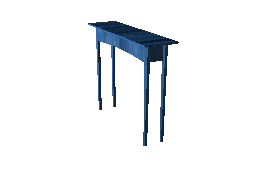
\includegraphics[width=.145\textwidth]{data/1/a}} &  &
		{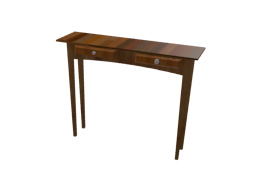
\includegraphics[width=.145\textwidth]{data/1/1}}
			{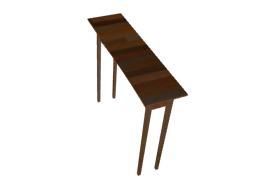
\includegraphics[width=.145\textwidth]{data/1/2}}
			{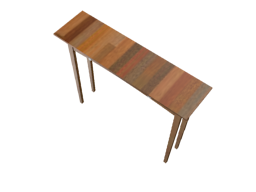
\includegraphics[width=.145\textwidth]{data/1/3}}
			{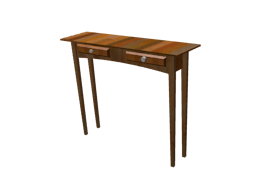
\includegraphics[width=.145\textwidth]{data/1/4}}
			{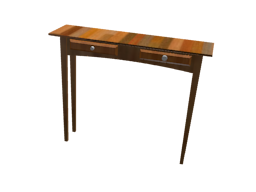
\includegraphics[width=.145\textwidth]{data/1/5}}
		\\
		{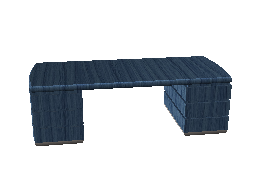
\includegraphics[width=.145\textwidth]{data/2/a}} &  &
		{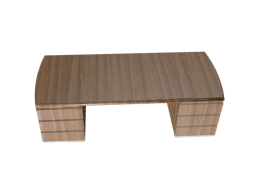
\includegraphics[width=.145\textwidth]{data/2/1}}
			{\includegraphics[width=.145\textwidth]{data/2/2}}
			{\includegraphics[width=.145\textwidth]{data/2/3}}
			{\includegraphics[width=.145\textwidth]{data/2/4}}
			{\includegraphics[width=.145\textwidth]{data/2/5}}
		\\
		{\includegraphics[width=.145\textwidth]{data/3/a}} &  &
		{\includegraphics[width=.145\textwidth]{data/3/1}}
			{\includegraphics[width=.145\textwidth]{data/3/2}}
			{\includegraphics[width=.145\textwidth]{data/3/3}}
			{\includegraphics[width=.145\textwidth]{data/3/4}}
			{\includegraphics[width=.145\textwidth]{data/3/5}}
		\\
		{\includegraphics[width=.145\textwidth]{data/4/a}} &  &
		{\includegraphics[width=.145\textwidth]{data/4/1}}
			{\includegraphics[width=.145\textwidth]{data/4/2}}
			{\includegraphics[width=.145\textwidth]{data/4/3}}
			{\includegraphics[width=.145\textwidth]{data/4/4}}
			{\includegraphics[width=.145\textwidth]{data/4/5}}
		\\
		{\includegraphics[width=.145\textwidth]{data/5/a}} &  &
		{\includegraphics[width=.145\textwidth]{data/5/1}}
			{\includegraphics[width=.145\textwidth]{data/5/2}}
			{\includegraphics[width=.145\textwidth]{data/5/3}}
			{\includegraphics[width=.145\textwidth]{data/5/4}}
			{\includegraphics[width=.145\textwidth]{data/5/5}}
		\\
		\bottomrule[1.5pt]
	\end{tabularx}
\end{table}


% 实验结果

% Mask 表现

\section{Mask 提取与三维重建结果}
为了分别展现各个模块的质量,在本节中我们暂时假设:对于重建任务,算法已经得到了精确的 mask。
\subsection{Mask 提取\label{section:mask}}
正如第 \ref{my:mask} 节中所介绍的,我们希望手动标注各种大物体的 mask,作为训练数据集和测试数据集,对 Mask R-CNN 做迁移学习的训练。

然而标注 mask 任务通常很繁杂。由于时间有限,因此我们仅仅对少量的物体进行了测试。

迁移学习前后,模型给出的 mask 如图 \ref{fig:transferchange} 所示。可以看到,通过迁移学习,mask 的质量有了很大的提升。
\begin{figure}[h]
	\centering%
	\subcaptionbox{迁移学习前}
	{\includegraphics[width=.45\textwidth]{mask/mugori3}}%
	\hspace{2em}%
	\subcaptionbox{迁移学习后}
	{\includegraphics[width=.45\textwidth]{mask/mugreal3}}
	\caption{迁移学习对于 mask 的改善\label{fig:transferchange}}
\end{figure}

而迁移学习后的新网络在测试数据集上的表现 % 给出 Mask 
如图 \ref{fig:transfertest} 所示。
\begin{figure}[h]
	\centering%
	{\includegraphics[width=.23\textwidth]{mask/mug1}}
	{\includegraphics[width=.23\textwidth]{mask/mug2}}
	{\includegraphics[width=.23\textwidth]{mask/mug3}}
	{\includegraphics[width=.23\textwidth]{mask/mug4}}
	\caption{迁移学习后的 Mask R-CNN \cite{maskrcnn} 在测试集上的表现\label{fig:transfertest}}
\end{figure}

虽然我们没有在更多的类别上进行更广泛的测试,但我们相信,在迁移学习的指引下,预训练的模型与后期新标注的数据必将相辅相成,共同促进 mask 的质量%一定可以得到
的进一步提升。

% 重建表现

\subsection{三维重建 \label{section:recon}}

\newcounter{themenumber}
\newcounter{themenumber2}

我们首先使用 PointSetGen 工作的测试集,
对本工作和 PointSetGen 进行了实验,结果如表 \ref{tab:reconpsgdata} 所示。
对比两工作的重建结果,我们发现:虽然 PointSetGen 在原有的数据集上的重建结果尚可,%还可以被接受,
但本工作重建出的点云更稠密,更完整,而且对于几何形状的把握也明显的优于 PointSetGen。


\begin{longtable}[c]{c*{5}{c}}
	\caption{
		PointSetGen\cite{pointsetgen} 与本工作在 PointSetGen 测试集上的表现(部分)\label{tab:reconpsgdata}}                                      \\

	\toprule[1.5pt]
	{输入 $\bm I$}                                                                       & {\heiti 本工作} & {\heiti PSG\cite{pointsetgen}} &
	{输入 $\bm I$}                                                                       & {\heiti 本工作} & {\heiti PSG\cite{pointsetgen}}
	\\\midrule[1pt]
	\endfirsthead
	\multicolumn{6}{c}{续表~\thetable \hskip1em
		PointSetGen\cite{pointsetgen} 与本工作在 PointSetGen 测试集上的表现(部分)}                                                              \\
	\toprule[1.5pt]
	{输入 $\bm I$}                                                                       & {\heiti 本工作} & {\heiti PSG\cite{pointsetgen}} &
	{输入 $\bm I$}                                                                       & {\heiti 本工作} & {\heiti PSG\cite{pointsetgen}}
	\\\midrule[1pt]

	\endhead
	\bottomrule[1.5pt] %\hline
	\multicolumn{6}{r}{续下页}
	\endfoot
	\endlastfoot
	\forloop[2]{themenumber}{0}{\value{themenumber} < 32}
	{
		\setcounter{themenumber2}{\value{themenumber}}\addtocounter{themenumber2}{1}

	{\includegraphics[width=.14\textwidth]{cmp_psgdata/chair_\arabic{themenumber}}}      &
	{\includegraphics[width=.14\textwidth]{cmp_psgdata/our_chair_\arabic{themenumber}}}  &
	{\includegraphics[width=.14\textwidth]{cmp_psgdata/psg_chair_\arabic{themenumber}}}  &
	{\includegraphics[width=.14\textwidth]{cmp_psgdata/chair_\arabic{themenumber2}}}     &
	{\includegraphics[width=.14\textwidth]{cmp_psgdata/our_chair_\arabic{themenumber2}}} &
		{\includegraphics[width=.14\textwidth]{cmp_psgdata/psg_chair_\arabic{themenumber2}}}
		\\
	}

	\forloop[2]{themenumber}{0}{\value{themenumber} < 18}
	{
		\setcounter{themenumber2}{\value{themenumber}}\addtocounter{themenumber2}{1}

	{\includegraphics[width=.14\textwidth]{cmp_psgdata/car_\arabic{themenumber}}}        &
	{\includegraphics[width=.14\textwidth]{cmp_psgdata/our_car_\arabic{themenumber}}}    &
	{\includegraphics[width=.14\textwidth]{cmp_psgdata/psg_car_\arabic{themenumber}}}    &
	{\includegraphics[width=.14\textwidth]{cmp_psgdata/car_\arabic{themenumber2}}}       &
	{\includegraphics[width=.14\textwidth]{cmp_psgdata/our_car_\arabic{themenumber2}}}   &
		{\includegraphics[width=.14\textwidth]{cmp_psgdata/psg_car_\arabic{themenumber2}}}
		\\
	}

	\setcounter{themenumber2}{\value{themenumber}}\addtocounter{themenumber2}{1}

	{\includegraphics[width=.14\textwidth]{cmp_psgdata/car_\arabic{themenumber}}}        &
	{\includegraphics[width=.14\textwidth]{cmp_psgdata/our_car_\arabic{themenumber}}}    &
	{\includegraphics[width=.14\textwidth]{cmp_psgdata/psg_car_\arabic{themenumber}}}    &
	{\includegraphics[width=.14\textwidth]{cmp_psgdata/car_\arabic{themenumber2}}}       &
	{\includegraphics[width=.14\textwidth]{cmp_psgdata/our_car_\arabic{themenumber2}}}   &
	{\includegraphics[width=.14\textwidth]{cmp_psgdata/psg_car_\arabic{themenumber2}}}

	\\
	\bottomrule[1.5pt]
\end{longtable}







随后,我们还使用了本文的测试数据集,对两工作进行了测试,如表 \ref{tab:recon} 所示。
% 使用了第 \ref{section:mypre} 节中
% 介绍的增强数据集 %新数据集
% 详细讨论过
% 介绍的
% 增强数据集,取出其测试集,对两工作进行测试,如表 \ref{tab:recon} 所示。
%上 %中的测试集上
对比 PointSetGen 和本工作的重建结果,我们可以明显地看到 PointSetGen 在新数据上的表现很差,
因为训练 PointSetGen 所使用的训练数据集有缺陷,我们在第 \ref{section:mypre} 节中已有所提及。
而在本工作中,我们不仅使用了 VAE/GAN 保证了其重建质量
,还使用了增强后的新数据集进行训练,大大提高了网络的泛化能力,因此重建质量要明显优于 PointSetGen。


\begin{longtable}[c]{c*{5}{c}}
	\caption{
		PointSetGen\cite{pointsetgen} 与 本工作 在 本文测试集上的表现(部分)\label{tab:recon}}                                           \\

	\toprule[1.5pt]
	{输入 $\bm I$}                                                               & {\heiti 本工作} & {\heiti PSG\cite{pointsetgen}} &
	{输入 $\bm I$}                                                               & {\heiti 本工作} & {\heiti PSG\cite{pointsetgen}}
	\\\midrule[1pt]
	\endfirsthead
	\multicolumn{6}{c}{续表~\thetable \hskip1em
		PointSetGen\cite{pointsetgen}  与 本工作 在 本文测试集上的表现(部分)}                                                           \\
	\toprule[1.5pt]
	{输入 $\bm I$}                                                               & {\heiti 本工作} & {\heiti PSG\cite{pointsetgen}} &
	{输入 $\bm I$}                                                               & {\heiti 本工作} & {\heiti PSG\cite{pointsetgen}}
	\\\midrule[1pt]


	\endhead
	\bottomrule[1.5pt] %\hline
	\multicolumn{6}{r}{续下页}
	\endfoot
	\endlastfoot
	% \forloop{themenumber}{1}{\value{themenumber} < 31}
	% {
	% {\includegraphics[width=.14\textwidth]{cmp/car_\arabic{themenumber}}}&
	% {\includegraphics[width=.14\textwidth]{cmp/our_car_\arabic{themenumber}}}&
	% {\includegraphics[width=.14\textwidth]{cmp/psg_car_\arabic{themenumber}}}&
	% {\includegraphics[width=.14\textwidth]{cmp/chair_\arabic{themenumber}}}&
	% {\includegraphics[width=.14\textwidth]{cmp/our_chair_\arabic{themenumber}}}&
	% {\includegraphics[width=.14\textwidth]{cmp/psg_chair_\arabic{themenumber}}}
	% \\
	% }
	% {\includegraphics[width=.14\textwidth]{cmp/car_\arabic{themenumber}}}&
	% {\includegraphics[width=.14\textwidth]{cmp/our_car_\arabic{themenumber}}}&
	% {\includegraphics[width=.14\textwidth]{cmp/psg_car_\arabic{themenumber}}}&
	% {\includegraphics[width=.14\textwidth]{cmp/chair_\arabic{themenumber}}}&
	% {\includegraphics[width=.14\textwidth]{cmp/our_chair_\arabic{themenumber}}}&
	% {\includegraphics[width=.14\textwidth]{cmp/psg_chair_\arabic{themenumber}}}
	% \\
	\forloop[2]{themenumber}{0}{\value{themenumber} < 32}
	{
		\setcounter{themenumber2}{\value{themenumber}}\addtocounter{themenumber2}{1}

	{\includegraphics[width=.14\textwidth]{cmp/chair_\arabic{themenumber}}}      &
	{\includegraphics[width=.14\textwidth]{cmp/our_chair_\arabic{themenumber}}}  &
	{\includegraphics[width=.14\textwidth]{cmp/psg_chair_\arabic{themenumber}}}  &
	{\includegraphics[width=.14\textwidth]{cmp/chair_\arabic{themenumber2}}}     &
	{\includegraphics[width=.14\textwidth]{cmp/our_chair_\arabic{themenumber2}}} &
		{\includegraphics[width=.14\textwidth]{cmp/psg_chair_\arabic{themenumber2}}}
		\\
	}
	\forloop[2]{themenumber}{0}{\value{themenumber} < 30}
	{
		\setcounter{themenumber2}{\value{themenumber}}\addtocounter{themenumber2}{1}

	{\includegraphics[width=.14\textwidth]{cmp/car_\arabic{themenumber}}}        &
	{\includegraphics[width=.14\textwidth]{cmp/our_car_\arabic{themenumber}}}    &
	{\includegraphics[width=.14\textwidth]{cmp/psg_car_\arabic{themenumber}}}    &
	{\includegraphics[width=.14\textwidth]{cmp/car_\arabic{themenumber2}}}       &
	{\includegraphics[width=.14\textwidth]{cmp/our_car_\arabic{themenumber2}}}   &
		{\includegraphics[width=.14\textwidth]{cmp/psg_car_\arabic{themenumber2}}}
		\\
	}
	\setcounter{themenumber2}{\value{themenumber}}\addtocounter{themenumber2}{1}

	{\includegraphics[width=.14\textwidth]{cmp/car_\arabic{themenumber}}}        &
	{\includegraphics[width=.14\textwidth]{cmp/our_car_\arabic{themenumber}}}    &
	{\includegraphics[width=.14\textwidth]{cmp/psg_car_\arabic{themenumber}}}    &
	{\includegraphics[width=.14\textwidth]{cmp/car_\arabic{themenumber2}}}       &
	{\includegraphics[width=.14\textwidth]{cmp/our_car_\arabic{themenumber2}}}   &
	{\includegraphics[width=.14\textwidth]{cmp/psg_car_\arabic{themenumber2}}}
	\\
	\bottomrule[1.5pt]
\end{longtable}






此外,我们还测试了从真实照片中重建的情况,如表 \ref{tab:realimg} 所示。

\begin{longtable}[c]{c*{2}{c}}
	\caption{
		PointSetGen\cite{pointsetgen} 与 本工作 在真实照片中的表现(部分)\label{tab:realimg}}                     \\
	\toprule[1.5pt]
	{输入 $\bm I$}                                          & {\heiti 本工作} & {\heiti PSG\cite{pointsetgen}}
	\\\midrule[1pt]
	\endfirsthead
	\multicolumn{3}{c}{续表~\thetable \hskip1em
		PointSetGen\cite{pointsetgen} 与 本工作 在真实照片中的表现(部分)}                                        \\
	\toprule[1.5pt]
	{输入 $\bm I$}                                          & {\heiti 本工作} & {\heiti PSG\cite{pointsetgen}}
	\\\midrule[1pt]
	\endhead
	\bottomrule[1.5pt] %\hline
	\multicolumn{3}{r}{续下页}
	\endfoot
	\endlastfoot

	{\includegraphics[width=.32\textwidth]{cmp/car1}}       &
	{\includegraphics[width=.32\textwidth]{cmp/car1_our}}   &
	{\includegraphics[width=.32\textwidth]{cmp/car1_psg}}
	\\
	{\includegraphics[width=.30\textwidth]{cmp/car2}}       &
	{\includegraphics[width=.30\textwidth]{cmp/car2_our}}   &
	{\includegraphics[width=.30\textwidth]{cmp/car2_psg}}
	\\
	{\includegraphics[width=.30\textwidth]{cmp/car3}}       &
	{\includegraphics[width=.30\textwidth]{cmp/car3_our}}   &
	{\includegraphics[width=.30\textwidth]{cmp/car3_psg}}
	\\
	{\includegraphics[width=.30\textwidth]{cmp/chair1}}     &
	{\includegraphics[width=.30\textwidth]{cmp/chair1_our}} &
	{\includegraphics[width=.30\textwidth]{cmp/chair1_psg}}
	\\
	{\includegraphics[width=.30\textwidth]{cmp/chair2}}     &
	{\includegraphics[width=.30\textwidth]{cmp/chair2_our}} &
	{\includegraphics[width=.30\textwidth]{cmp/chair2_psg}}
	\\
	{\includegraphics[width=.30\textwidth]{cmp/chair6}}     &
	{\includegraphics[width=.30\textwidth]{cmp/chair6_our}} &
	{\includegraphics[width=.30\textwidth]{cmp/chair6_psg}}
	\\
	\bottomrule[1.5pt]
\end{longtable}

总体而言,无论是在%本文的
测试集上还是在真实照片上,本文工作的重建效果都要优于 PointSetGen。因此,我们曾在第 \ref{section:myquestion} 节中提出的增强重建效果的目标已经基本实现。
% 插值表现

% 算术表现

\subsection{插值表现}



由于我们采用了 VAE/GAN 结构,因此我们可以按照用户的需求,对于生成的结果进行插值,以改进用户对于系统的可控性。
这是 PointSetGen 所不能实现的功能,也是本文工作的优势之一。

表 \ref{tab:inter} 展示了一个对
%表 \ref{tab:realimg} 中
第 \ref{section:recon} 节中的重建结果进行插值的例子。

\begin{longtable}[c]{c*{5}{c}}
	\caption{本工作对于重建结果插值的表现 \label{tab:inter}}                                               \\

	\toprule[1.5pt]
	{输入 $\bm I_1$}                                                & {\heiti 插值结果} & {输入 $\bm I_2$}
	\\\midrule[1pt]

	\endfirsthead
	\multicolumn{3}{c}{续表~\thetable \hskip1em  本工作对于重建结果插值的表现}                             \\

	\toprule[1.5pt]
	{输入 $\bm I_1$}                                                & {\heiti 插值结果} & {输入 $\bm I_2$}
	\\\midrule[1pt]

	\endhead
	\bottomrule[1.5pt] %\hline
	\multicolumn{3}{r}{续下页}
	\endfoot
	\endlastfoot
	{\includegraphics[width=.12\textwidth]{cmp/chair2}}             &
	{\includegraphics[width=.12\textwidth]{inter/chair_12_0100000}}
		{\includegraphics[width=.12\textwidth]{inter/chair_12_0300000}}
		{\includegraphics[width=.12\textwidth]{inter/chair_12_0500000}}
		{\includegraphics[width=.12\textwidth]{inter/chair_12_0700000}}
	{\includegraphics[width=.12\textwidth]{inter/chair_12_0900000}} &
	{\includegraphics[width=.12\textwidth]{cmp/chair1}}
	\\
	{\includegraphics[width=.12\textwidth]{cmp/chair6}}             &
	{\includegraphics[width=.12\textwidth]{inter/chair_26_0100000}}
		{\includegraphics[width=.12\textwidth]{inter/chair_26_0300000}}
		{\includegraphics[width=.12\textwidth]{inter/chair_26_0500000}}
		{\includegraphics[width=.12\textwidth]{inter/chair_26_0700000}}
	{\includegraphics[width=.12\textwidth]{inter/chair_26_0900000}} &
	{\includegraphics[width=.12\textwidth]{cmp/chair2}}
	\\
	{\includegraphics[width=.12\textwidth]{cmp/chair1}}             &
	{\includegraphics[width=.12\textwidth]{inter/chair_61_0100000}}
		{\includegraphics[width=.12\textwidth]{inter/chair_61_0300000}}
		{\includegraphics[width=.12\textwidth]{inter/chair_61_0500000}}
		{\includegraphics[width=.12\textwidth]{inter/chair_61_0700000}}
	{\includegraphics[width=.12\textwidth]{inter/chair_61_0900000}} &
	{\includegraphics[width=.12\textwidth]{cmp/chair6}}
	\\

	{\includegraphics[width=.12\textwidth]{cmp/car2}}               &
	{\includegraphics[width=.12\textwidth]{inter/car_12_0100000}}
		{\includegraphics[width=.12\textwidth]{inter/car_12_0300000}}
		{\includegraphics[width=.12\textwidth]{inter/car_12_0500000}}
		{\includegraphics[width=.12\textwidth]{inter/car_12_0700000}}
	{\includegraphics[width=.12\textwidth]{inter/car_12_0900000}}   &
	{\includegraphics[width=.12\textwidth]{cmp/car1}}
	\\
	{\includegraphics[width=.12\textwidth]{cmp/car3}}               &
	{\includegraphics[width=.12\textwidth]{inter/car_23_0100000}}
		{\includegraphics[width=.12\textwidth]{inter/car_23_0300000}}
		{\includegraphics[width=.12\textwidth]{inter/car_23_0500000}}
		{\includegraphics[width=.12\textwidth]{inter/car_23_0700000}}
	{\includegraphics[width=.12\textwidth]{inter/car_23_0900000}}   &
	{\includegraphics[width=.12\textwidth]{cmp/car2}}
	\\
	{\includegraphics[width=.12\textwidth]{cmp/car1}}               &
	{\includegraphics[width=.12\textwidth]{inter/car_31_0100000}}
		{\includegraphics[width=.12\textwidth]{inter/car_31_0300000}}
		{\includegraphics[width=.12\textwidth]{inter/car_31_0500000}}
		{\includegraphics[width=.12\textwidth]{inter/car_31_0700000}}
	{\includegraphics[width=.12\textwidth]{inter/car_31_0900000}}   &
	{\includegraphics[width=.12\textwidth]{cmp/car3}}
	\\
	\bottomrule[1.5pt]
\end{longtable}


\section{流水线架构}
将第 \ref{section:mask}、 \ref{section:recon} 节中介绍的 mask 提取算法和重建算法结合,就形成了本文的流水线架构,如图 \ref{fig:mypipeline} 所示。

\begin{figure}[h]
	\centering%
	\subcaptionbox{输入图像}
	{\includegraphics[width=.30\textwidth]{pipe1}}%
	\hspace{1em}%
	\subcaptionbox{mask 生成}
	{\includegraphics[width=.30\textwidth]{pipe2}}
	\hspace{1em}%
	\subcaptionbox{重建输出}
	{\includegraphics[width=.30\textwidth]{pipe3}}
	\caption{本工作的流水线架构 \label{fig:mypipeline}}
\end{figure}


可以看到,这两个算法协同运作、相辅相成,
共同解决了基于单张 RGB 图像的
三维物体点云重建任务。重建结果表明,本工作已经达到了第 \ref{section:myquestion} 节中提出的基本要求与预期目标。

%,且重建结果的质量依然有所保障。
% 它们,共同组成了本文的主算法。
\chapter{%总结
  结论}
\label{cha:summ}

在本工作中,我们实现了一个高质量的三维点云重建系统。
无论输入图像是渲染产生的还是在实际生活中拍摄的,本工作重建质量%都
% 远远高于
%都
均
优于现有算法 PointSetGen\cite{pointsetgen},且用户的可控性更高,更加用户友好。%,用户对于重建过程的可控性也更高。

% 本工作试图解决是问题是三维重建,即从图片中恢复模型的三维结构。
本工作试图解决的重建问题看似应用狭窄,实用性低,但实则不然。
在当今的电影、游戏、动漫等文化产业中,三维建模技术%与后期技术
越来越受到重视。
为了设计出高质量的三维模型,%供后期工作使用,
无数的三维建模师%鞠躬尽瘁
尽心尽力
地坚守在自己的岗位,加班加点、任劳任怨。
诚然,人工建模的速度总是有限的,
% 如果
但是,只要这个项目能够得以扩展和推广,
例如将重建的点云数据进一步转化为三角面片和 CAD 原语,供相关工作者使用,
那么它们的工作效率必将%改变
大幅%度
地提升,同时也会对相关行业产生深远的影响。

% 的问题很简单,但它对于计算机图形学的发展意义重大。在计算机图形学中,
% 三维模型生成与建模一直是一个困难的问题。



必须承认,本工作的成功与近年来%基于
点云%的
三维深度学习的提出和深度生成模型的改进密不可分。
将深度生成模型 VAE/GAN\cite{vaegan} 引入到重建问题后,算法的质量的确有很大的改进。
但是,我们必须指出:单就点云生成而言,
本工作还远远比不上图像生成等任务的前沿进展,如 PG-GAN\cite{pggan} 等。
仔细观察应该不难发现,在本项目的重建结果中,仍然存在少量的噪点、散点等现象。%还是清晰可见的。
因此,这样的重建结果还没有达到“以假乱真”的境界,更不能与前沿工作相提并论。

究其原因,%笔者认为
我们认为
这是由于
点云自身的缺陷导致的。
在第 \ref{section:pcintro} 节中,
我们讨论了点云三维深度学习的劣势以及亟待解决的问题,
如高效合理的局部特征提取%、合理的转置卷积算子
等。
这些问题都是点云三维深度学习的重要课题。它们直接决定了
%深度生成模型中
判别器、编码器的信息提取以及抗过拟合的能力,
% 间接地
影响着点云数据在深度生成模型中的表现。
好比没有卷积神经网络的二维深度学习一样,
只要这些问题%如果不
没有被有效地%加以
解决,
那么点云三维深度学习的发展空间和应用前景必然受限。%是受限的。

现在已经有一些工作,尝试着改进局部信息的提取过程,
如 PointNet++ \cite{pointnet2}、PointCNN \cite{pointcnn}等。
% 但这些工作的提出的方案
%并没有太大的改善
但在本工作相关的实验中,我们并没有观察到这些新工作对于点云生成质量的改善。%在本工作中
关于点云生成质量低下的具体原因及其改进措施,我们将把它作为未来的研究方向与工作目标。

%,因此我们曾花费了大量的篇幅

% 总结


%%% 其它部分
\backmatter

%% 本科生要这几个索引,研究生不要。选择性留下。
% 插图索引
\listoffigures
% 表格索引
\listoftables
% 公式索引
\listofequations


%% 参考文献
% 注意:至少需要引用一篇参考文献,否则下面两行可能引起编译错误。
% 如果不需要参考文献,请将下面两行删除或注释掉。
% 数字式引用
\bibliographystyle{thuthesis-numeric}
% 作者-年份式引用
% \bibliographystyle{thuthesis-author-year}
\bibliography{ref/refs}


%% 致谢
% 如果使用声明扫描页,将可选参数指定为扫描后的 PDF 文件名,例如:
\begin{acknowledgement}[scan-statement.pdf]
	感谢导师徐昆副教授对我的悉心指导。
	一年前,正是他引领我走进了媒体计算的殿堂,
	并让我沉醉于其中,流连忘返,无法自拔。
	%收获满载。
	% 课后每次与老师交流讨论时,他总能对问题提出一些新的见解,让我,受益匪浅。
	这也让我更加坚定了未来科研方向的选择。
	%,。并
	而本次毕业设计则%的顺利完成
	更%是
	离不开导师孜孜不倦的引导与%无微不至的
	帮助。
	%指引与帮助,
	%他%对我
	%的谆谆教诲也必将使我终生受益。

	感谢父母对我的养育与教导。他们是我%最坚强、
	的精神后盾,
	在我%最困难、
	最无助、最迷茫的时候%他们总会
	积极地关心我,主动为我分担压力与烦恼。% ,%,,
	% 他们是我最坚强的精神后盾,二十余年以来从未改变。
	% 他们的支持与鼓励,是我前进的最大动力。
	没有他们,就没有我的今天。

	感谢图形学实验室的黄家晖、辛杭高、袁泰凌、刘政宁、蔡俊雄、欧阳雯琪、
	方晓楠、李北辰等同学。
	%与
	他们%平时讨论以及组会分享的工作
	的分享与讨论
	让我%茅塞顿开、
	大开眼界,%同时
	%使我
	积累了
	%充足
	%大量
	%的
	研究经验%和技能
	。
	% 平时与他们交流问题
	% 平时在实验室探讨问题,他们总能
	% 他们对于问题的分析与见解总是让我
	% 没有他们对于前沿工作的介绍与讲解,本次毕业设计难以达到现在的进展。



	感谢程书宇同学。
	与他     %在本科阶段
	共同学习 %
	大物英、随机过程、量子计算等课程是我最快乐的事。%情。%之一。
	每当我%知难而退
	试图放弃之时,%的时候,
	他总会积极帮助我%,为我答疑解惑
	,%同时
	并
	鼓励我不要半途而废% 。
	% 没有他,也许我早就失去了%继续
	% 坚持的动力
	%,
	%不可能进一步地
	%也不可能与他共同领略%到
	%这些%古典与前沿
	%学科的魅力所在。
	。
	% 平时泛函分析、变分推断、统计力学等领域的



	感谢同窗室友程子杰、李林翼、王致远四年以来的陪伴。
	% 他们让我大学的日常生活丰富多彩
	% 时光荏苒,四年的青春与欢笑,都即将被尘封在那个名为 404A 的小屋子里。
	离别最是忆君时。%,一声告别后,各位即将各奔东西,踏上追寻理想的新征程。
	在此,我衷心祝愿他们在今后的道路上
	一路顺风!
	相逢有时,后会无期!
	% 希望二十年后,我们还能重逢!
	% 没有他们,大学生活
	% 时光荏苒,如今的他们即将踏上新的征程


	感谢曾经的她。
	五年前有她在的夏天,就如同一瞬花火,绚丽多彩却稍纵即逝。
	她给了我整个盛夏,%,一个无法舍弃的过去,
	教会了我如何爱与被爱,让我
	在
	%漫漫长夜
	寒夜中
	不再感到孤单。
	% 虽然没有机会与她继续谱写未来,
	% 共同创造出幸福的未来,
	%但我仍然对她的给予心存感激。%感激她为我付出的一切。%她也让我领悟了“一期一会,世当珍惜”的道理。
	% 教会了我“一期一会”的道理。
	% 事到如今,我不再能给她一个幸福的未来,
	% 但我仍然感激她曾经给我的照顾。
	% 我却无法给他一个幸福的未来。
	% 她
	% 虽然我不能陪她走到最后,但我仍然祝愿她在未来的


	感谢未来的她,虽然至今还素未相识,却愿意为我等待到现在。


	感谢 \LaTeX 和 \thuthesis,为我的论文排版节省了不少时间。


\end{acknowledgement}


%% 附录
\begin{appendix}
	\chapter{外文资料的书面翻译}
\label{chap:translate}

% TODO 点云 点集
\title{一个从单视角图像中重建三维对象的点云生成网络}

{\heiti 摘要:}
通过深度神经网络生成三维数据,已经在研究社区中引起了越来越多的关注。
大多数现有工作都采用了三维数据的常规表现形式,例如体素或多视角图像等;
然而,这些表示方法%模糊
改变了三维形状在几何变换下的自然不变性,
并且还遭受着许多其他问题的困扰。
在本文中,我们解决了基于单视角图像的三维重建问题,并
%生成了
以一个直观的输出形式——点云坐标,来表示重建结果。
伴随着这个问题,一个特别而有趣的关键点浮出水面:
输入图像的真实形状可能不明确。
在这种非常规的输出形式和重建结果固有模糊性的驱使下,
我们设计并提出了一个新颖有效的网络架构、损失函数和学习方式。
我们给出的最终解决方案是一个条件采样器。它能够根据输入图像预测多个合理的三维点云。
实验结果表明:我们的重建系统不仅可以胜过基于
单视角图像三维重建的最新技术,
而且还表现出了强大的三维补全性能以及灵活
提供多种合理预测的能力。




\section{简介}
当我们尝试着把当前深度卷积%体系结构
网络的成功迁移到三维领域时,
我们面临着一个基本的%代表性
三维表示问题。
现有的%信号域中的
深度生成模型与深度判别模型%区分性和生成性
% 学习深层网络架构
非常适合处理规则采样后的数据,如图像、音频或视频等。
然而大多数常见的三维几何表示并不是常规结构,例如三角面片和点云等。
它们不容易%适应利用
被已有的规则网络架构及权值共享 (Weight Sharing) 等深度学习的策略所有效处理。
这就是为什么使用深度神经网络进行 三维 数据处理的现有工作,大多数都采取体素表示和多视角图像的原因了。 然而,这种表示方式导致采样分辨率和网络效率之间难以折衷与平衡。
此外,这样的采样操作还难以确保包括刚体变换在内的自然不变性。
%它们还包含了在严格运动下掩盖数据的自然不变性的量化伪像等。







\begin{figure}[h]
	\centering
	\subcaptionbox{输入图像}
	{\includegraphics[width=.26664\textwidth]{translate/psgpaper_fig11}}
	\subcaptionbox{点云形式的重建结果}
	{\includegraphics[width=.53328\textwidth]{translate/psgpaper_fig12}}
	\caption[]{
	本工作可以从单视角图像中,以点云的形式重建出{\heiti 完整}的三维物体。
	我们将重建结果从两个不同视角(沿方位角 $0^\circ$和 $90^\circ$)分别进行了展示。每个点都被视为一个小球体。Mask 用于指示图像中待重建物体的范围}
\end{figure}





在本文中,我们解决了基于单物体的单视角图像,
重建其三维几何结构的问题。
我们%基于
使用点云表示构建了三维几何形状的生成网络。
与使用
%几何图元或甚至简单网格的CAD模型相比
三角面片或者 CAD 原语相比,
点云在表示 % 底层的
连续的 三维 几何表面时可能不如前两者有效,但
% 出于我们的目的,
对与我们来说,它具有许多优点。
点云是简单且均匀的结构, 更容易被学习,因为它不需要编码多个 CAD 原语及其组合连接的模式。
此外,在涉及到几何变换和变形时,点云的处理方式更简洁,因为连接关系不需要更新。 我们的流水线架构根据输入图像和推断出的视角位置,预测出三维坐标中的各点位置。

由于采用了这种非常规的输出形式,
我们面临的挑战之一是如何衡量训练过程中的优劣。
注意到,相同的三维几何结构可能有不同的点云表示,然而它们在近似程度上相同的。
与通常的 $L_2$ %类
型%的
损失函数不同,
我们使用了传输问题中常见的 % 求解分问题的 % 常用的
% 基于
推土机距离 (Earth Mover's Distance, EMD) %的%运输问题的
%解决方案
,有效地解决了衡量训练结果优劣的问题。%分配问题 我们利用EMD的近似来提供速度,并确保端到端培训的可区分性。

我们的方法使用从训练数据集中学习到的先验知识,有效地解决了基于单视角图像三维重建
%恢复的不适合问题
的局限性问题。
网络必须估计输入图像可见部分的深度,并根据先验知识合理的补充出其余不可见几何对象的位置。
%评估几种不同完成的合理性。
从统计的角度来看,如果我们能够充分地提取出真实情况的特征,或者从具有不确定性的真实情况中采样,
%表征地面真实空间的景观,或者能够相应地抽样合理的候选人,
那将是非常理想的。
然而,一个比较独特而有趣的关键点在于,如果我们认为这是一个回归问题,
那么重建结果在某些视角%视图
中具有固有的多样性与不确定性。
在这样的情况下,同样的二维图像可能对应着多个同样正确且合理的三维 重建结果。
这使得我们的问题有别于每个训练样本都有唯一真实标注数据的经典回归、%问题与
分类问题。%设置
%有很大不同。 
% 在这种情况下,
因此,适当定义好损失函数,对于获得最有意义的重建结果至关重要。


% TODO 标点 ;。,: ;,.:sn
% ;,.:ok

我们的最终算法是一个条件采样器,它从给定输入图像中,估计出所有合理重建结果的概率分布,并从中采样出一个三维点云作为输出。
我们使用渲染合成出的图像以及现实世界中拍摄的图像进行了实验,验证了本文方法的有效性。
我们的贡献可以总结如下几点:
\begin{itemize}
	\item 我们首次通过深度学习的方法研究点集生成问题;
	\item 在基于单视角图像的 三维 重建任务中,我们提出了点云生成网络,且明显优于目前最先进的技术;
	\item 我们系统地探讨了点云生成网络的体系结构和损失函数的设计问题;
	\item 我们提出了一个经验性的方案,有效解决了单视角图像三维重建问题中的多样性和不确定性。
\end{itemize}









\section{相关工作}
 {\heiti 基于单视角图像的三维重建}
尽管大多数研究集中在多视角图像中的几何结构上,如 SFM\acite{[11]} 和 SLAM\acite{[10]}等,但理想情况下,人们更希望可以从丰富的单视角图像中重建三维物体的几何形态。

但是,在这样的需求和设定下,问题是受限制的。必须纳入有效的先验知识,问题才能被有效地加以解决。
早期的工作如 ShapeFromX \acite{[13,1]} 对三维物体形状和环境光照条件做出了强烈的假设。
{[12,21]} 开创了对简单几何结构使用基于学习的方法重建的先河。 图像集合中的粗略对应关系也可用于粗略的三维形状估计\acite{[15,3]}。
随着商用三维传感器的流行,RGB-D 数据库已经被构建,并用于训练基于机器学习的系统\acite{[7,9]}。
尽管我们取得了很大的进步,但这些方法仍然无法从单幅图像中稳定地重建出完整和高质量的图像,因为已有算法没有学习到更强大的几何先验知识。

最近,一些大型三维 CAD模型库,如 ShapeNet\acite{[4]} 等被提出。
他们有效地助力于解决三维重建任务,且有很大的潜力。
例如,文献 [22,14] 提出将现有形状变形并重新组装,形成与输入图像匹配的新模型。
这些系统依赖于高质量的图像形状匹配关系,而这本身同样是一个具有挑战性的问题。


更接近于我们的工作的是文献 [5]。
在 [5] 的工作中,他们使用神经网络,将给定图像中的三维模型以 体素的表示形式重建出来。 我们的工作和 [5] 相比,有两个关键区别:首先,[5] 中的重建结果是基于三维 体素表示的;而我们的重建结果基于点云表示。 正如我们在
第 \ref{section:translate:psg_reconrgb} 节中
所证明和分析的,点集为神经网络形成了一个更好的形状空间,因此重建结果的形状往往更加完整和自然。其次,对于单个输入图像,我们提供了多个候选的重建结果。这样的设计反映了单个图像不足以完全重建出物体三维形状
%重建
的事实。


{\heiti 基于深度学习的几何对象合成}
总体而言,如何以端到端的方式预测几何形状,还是一个有待探索的新课题。
%的领域是一个相当原始的土地。 
特别地,% 在本文中
我们的输出——三维点云,在深度学习社区中还不是典型的处理对象。一个点云包含来自度量空间的无序样本。因此,其等价类被定义为排列。此外,我们还必须考虑点云间的距离。 据我们所知,%我们并不知道
以前的深度学习系统并不能%能够
有效的生成、预测这些对象。






\section{问题定义与记号说明}
我们的目标是从单视角的二维 RGB 图像或 RGB-D 图像中重建出三维物体的完整形状。
我们以无序点集 $S = \{(x_i, y_i, z_i)\}^N_{i = 1}$的形式表示物体的三维重建结果,其中 $N$ 是预定义的常数。 我们观察到,对于大多数%使用的
%常用的
三维物体而言,使用  $N = \numprint{1024}$  足以保存其主要的几何结构。

点云的一个优势来自其无序性。 与深度图等基于二维图像的表示不同,拓扑约束不会%放在
出现在点云表示中。
与基于三维点阵的体素表示相比,点云可以通过仅编码曲面上的点,来获得更高的效率。
此外,坐标值 $(x_i, y_i, z_i)$ 需要旋转或缩放时,仅仅需要经过简单的线性变换即可实现目标,这与体素表示的情况形成鲜明对比。

为了对问题的不确定性进行建模,我们将真实的重建结果定义为以输入图像 $\bm I$ 为条件的概率分布 $p(\cdot | \bm I)$。在训练时,对于数据集中的每幅图像,我们只能获得一个合理的三维重建结果,即概率分布 $p(\cdot | \bm I)$ 中的一个样本。

我们训练神经网络 $G$,作为概率分布 $P(\cdot | \bm I)$ 的条件采样器:
\begin{align}
	S = G(\bm I, \bm r; \bm \theta) \tag*{\ref{chap:translate}-1} \label{eq:translate:psg_network}
\end{align}
其中 $\bm \theta$ 表示网络参数,$\bm r \sim \NormDist(\bm 0, \bm I)$ 是扰乱输入的随机变量
\footnote{类似于条件生成对抗网络 (Conditional Generative Adversarial Network, CGAN)\acite{[17]}。}。
在测试期间,我们可以使用随机变量 $\bm r$ 的多个采样样本来生成不同的重建结果。















\section{方法}
\subsection{概览}

由于点云表示的无序性以及重建结果中固有的多样性和不确定性
,我们设计点云条件生成网络的任务充满了挑战。
这些挑战促使我们发明新的网络架构,损失函数以及%学习
训练方法。
具体而言,我们必须解决以下三个子问题:
\begin{itemize}
	\item {\heiti 点云生成结构}:
	      预测点集的神经网络在已有的文献中几乎没有研究,为我们的探索和设计留下了巨大的
	      %开放
	      选择空间。
	      理想情况下,点云生成网络应充分利用训练数据的统计规律,并拥有足够强大的表示能力。
	      我们提出了一个具有两个预测分支的网络架构,
	      一个在捕捉复杂几何结构方面具有高度灵活性,
	      另一个巧妙地利用几何连续性粗略地预测出三维物体的轮廓。
	      它的表达能力可以通过 hourglass 结构得到进一步的加强。
	      具体细节请参见第 \ref{section:translate:psg_gen} 节
	      。


	\item {\heiti 比较点集差异的损失函数}:
	      对于我们的新提出的三维表示形式——点云,目前还不清楚如何衡量预测结果和真实结果之间的差距。我们为点集引入了两个距离度量——Chamfer 距离 (Chamfer Distance, CD) 和 推土机距离 (Earth Mover's Distance, EMD)。
	      我们证明了两个距离度量几乎在任何地方都是可微的,因此可以用作损失函数。但是,它
	      们在捕捉几何形状时具有不同的特性。
	      具体细节请参见第 \ref{section:translate:psg_loss} 节。




	\item {\heiti 刻画重建结果的多样性与不确定性}:
	      基于单视角图像恢复物体三维结构是一个受限制的问题,
	      因为在训练和测试时,真实的重建结果有一定的多样性和不确定性。
	      对于一个给定的输入,有效的表示出此不确定性非常重要。此外,在实际使用中,我们更希望能够基于这样的不确定性产生多个合理的预测。
	      令人惊讶的是,这个目标可以通过简单地使用 $\min$函数对我们已经提出的损失函数进行包装,或者通过条件变分自编码器 (Conditional Variational Autoencoder, CVAE) 来巧妙地实现。具体细节请参见第 \ref{section:translate:psg_uncertainty} 节。

\end{itemize}

\subsection{点云预测网络 \label{section:translate:psg_gen}}
设计点云预测网络是一个全新的任务。
我们精心设计了一个点云生成网络,为复杂几何结构提供了强大的网络表达能力,并使得网络能够充分利用已知训练数据的几何统计规律。
为了逐步介绍我们的网络,我们从一个简单的版本开始,逐步添加组件。

\begin{figure}[h]
	\centering%
	\subcaptionbox{基本版\label{fig:translate:vanillapointsetgen}}
	{\includegraphics[width=.999\textwidth]{vanillapointsetgen}}
	\\

	\subcaptionbox{双分支版\label{fig:translate:tbpointsetgen}}
	{\includegraphics[width=.999\textwidth]{tbpointsetgen}}
	\\

	\subcaptionbox{Hourglass 版 \label{fig:translate:hpointsetgen}}
	{\includegraphics[width=.999\textwidth]{hpointsetgen}}
	\\
	\caption[]{
		点云生成网络的结构} \label{fig:translate:genpointsetgen}
\end{figure}

如图 \ref{fig:translate:vanillapointsetgen} 所示,我们的网络可被分为编码器和预测器两部分。 编码器将输入图像 $\bm I$ 和随机向量 $\bm r$ 映射到隐空间中,
而预测器进一步将中间表示映射为重建结果,并以 $N \times 3$ 的矩阵 $\bm M$ 表示,其中每行包含一个点的坐标。

编码器是卷积层和 线性整流单元 (Rectified Linear Unit, ReLU) 的组合。此外,它还包括了一个随机向量 $\bm r$ 的输入,以增强输入图像 $\bm I$ 重建结果的多样性。
我们将把随机变量 $r$ 的作用和使用方法推迟到第 \ref{section:translate:psg_uncertainty} 节来详细解释。 预测器通过全连接网络回归出 $N$ 个点的三维坐标。 虽然此版本的设计很简单,但它在实践中表现得相当好。

我们进一步改进了预测分支的设计,以更好地适应常见自然物体中的%大而
光滑表面。上文中介绍的全连接预测器不足以充分利用这种自然几何表面的统计规律,因为每个点都是独立预测的。
图 \ref{fig:translate:tbpointsetgen} 所示的改进预测器进一步利用了几何表面的光滑性。

该版本具有两个并行的预测器分支:全连接 (Fully Connected, FC) 分支和转置卷积 (Deconvolution, Deconv) 分支。
全连接分支与基本版相比没有变化,同样预测 $N_1$ 个点。
而转置卷积分支预测尺寸为 $H \times W$的三通道图像,其中每个像素的三个通道值是点的坐标,即此分支提供另外 $H \times W$ 个点。
最后,它们的预测结果被合并到一起,形成了共计 $N = N_1 + H \times W$ 个点的最终结果。
此外,我们还加入了多个跨层连接 (Skip Link) 来增强编码器和预测器间的信息传递。


通过 全连接 分支,我们的模型具有很高的灵活性。
它在描述错综复杂的几何结构时表现出了良好的性能。 通过 转置卷积 分支,我们的模型不仅可以通过权值共享实现更多参数节省, 而且更容易生成光滑的表面,因为卷积和转置卷积操作的在空间上连续性。
第 \ref{section:translate:net_analyse} 节中的实验结果更好地佐证了上述结论。


为了追求更好的性能,我们引入了 hourglass 版本,如图 \ref{fig:translate:hpointsetgen} 所示。它的灵感来自于文献 [18]。
这个深度神经网络反复进行编解码操作,因此具有更强的表示能力,能更好地综合全局信息和局部信息。

上面介绍了式 \eqref{eq:translate:psg_network} 中网络 $G$ 的设计。然而,为了训练这个网络,我们仍然需要为点云重建结果设计适当的损失函数,并使得 $r$ 能够合理刻画重建结果的多样性和不确定性,让网络能够预测出多个合理的结果。
我们将在接下来的两节中详细说明%解释% 损失函数的设计以及不确定性的刻画。
%如何设计损失函数并刻画重建结果的不确定性。
。



\subsection{点集之间的距离度量 \label{section:translate:psg_loss}}
设计一个好的损失函数来比较预测的点云和实际情况,是一个重要的挑战。 为了能够融入已有的深度神经网络,合适的损失函数必须满足以下三个条件:
\begin{enumerate}
	\item 相对于点位置可微;
	\item 可被高效计算,因为数据将被多次前向和反向传播;
	\item 对集合中少数异常点具有鲁棒性(例如,Hausdorff 距离不能被采纳)。
\end{enumerate}

我们需要定义 $\mathbb{R}^3$ 各子集之间的距离函数 $d$,使得损失函数
$\Loss\left(\{S_i^{\text{pred}}\}, \{S_i^{\text{gt}}\}\right)$
能使用下面的形式:
\begin{align}
	\Loss\left(\{S_i^{\text{pred}}\}, \{S_i^{\text{gt}}\}\right)
	= \sum d\left(S_i^{\text{pred}}, S_i^{\text{gt}}\right)
	\tag*{\ref{chap:translate}-2} \label{eq:translate:psg_loss}
\end{align}
其中 $i$ 是数据点的编号,$S_i^{\text{pred}}, S_i^{\text{gt}}$ 分别是各个数据的预测结果和真实点云。

我们提出两个候选的度量方案:Chamfer 距离 (Chamfer Distance, CD) 和 推土机距离 (Earth Mover's Distance, EMD)\acite{[20]}。


\begin{itemize}
	\item {\heiti Chamfer 距离}:
	      我们定义两点集 $S_1, S_2 \subseteq \mathbb{R}^3$ 之间的 Chamfer 距离为:
	      \begin{align}
		      \DCD{S_1}{S_2} & =
		      \sum_{\bm x \in S_1} 􏰘\min_{\bm y \in S_2} \Norm*{\bm x - \bm y}^2 +
		      \sum_{\bm y \in S_2} 􏰘\min_{\bm x \in S_1} \Norm*{\bm x - \bm y}^2
		      \notag
	      \end{align}
	      %从严格意义上说,
	      严格地说,Chamfer 距离不是一个距离函数,因为三角不等式不成立。但是,我们仍然使用术语“距离”来指代任何在两个点集上定义的非负函数。
	      对于点集中的每个点,算法会找到另一个集合中的最近邻点,并将其平方距离累加求和。%加起来。 
	      如果 将 Chamfer 距离 视为定义在集合 $S_1$ 和 $S_2$ 中各点坐标上的函数,那么 $\DCD{\cdot}{\cdot}$是连续且分段光滑的。由于每个点的搜索过程是独立的,因此算法可以很容易地并行化。 而且,像 $k$-d 树这样的空间数据结构可以用来加速最近邻搜索的过程。
	      虽然 Chamfer 距离很简单,但它在实践中足以产生合理的高质量结果。


	\item {\heiti 推土机距离}:
	      考虑两个同基数的点集合 $S_1, S_2 \subseteq \mathbb{R}^3$,其中基数 $s = |S_1| = |S_2|$。$S_1, S_2$ 之间的推土机距离被定义为:
	      \begin{align}
		      \DEMD{S_1}{S_2} =
		      \min_{ \phi:\, S_1 \to S_2} \sum_{\bm x \in S_1} \Norm*{\bm x - \phi(\bm x)}_2
		      \notag
	      \end{align}
	      其中 $\phi:\, S_1 \to S_2$ 是一个双射。

	      推土机距离解决了一个优化问题,即分配问题。
	      对于除了零测度子集以外的几乎所有点集合对,在点的无限小移动下,
	      最优双射 $\phi$ 是唯一且固定的。 因此,EMD 几乎处处可微。
	      然而,对于实践中的深度学习而言,推土机距离的精确计算非常耗费资源,即使我们使用了图形硬件进行加速。
	      因此,我们采用了由文献 [2] 给出的 $(1 + \epsilon)$ 近似方案。 我们为每次测试分配了固定的运行时间,并逐步调整允许的错误率以确保计算得以终止。 对于典型的输入,该推土机距离的求解算法给出了高度准确的结果,近似误差可被控制在 $1 \%$ 内。
	      此外,该算法很容易在 GPU 上并行化。
\end{itemize}

{\heiti 几何形状空间}
尽管深度神经网络有强大的表达能力,但它在预测三维物体的精确几何形状时,会不可避免地会受到不确定性影响。 这种不确定性可能是由于网络容量有限、输入所采用的分辨率不足以及三维到二维投影过程中深度信息丢失导致的歧义。
面对无法精确解析形状的内在不足,神经网络倾向于预测所有可能形状的“均值”。而这样的均值形状具有所使用距离函数的本质特征。


\begin{figure}[h]
	\centering%
	\renewcommand{\tabularxcolumn}[1]{>{\arraybackslash} m{#1}}
	\begin{tabular}{ccccc}
		输入图像                                                 &
		\cincludegraphics[width=.15\textwidth]{translate/mean1}  &
		\cincludegraphics[width=.15\textwidth]{translate/mean2}  &
		\cincludegraphics[width=.15\textwidth]{translate/mean3}  &
		\cincludegraphics[width=.15\textwidth]{translate/mean4}    \\
		\begin{tabular}{@{}c@{}} 推土机距离的\\均值化结果 \end{tabular}                               &
		\cincludegraphics[width=.15\textwidth]{translate/mean5}  &
		\cincludegraphics[width=.15\textwidth]{translate/mean6}  &
		\cincludegraphics[width=.15\textwidth]{translate/mean7}  &
		\cincludegraphics[width=.15\textwidth]{translate/mean8}    \\
		\begin{tabular}{@{}c@{}} Chamfer 距离的\\均值化结果 \end{tabular}                               &
		\cincludegraphics[width=.15\textwidth]{translate/mean9}  &
		\cincludegraphics[width=.15\textwidth]{translate/mean10} &
		\cincludegraphics[width=.15\textwidth]{translate/mean11} &
		\cincludegraphics[width=.15\textwidth]{translate/mean12}   \\
		                                                         &
		\begin{minipage}[b]{.15\textwidth}
			\subcaption{}\label{fig:translate:mean_a}
		\end{minipage}                               &
		\begin{minipage}[b]{.15\textwidth}
			\subcaption{}\label{fig:translate:mean_b}
		\end{minipage}                               &
		\begin{minipage}[b]{.15\textwidth}
			\subcaption{}\label{fig:translate:mean_c}
		\end{minipage}                               &
		\begin{minipage}[b]{.15\textwidth}
			\subcaption{}\label{fig:translate:mean_d}
		\end{minipage}                                 \\
	\end{tabular}

	\caption[]{
		推土机距离和 Chamfer 距离的均值化结果。
		几何形状的分布分别是
		\subref{fig:translate:mean_a}
		半径变化的圆形;
		\subref{fig:translate:mean_b}
		沿对角线移动的尖刺圆弧;
		\subref{fig:translate:mean_c}
		在矩形条周围的其中一个角上随机分配的一个方形;
		\subref{fig:translate:mean_d}
		竖条旁边以 $0.5$ 概率出现的一个圆盘。
		红点表示相应地根据推土机距离和 Chamfer 距离计算出的均值化形状} \label{fig:translate:mean}
\end{figure}




在图 \ref{fig:translate:mean} 中,我们通过随机梯度下降算法最小化 $\EXPECT{s \sim S}{\left[\Loss(x, s)\right]}$ ,用于说明在我们构造的几何形状分布上,推土机距离和 Chamfer 距离均值化结果的区别,其中 $S$ 是给定的几何形状分布,$\Loss$ 是两个距离函数之一。

在第一种情况和第二种情况下,存在单个连续变化的隐藏变量:
图 \ref{fig:translate:mean_a} 中的圆的半径和
图 \ref{fig:translate:mean_b} 中的尖刺圆弧的位置。 推土机距离可以粗略地捕捉与隐藏变量的平均值对应的形状。
相比之下,Chamfer 则得出了一种飞溅的形状,破坏了原有的几何形状和结构。 在后两种情况下,存在离散变化的隐藏变量:
图 \ref{fig:translate:mean_c} 中方块位于哪个角落,
以及图 \ref{fig:translate:mean_d} 中除竖条之外是否还有圆。 为了解决变化部分是否存在及其位置的不确定性,最小化 Chamfer 距离可以使得均值化的结果在主体部分之外分配一些位置正确的点;而最小化推土机距离则存在显著的失真。




\subsection{生成多种可能的重建结果 \label{section:translate:psg_uncertainty}}

我们的算法需要求解基于单视角图像三维重建的局限性问题。
作为一个回归问题,预测结果的多样性和不确定性常常出现,例如在测试阶段,可见部分的深度不能够直接确定,而不可见部分的几何形状必须通过猜测的方式补充完整。
从统计的角度来看,输入图像的所有合理预测形成了一个概率分布。
这意味着在训练集中,两张看起来相似的图像可能具有
%相当不同
差异很大的真实重建结果。重申我们在前一节中的讨论:真实情况的不确定性可能会显着影响训练出的预测器,
% 因为损失函数
因为损失函数 \eqref{eq:translate:psg_loss} 会导致我们的模型倾向于预测出所有合理重建结果的平均值。


为了更好地刻画重建结果的不确定性或输入图像中固有的歧义,例如单视角图像中看不见的部分,
我们希望系统能够按照所有重建结果的分布进行采样,得到最终的输出结果。
我们期望将一个随机变量 $r$ 传递给网络 $G$,如式 \eqref{eq:translate:psg_network} 所示。
这将有助于网络探索真实重建结果的分布,类似于条件生成对抗网络
(Conditional Generative Adversarial Network, CGAN) \acite{[17]}。
然而,直接将 \eqref{eq:translate:psg_network} 中的 $G$ 代入损失函数
\eqref{eq:translate:psg_loss} 来预测 $S_i^{\text{pred}}$
%进入损失(2)来预测Spred将不起作用,因为损失i
并没有效果,因为最小化损失函数将使随机变量 $r$ 无法发挥作用。
目前还不清楚如何如何使用条件生成对抗网络求解我们的问题,因为如何构造一个直接能处理点集的判别器,还是一个有待研究的开放问题。

这个问题可以通过 VAE 等更复杂的框架来解决,这是的我们可以对网络增加一个输入通道,例如另一个视角的图像等。
但是,我们找了一种在实际应用中更简单而有效的不确定性建模方法:最小 $n$ 损失函数 (Min-of-N loss, MoN loss)。我们通过最小化以下损失函数:
\begin{align}
	\Loss(\bm \theta) = \sum_k
	\min_{\substack{\bm r_j \sim \NormDist(\bm 0, \bm I) \\  1 \le j \le n}}
	d\left(
	{G(I_k, \bm r_j; \bm \theta)    }
	,
	{   S_k^{\text{gt}}   }
	\right)
	\tag*{\ref{chap:translate}-3} \label{eq:translate:psg_mon}
\end{align}
来训练我们的网络。

我们在此简要说明最小 $n$ 损失函数 \eqref{eq:translate:psg_mon} 的基本原理。给定图像 $\bm I_k$,
$G$ 通过 $n$ 个随机向量 $\bm r_j$ 的扰动输入,来预测出 $n$ 个点的位置。
直觉上,我们期望
所有预测结果中的某一个将接近于训练数据中给出的真实情况 $S_k^{\text{gt}}$,
% 通过训练数据,
这意味着每个预测结果与真实情况之间 $n$ 个距离的最小值必须很小。



\begin{figure}[h]
	\centering
	\includegraphics[width=.6\textwidth]{translate/pipe}
	\caption[]{
		系统结构。
		通过不确定性模型,我们的系统能够生成多个重建结果}
	\label{fig:translate:pipe}
\end{figure}



我们将此损失函数命名为最小 $n$ 损失函数,因为它是 $n$ 个距离的最小值。
图 \ref{fig:translate:genpointsetgen} 中的所有点云生成网络都可以与 图 \ref{fig:translate:pipe} 中的最小 $n$ 损失函数相互整合。
在实践中,我们发现:只需令 $n = 2$,算法就已经能够把握真实重建结果的概率分布。
详细的实验结果请参见第 \ref{section:translate:net_multi} 节。

\begin{figure}[h]
	\centering
	\includegraphics[width=.9\textwidth]{translate/VAE}
	\caption[]{
		作为几何形状采样器 $p(S | X)$ 的条件变分自编码器的网络架构。 左图:训练阶段的条件变分自编码器,可通过前馈神经网络实现。
		其中,$Y$ 是真实三维形状 $S$ 的体素表示形式,而 $f(z, X)$是对于 $S$所预测出的点云重建结果。右图:测试阶段的同一条件变分自编码器。本图是根据文献 Doersch et al. [6] 修改而成的}
	\label{fig:translate:vae}
\end{figure}

实现条件采样器的另一种方法是使用条件变分自编码器。 有关变分自编码器的更多详细信息,请参见文献 [6]。
图 \ref{fig:translate:vae}
显示了我们的在训练和测试阶段所采用的条件变分自编码器 $p(S | X)$ 的系统架构。其中,$X$ 是输入图像,$S$ 是三维物体的真实点云表示。
在训练时,每个输入图像 $X$ 将被一个受 $Y$ %为条件
控制的随机变量所增强,其中 $Y$ 是真实形状 $S$ 的体素表示。
我们使用了三维卷积神经网络作为编码器 $Q$。关于三维卷积神经网络的细节,请参见文献 [16]。 因此,在隐空间中的某个局部内,包含着所有可能的三维重建结果。











\section{实验}
\subsection{通过渲染生成训练数据}


首先,我们介绍如何准备训练数据。 我们采用核心方法是对 CAD 模型进行渲染,从而到其对应视角的二维图像。
我们所用的模型来自 ShapeNet 数据集\acite{[4]}。它包含大量经人工手动校正的三维模型及其纹理。
具体而言,我们仅仅使用了其中 \numprint{220 000} 个三维模型,涵盖了 \numprint{2000} 个类别。
现有的一些研究成果 \acite{[5,19]}%已经采用了
%曾经
也采用过通过渲染合成出的数据来训练神经网络。

对于每个模型,我们将其外接半球半径归一化为单位 $1$,并将其地平面对齐。 然后,我们根据 Blinn-Phong 光照模型,随机选择环境贴图,将每个模型渲染成二维图像。 在我们的实验中,为了节省计算时间,我们使用了简单的局部照明模型。
但事实上,我们的方法%同样
显然可以扩展到全局照明算法和更复杂的背景上。%这样的改进是很直观的。



\subsection{基于 RGB 图像的三维重建 \label{section:translate:psg_reconrgb}}


{\heiti 与最先进的技术进行比较}
我们将我们的工作与
目前所有基于深度学习的 三维 重建技术中最顶尖、最先进的
\threedrsns
\acite{[5]} 工作进行了比较。
\threedrsns
将单视角或多视角图像中的三维物体重建为体素表示。
为了进行比较,我们使用 \threedrsns 工作所采用的数据集重新训练了我们的网络。 我们将把两者的结果在三个不同的指标——Chamfer 距离、推土机距离和交并比 (Intersection over Union, IoU) 下进行比较。
在 \threedrsns 工作中,仅有 交并比 值被计算并记录,因此我们使用由原作者提供的预训练网络来进行其他指标的计算。
为了计算 Chamfer 距离、推土机距离,体素表示的重建结果及其真实结果
必须通过最远点采样 \acite{[8]} 算法,才能够得到与本工作具有相同的基数 $N = 1024$ 的离散点云。
在计算 交并比 时,我们需要将点云进行后处理,得到与 \threedrsns 工作
中相同分辨率的体素表示。有关后处理的详细信息,请参阅第 \ref{section:translate:psg_detail} 节。

\begin{figure}[h]
	\centering
	\includegraphics[width=.8\textwidth]{translate/cmp}
	\caption[]{与 \threedrsns 的可视化比较。我们的方法更好地保留了对象的细微几何结构}
	\label{fig:translate:cmp}
\end{figure}

\begin{figure}[h]
	\centering
	\hfill\includegraphics[width=.3\textwidth]{translate/cmp0}\\
	\subcaptionbox{\label{fig:translate:cmpqcdemd}}
	{
		\includegraphics[width=.3\textwidth]{translate/cmp1}
	}
	\hspace{2em}
	\subcaptionbox{\label{fig:translate:cmpqiou}}
	{
		\includegraphics[width=.12\textwidth]{translate/cmp2}
	}
	\caption[]{与 \threedrsns 的定量比较。
		\subref{fig:translate:cmpqcdemd} 基于点云的 Chamfer 距离和推土机距离两项指标;
		\subref{fig:translate:cmpqiou} 基于体素表示的 $1 - \text{交并比}$指标。 数值越低表示错误较小。我们的方法在所有的三个指标上都有更好的结果}
	\label{fig:translate:cmpq}
\end{figure}

在图 \ref{fig:translate:cmpq} 中,
我们展示了%我们的网络
本工作与单视角 \threedrsns 相对比的结果。
为了确定 Chamfer 距离、推土机距离的绝对比例,我们将单位 1 定义成
在 \threedrsns 所用数据集中,用于表示真实重建结果的三维网格之边长的 $1/10$。 虽然没有直接通过交并比训练网络,但我们的网络在所有三项指标下都有显着提升。

\begin{table}[h]
	\centering
	\caption[]{各类别的三维重建结果的定量比较。 注意到在单视角的重建任务中,我们在所有类别上都实现了更高的交并比指标。 平均值是指各类别中指标的平均。 对于所有的 13 个类别中的 8 个,我们的结果甚至比 \threedrsns 已知五个视角图像的情况要更优}
	\label{tab:translate:cmp}
	\begin{tabular}{lcccccc}
		\toprule[1.5pt]
		\multirow{2}{*}{类别} &  & 本工作         &  &
		\multicolumn{3}{c}{\threedrsns}
		\\
		\cline{3-3} \cline{5-7}
		                      &  & 单视角         &  & 单视角 & 三视角 & 五视角
		\\
		\midrule[1pt]
		飞机                  &  & \textbf{0.601} &  & 0.513  & 0.549  & 0.561          \\
		长椅                  &  & \textbf{0.550} &  & 0.421  & 0.502  & 0.527          \\
		储藏柜                &  & 0.771          &  & 0.716  & 0.763  & \textbf{0.772} \\
		汽车                  &  & 0.831          &  & 0.798  & 0.829  & \textbf{0.836} \\
		椅子                  &  & 0.544          &  & 0.466  & 0.533  & \textbf{0.550} \\
		显示器                &  & 0.552          &  & 0.468  & 0.545  & \textbf{0.565} \\
		台灯                  &  & \textbf{0.462} &  & 0.381  & 0.415  & 0.421          \\
		扬声器                &  & \textbf{0.737} &  & 0.662  & 0.708  & 0.717          \\
		枪支                  &  & \textbf{0.604} &  & 0.544  & 0.593  & 0.600          \\
		长椅                  &  & \textbf{0.708} &  & 0.628  & 0.690  & 0.706          \\
		桌子                  &  & \textbf{0.606} &  & 0.513  & 0.564  & 0.580          \\
		手机                  &  & 0.749          &  & 0.661  & 0.732  & \textbf{0.754} \\
		船                    &  & \textbf{0.611} &  & 0.513  & 0.596  & 0.610          \\
		\hline
		平均值                &  & \textbf{0.640} &  & 0.560  & 0.617  & 0.631          \\
		\bottomrule[1.5pt]
	\end{tabular}
\end{table}


我们根据文献 [5] 形式,记录了本工作在每类物体上的交并比值。 从表 \ref{tab:translate:cmp} 中可以看出,对于单视角重建,我们所提出的方法在所有类别中都有着更高的交并比。
虽然 \threedrsns 还能够从多个视角的图像中预测更加精确的三维形状,
但是我们提出的基于单视角的方法在许多类别中甚至已经超过了 \threedrsns 在已知 5 个视角图像时的预测。

为了进一步对比这两种方法,我们可以看到一些典型的例子。 正如文献 [5] 所述,他们的方法经常会遗漏物体的细微特征,例如家具的腿等。
我们推测,这是由于 \threedrsns 所采用的体素表示形式
%和体素方面的
及其损失函数导致的。
它们不足以适当地调整这些细微几何结构的错位。
相反,我们基于点云的目标函数鼓励网络保留更精细的几何形状,
并使得我们的预测在结构上更合理。




\subsection{基于 RGB-D 图像的三维重建}

有趣的是,我们的方法的可以很容易地将额外的输入信息引入到重建系统中。 例如,把神经网络的输入变为 RGB-D 形式的图像,即引入深度信息时,
我们的重建系统就转变成了一个 三维 形状补全工具。 图 \ref{fig:translate:complete} 提供了三维形状补全的可视化结果。


\begin{figure}[h]
	\centering
	\includegraphics[width=.9\textwidth]{translate/complete}
	\caption[]{基于单视角 RGB-D 图像的形状补全}
	\label{fig:translate:complete}
\end{figure}

神经网络成功地猜测了模型的缺失部分。 % 通过使用
基于仓库中已有模型形状的先验知识,
系统可以利用对称(例如飞机两侧应该拥有相似且互为镜像的结构)和功能(例如拖拉机应该有圆柱状的轮子)等线索进行补全。
点云表示非常灵活,有助于解析三维物体的一般形状和拓扑关系。
我们可以进一步采取一些更细微的、直接利用局部几何结构的方法,对我们的结果进行后处理,以得到更加丰富的高频细节。





\subsection{预测多个合理的重建结果\label{section:translate:net_multi}}

在我们的网络中,随机变量 $r$ 可以使得网络在给定相同输入图像的情况下预测出多样的重建结果。
为了说明这一点,我们将 RGB 图像作为网络输入。 在训练期间,我们通过使用最小 $2$ 损失函数 (Min-of-2 loss, Mo2 loss)或 变分自编码器 处理随机性。
在真实情况未知的测试阶段,随机变量将从预先设定好的分布中进行采样。

\begin{figure}[h]
	\centering
	\includegraphics[width=.9\textwidth]{translate/rmon2}
	\caption[]{对单视角输入图像进行多次预测,并从不同的角度观察点云,以更好地显示差异。其中第一行的例子为半侧视图;第二行的例子为侧视图;最后一行的例子为后视图}
	\label{fig:translate:rmon2}
\end{figure}

\begin{figure}[h]
	\centering
	\includegraphics[width=.9\textwidth]{translate/rvae}
	\caption[]{通过变分自编码器训练的结果。其中第一行的例子为半侧视图;第二行的例子为侧视图;最后一行的例子为后视图}
	\label{fig:translate:rvae}
\end{figure}

图 \ref{fig:translate:rmon2} 绘制了使用本文算法得到的一组结果。
网络能够揭示输入图像中物体三维形状的不确定性。 对于神经网络已经非常确定的点,不同的预测之间位置移动非常小。
而在不确定性很大的点上(例如企鹅身体的厚度),其位置变化明显更大。 在此图中,我们用 最小 $2$ 损失函数 和 Chamfer 距离训练了我们的网络。
在图 \ref{fig:translate:rvae} 中,我们展示了使用 变分自编码器 训练的结果。 与最小 $2$ 损失函数的结果相比,变分自编码器的预测看起来更丰富;然而,它只捕捉了重建结果中局部的模糊性。


\subsection{网络设计分析 \label{section:translate:net_analyse}}

\begin{figure}[h]
	\centering
	\includegraphics[width=.9\textwidth]{translate/cmpnet}
	\caption[]{通过 Chamfer 距离和推土机距离对不同的网络架构进行比较。 复杂的网络会带来稍好的结果}
	\label{fig:translate:cmpnet}
\end{figure}

{\heiti 将转置卷积分支和全连接分支结合对于重建结果的影响}
我们比较了不同的神经网络架构。
相对应的指标是基于我们自己渲染的训练数据计算得出的。
如图 \ref{fig:translate:cmpnet} 所示,引入转置卷积分支可显着提高性能。
在此基础上再加入一个 hourglass 结构也会提高性能。


\begin{figure}[h]
	\centering
	\includegraphics[width=.9\textwidth]{translate/vistb}
	\caption[]{ $x, y, z$ 坐标通道的可视化结果}
	\label{fig:translate:vistb}
\end{figure}


\begin{figure}[h]
	\centering
	\includegraphics[width=.9\textwidth]{translate/vistb2}
	\caption[]{ 转置卷积分支和全连接分支预测结果的可视化。转置卷积分支的结果以蓝色表示,全连接分支的结果以红色表示}
	\label{fig:translate:vistb2}
\end{figure}

我们进一步将转置卷积分支和全连接分支的输出分开显示,
以更好地理解它们所完成的功能%的功能
。
在图 \ref{fig:translate:vistb} 中,重建结果中各点的坐标值 $x, y, z$ 被绘制成了三幅 二维 图像。 在转置卷积分支中,网络学会了如何使用卷积结构来构造一个围绕着物体表面折叠形成的二维曲面。在全连接的分支中,由于各通道未被有效排序,所以输出的结构较为混乱。%,组织性较差。

在图 \ref{fig:translate:vistb2} 中,我们渲染了着两个分支分别预测出的重建结果。
转置卷积分支通常擅长捕捉三维物体的“主体”,而全连接的分支
%完全连接的分支与更详细的组件
能够补充三维物体的细节,例如枪的尖端,飞机的尾部,沙发的两臂等。%形状互补。
这揭示了这两个分支的互补性。
% 预定义的
权重共享策略和节点连通性赋予了转置卷积分支更高的编码效率;%当两分支需要输出一致的三维结构时。
而全连接的分支往往更加灵活,但每个点的独立性却消耗着更多的网络容量。


\begin{figure}[h]
	\centering
	\includegraphics[width=.9\textwidth]{translate/cmpdis}
	\caption[]{
		网络分别由 Chamfer 距离和推土机距离训练后,所得重建结果的差异。左方的蓝色点云是由 Chamfer 距离训练得出的,右方的绿色点云是由推土机距离训练得出的}
	\label{fig:translate:cmpdis}
\end{figure}

{\heiti 距离度量的分析}
损失函数的%不同
选择对网络的重建结果%预测模式
有明显的影响。
图 \ref{fig:translate:cmpdis} 表明了由 Chamfer 距离和推土机距离进行相应的训练后,两个网络之间的差异。
由 Chamfer 距离训练的网络倾向于在其不确定的区域(例如门后)散射几个点,
但能够更好地保持门握把的具体形状。
相比之下,由推土机距离%EMD培训
训练的网络
可以
产生更紧凑的结果,但有时会过度缩小局部结构。
这与前面在合成数据上的实验结果是一致的。


\begin{figure}[h]
	\centering
	\includegraphics[width=.9\textwidth]{translate/realres}
	\caption[]{
		在合成图像和真实图像上的重建结果}
	\label{fig:translate:realres}
\end{figure}

\subsection{在现实世界中的真实图像上的更多结果和应用}

图 \ref{fig:translate:realres} 列出了关于合成数据和真实图像的更多重建示例。 对于真实世界的照片,我们提供了 mask,以掩盖背景,同时指示出待重建的对象。 我们的算法虽然仅通过合成数据进行训练,但仍然可以在真实图像上取得很好的结果。
我们在本文最后的图 \ref{fig:translate:val5} 中绘制了我们验证集的前 5 个小批次(共 160 个案例)的重建结果。
我们并列展示了通过 Chamfer 距离和推土机距离训练的网络的重建结果差异。 由于 ShapeNet 数据集的多样性,我们的系统能够处理多种类型的三维物体。

\begin{figure}[h]
	\centering
	\includegraphics[width=.9\textwidth]{translate/gui}
	\caption[]{用于手动建模的图形用户界面工具。 用户可以在三维视图中更改视点,编辑顶点位置和连通性。 我们同时还提供输入图像的显示,以便于将二维图像和三维重建结果对齐。}
	\label{fig:translate:gui}
\end{figure}

\subsection{关于人类基于单视角图像三维重建能力的分析}
我们进行了人类三维重建能力的研究,
%以提供我们在渲染数据集上报告的当前CD和EMD值的参考。
作为本文算法在我们渲染的数据集上各项指标的参考。
我们为被测试人提供了一个具有图形用户界面的工具,如图 \ref{fig:translate:gui} 所示,用于从图像中创建三角面片。
该工具使用户能够编辑三角面片,并将建模对象对准输入的图像。 被测试人从我们验证集的输入图像中总共创建了 16 个模型。
我们进一步从这些模型中采样得到 $N = \numprint{1024}$ 个点。

\begin{figure}[h]
	\centering
	\subcaptionbox{\label{fig:translate:humanemd}}
	{
		\includegraphics[width=.8\textwidth]{translate/humanemd}
	}
	\subcaptionbox{\label{fig:translate:humancd}}
	{
		\includegraphics[width=.8\textwidth]{translate/humancd}
	}
	\subcaptionbox{\label{fig:translate:humaneg}}
	{
		\includegraphics[width=.6\textwidth]{translate/humaneg}
	}
	\caption[]{被测试人提供的重建结果、使用 Chamfer 距离训练所得神经网络的重建结果以及使用 推土机 距离训练所得神经网络的重建结果,三者在测试集上的对比。
		\subref{fig:translate:humanemd} 比较推土机距离;
		\subref{fig:translate:humancd} 比较 Chamfer 距离;
		\subref{fig:translate:humaneg} 编号为 4、9 和 19 的图像。人类对此图的重建表现不佳}
	\label{fig:translate:human}
\end{figure}

如图 \ref{fig:translate:human} 所示,在大多数情况下,通过神经网络
得到的重建结果
%重构的EMD和CD值都
与人工手动重建的结果,在 Chamfer 距离和推土机距离两项指标下旗鼓相当。
我们观察到,人工重建的三维模型主要凭借重力(例如椅子腿应接触地面)和对称性来推断物体的形状和位置。当物体被部分遮挡(例如被桌子所遮挡的椅子)、有歧义(不清楚罐子是否有底部)或几何线索的显示不充分时(例如吉他具有非多边形的形状,且并且不接触地面),如编号为 4 、 9 和 15 的输入图像所示,人工重建的结果很差。
使用推土机距离训练的神经网络在两个指标下表现相当好。
然而,因为 Chamfer 距离只强调最佳匹配点,所以使用 Chamfer 距离训练的网络并不总是产生均匀密度的预测,并且在某些情况下
%会遭受高EMD值
推土机距离的指标会非常不理想
。

\begin{figure}[h]
	\centering
	\includegraphics[width=.6\textwidth]{translate/fail}
	\caption[]{本方法在验证集上的失败案例。
		上半部分是由 Chamfer 距离训练所得神经网络的重建结果;
		下半部分是由推土机距离训练所得神经网络的重建结果。
		两个网络的重建结果都不令人满意。
	}
	\label{fig:translate:fail}
\end{figure}

\subsection{失败案例分析}
我们在本工作渲染出的验证集上,展示了本方法无法有效处理的代表性失败案例。
这些失败案例有两种情况,我们对于每种情况都通过图 \ref{fig:translate:fail} 中的一个输入案例来加以说明。
在第一种失败案例中,%神经网络重建出一种完全无法被理解的物体形状。 那么
神经网络完全不清楚待重建物体的具体形状,
因此网络试图用类似的东西来解释输入,例如没有翅膀的飞机。但这%根本没有任何意义,
完全是不正确的。%从原理上说是错误的。
在第二种失败案例中,神经网络看到了多个对象的组合而成的输入图像。 由于我们尚未实施任何检测或关注机制,因此网络会产生扭曲的输出。



\subsection{实现细节 \label{section:translate:psg_detail}}


{\heiti 网络参数和训练过程}
我们的网络适用于 $192 \times 256$ 的输入图像。
转置卷积分支产生 $768$ 点,对应于 $32 \times 24$ 的 三通道图像。 完全连接的分支产生剩余的 $256$ 个点。
卷积层在最大分辨率中具有16个不同得特征通道,并且在每次分辨率减半后,通道数量会增加一倍。
我们使用跨步卷积 (Strided Convolution) 而非最大池化 (Max Pooling)来提高计算速度。 训练过程通过 TensorFlow 实现。
我们的训练过程包括了 300000 步梯度下降,每一步都使用大小为 32 的小批次 (Mini-batch) 计算。我们采取了 Adam 作为我们的优化器。
我们观察到:即使没有使用批标准化 (Batch Normalization) 策略,训练过程也非常顺利。网络中的所有激活函数都是线性整流函数。

{\heiti 后处理过程}
我们使用一个局部化的方法来将点云处理后处理为体积表示。
首先,我们使用双线性插值将点云嵌入到 $32 \times 32 \times 32$ 的网格中。
该过程可以理解为:将点视为 $1 \times 1 \times 1$ 大小的立方体,并且计算每个网格单元的与其交集的体积平均值,即体积占用表示。最后,每个体素点会再次检查周围的体素,以确定最终的值。
%我们将它作为一个训练过的具有6层3x3x3卷积的三维卷积神经网络来实现。
我们通过训练一个有 6 层卷积核大小为 $3 \times 3 \times 3$  的三维卷积神经网络,实现了上述转换过程。
此后处理网络通过将交并比作为损失函数,与点云生成网络 %相同的训练分区上进行
一起进行训练。
为了补偿不同体积的物体之间的点密度差异,我们训练了另一个网络来预测物体的体积。
预测出的体积值,也将会作为三维卷积神经网络的输入,与已有的体积占用表示共同计算出最终的体素表示结果。
% 使用由EMD或CD训练的点云生成网络足以胜过\threedrsns的结果。
无论是使用 Chamfer 距离还是使用推土机距离训练,得到的点云生成网络都足以胜过 \threedrsns 的结果。
%主要论文中报告的最大性能是通过将网络的预测馈送到后处理网络中获得的。
本文中记载的重建结果指标是通过将网络的预测结果经过后处理网络转换后,才计算得出的。
此外,我们还注意到:体素预测网络并不一定要超越 \threedrsns。然而,它%始终如一地提高性能,所以
仍然能够给出优于 \threedrsns 的提升,因此我们在实验中保留了
%这个组件
该体素预测网络
。

\begin{figure}[!hp]
	\centering
	\includegraphics[width=.999\textwidth]{translate/val5}
	\caption[]{ 验证集的前 5 个小批次的重建结果。
		通过 Chamfer 距离训练得出的重建结果在左侧;而通过推土机距离训练得出的重建结果在右侧}
	\label{fig:translate:val5}
\end{figure}

\section{讨论}
虽然本文解决了一个实际应用问题——三维重建,但我们仍然触及了两个基本的理论问题:
第一,如何生成一组无序的实体。为了构建%更
复杂
%组合
数据结构的生成模型,例如图 (Graph) 等,学习如何生成一个集合可能是一个很好的起点。 其次,如何在回归问题中捕捉到真实情况的不确定性。 除了三维重建之外,许多回归问题都可能具有这种固有的不确定性。 我们通过对已有的损失函数进行包装,以构建最小 $n$ 损失的解决方案,可以推广到这些问题之上。


\section*{参考文献}

\begin{translationbib}
	% [1] 
	\item J. Aloimonos. Shape from texture. Biological cybernetics, 58(5):345–360, 1988.
	% [2] 
	\item D.P.Bertsekas.Adistributedasynchronousrelaxation algorithm for the assignment problem. In Decision and Control, 1985 24th IEEE Conference on, pages 1703–1704. IEEE, 1985.
	% [3] 
	\item J. Carreira, S. Vicente, L. Agapito, and J. Batista. Lifting object detection datasets into 3d. IEEE Trans- actions on Pattern Analysis and Machine Intelligence, 38(7):1342–1355, 2016.
	% [4] 
	\item A. X. Chang, T. Funkhouser, L. Guibas, P. Hanrahan, Q. Huang, Z. Li, S. Savarese, M. Savva, S. Song, H. Su, J. Xiao, L. Yi, and F. Yu. ShapeNet: An Information-Rich 3D Model Repository. Technical Report arXiv:1512.03012 [cs.GR], 2015.
	% [5] 
	\item C.B.Choy,D.Xu,J.Gwak,K.Chen,andS.Savarese. 3d-r2n2: A unified approach for single and multi- view 3d object reconstruction. arXiv preprint arXiv:1604.00449, 2016.
	% [6] 
	\item C. Doersch. Tutorial on variational autoencoders. arXiv preprint arXiv:1606.05908, 2016.
	% [7] 
	\item D. Eigen, C. Puhrsch, and R. Fergus. Depth map prediction from a single image using a multi-scale deep network. In Advances in neural information processing systems, pages 2366–2374, 2014.
	% [8] 
	\item Y. Eldar, M. Lindenbaum, M. Porat, and Y. Y. Zeevi. The farthest point strategy for progressive image sampling. IEEE Transactions on Image Processing, 6(9):1305–1315, 1997.
	% [9] 
	\item D. F. Fouhey, A. Gupta, and M. Hebert. Data-driven 3D primitives for single image understanding. In ICCV, 2013.
	% [10] 
	\item J. Fuentes-Pacheco, J. Ruiz-Ascencio, and J. M. Rendo ́n-Mancha. Visual simultaneous localization and mapping: a survey. Artificial Intelligence Review, 43(1):55–81, 2015.
	% [11] 
	\item K. H{\"a}ming and G. Peters. The structure-from-motion reconstruction pipeline–a survey with focus on short image sequences. Kybernetika, 46(5):926–937, 2010.
	% [12] 
	\item D. Hoiem, A. A. Efros, and M. Hebert. Automatic photo pop-up. ACM transactions on graphics (TOG), 24(3):577–584, 2005.
	% [13] 
	\item B. K. Horn. Obtaining shape from shading informa- tion. In Shape from shading, pages 123–171. MIT press, 1989.
	% [14] 
	\item Q. Huang, H. Wang, and V. Koltun. Single-view reconstruction via joint analysis of image and shape collections. ACM Transactions on Graphics (TOG), 34(4):87, 2015.
	% [15] 
	\item A. Kar, S. Tulsiani, J. Carreira, and J. Malik. Category-specific object reconstruction from a single image. In CVPR, 2015.
	% [16] 
	\item D. Maturana and S. Scherer. Voxnet: A 3d convolu- tional neural network for real-time object recognition. In IEEE/RSJ International Conference on Intelligent Robots and Systems, September 2015.
	% [17] 
	\item M. Mirza and S. Osindero. Conditional generative adversarial nets. arXiv preprint arXiv:1411.1784, 2014.
	% [18] 
	\item A. Newell, K. Yang, and J. Deng. Stacked hourglass networks for human pose estimation. arXiv preprint arXiv:1603.06937, 2016.
	% [19] 
	\item D. J. Rezende, S. Eslami, S. Mohamed, P. Battaglia, M. Jaderberg, and N. Heess. Unsupervised learn- ing of 3d structure from images. arXiv preprint arXiv:1607.00662, 2016.
	% [20] 
	\item Y. Rubner, C. Tomasi, and L. J. Guibas. The earth mover’s distance as a metric for image retrieval. International journal of computer vision, 40(2):99– 121, 2000.
	% [21] 
	\item A. Saxena, M. Sun, and A. Y. Ng. Make3d: Learning 3d scene structure from a single still image. IEEE transactions on pattern analysis and machine intelligence, 31(5):824–840, 2009.
	% [22] 
	\item H. Su, Q. Huang, N. J. Mitra, Y. Li, and L. Guibas. Estimating image depth using shape collections. ACM Transactions on Graphics (TOG), 33(4):37, 2014.
\end{translationbib}










\begin{center}
	\section*{{\songti \xiaosi 书面翻译对应的原文索引}}
\end{center}

{
	\wuhao \noindent
%	Fan H, Su H, Guibas L. A point set generation network for 3d object reconstruction from a single image[C]//\allowbreak{}Conference on Computer Vision and Pattern Recognition (CVPR). 2017, 38.
	Fan H, Su H, Guibas L. A point set generation network for 3d object reconstruction from a single image[C]//\allowbreak{}Conference on Computer Vision and Pattern Recognition (CVPR): volume 38. [S.l.:s.n.], 2017.
}
	\chapter{本工作的网络架构设计与超参数细节}
\label{cha:detail}

\section{概述}
在本工作中,
我们使用 Blender 2.79 渲染 ShapeNet\cite{shapenet} 数据集的三维模型,得到对应的二维图像数据。Blender 提供了命令行支持,可以配合 \texttt{find}、\texttt{xargs} 等 Linux 命令和管道
,高效地完成批量的渲染任务%,而无需繁琐的图形用户界面
。二维图像以无损的 PNG (Portable Network Graphics) 格式存储。

此外,我们使用 TensorFlow 1.7.1 搭建并训练所有的深度神经网络。
其中,除了推土机距离 \eqref{eq:emd} 使用了自定义的 CUDA %代码
程序计算外,其他模块均
%直接使用
采用了 TensorFlow 的原生实现。
对于本工作而言,
% 具体地,
深度神经网络的训练包括以下四个阶段:
\begin{itemize}
	\item 训练 点云自编码器(图 \ref{fig:mystructure} 橙红色部分);
	\item 训练 Mask 生成模块(图 \ref{fig:mystructure} 青色部分);
	\item 训练 图像特征提取模块(图 \ref{fig:mystructure} 黄色部分);
	\item 训练 VAE/GAN(图 \ref{fig:mystructure} 绿色部分)。
\end{itemize}
其中前两个阶段以及后两个阶段分别可以并行地完成。
每阶段的训练结束后,我们随即固定在此阶段训练出的全部权值。

在训练过程中,mask 生成模块对于所有类型的物体共用一套网络,而点云自编码器模块、图像特征提取模块以及 VAE/GAN 模块对于每一类物体单独训练一套网络。
因为 mask 生成模块不仅能够提供物体的 mask 信息,还能给出物体所属的类别,
所以在测试过程中,由 mask 生成模块提供的物体类别信息,指示着后续环节应具体采用哪一套网络。因此,整个三维重建系统仍然是全自动的,无需用户交互。

\section{网络架构设计}
在本工作中,点云 $S$ 中包含的点数量为 $N = \numprint{2048}$,低维特征向量 $z$ 的维数为 $256$,VAE/GAN 隐向量 $r$ 的维数为 $64$;每个小批次 (Mini-batch) 含有 $B = 32$ 组数据。输入图像的尺寸为 $H \times W$,其中 $H = 192$,$W = 256$。

为描述简洁,我们
\begin{itemize}
	\item 使用 \textbf{FC}   表示全连接 (Fully Connected) 层;
	\item 使用 \textbf{Conv$(s)$} 表示核大小为 $s \times s$ 的卷积 (Convolution) 层,\textbf{Conv/2$(s)$} 表示跨步 (Stride) 为 2 且核大小为 $s \times s$ 的卷积层;
	\item 使用 \textbf{Max}  表示逐元素最大值 (Element-wise Maximum);
	\item 使用 \textbf{Reshape}  表示仅改变输出张量的尺寸,不改变其内容的层;
	\item 使用 \textbf{BN}   表示批标准化 (Batch Normalization) \cite{bn} 层;
	\item 使用 \textbf{ReLU} 表示线性整流单元 (Rectified Linear Unit) \cite{relu};
	      \textbf{lReLU$(\lambda)$} 表示带泄露的线性整流单元 (Leaky Rectified Linear Unit, Leaky ReLU)\cite{lrelu},其中 $\lambda$ 表示 输入小于 0 时的导数值;
	\item 使用 \textbf{SN}   表示谱标准化 (Spectral Normalization) \cite{sngan} 层。
\end{itemize}

\subsection{点云自编码器}
在本工作中,点云自编码器使用了 PointNet\cite{pointnet} 和全连接结构。虽然 PointSetGen\cite{pointsetgen} 工作采用了双分支、hourglass 等更复杂的结构生成点云,
但我们发现,简单全连接层的表现已经相当出色。
值得注意的是,在 PointNet 中,共享权值的全连接层可以通过核大小为 $1$ 的卷积层实现。

点云编码器 $E_{\text{AE}}$ 的网络架构如表 \ref{tab:spec:outen} 所示;
点云解码器 $D_{\text{AE}}$ 的网络架构如表 \ref{tab:spec:outde} 所示。


\begin{table}[h]
	\centering
	\caption{点云编码器 $E_{\text{AE}}$ 的网络架构}
	\label{tab:spec:outen}
	\begin{tabular}{C{8cm}C{4cm}}
		\toprule[1.5pt]
		{\heiti 网络层}                                  & {\heiti 尺寸}                       \\
		\midrule[1pt]
		输入点云 $S$                                     & $B \times N \times 3$               \\
		\hdashline
		Conv$(1)$(权值共享 FC) \, | \, BN \, | \, ReLU & $B \times N \times 64$              \\
		Conv$(1)$ \, | \, BN \, | \, ReLU                & $B \times N \times 128$             \\
		Conv$(1)$ \, | \, BN \, | \, ReLU                & $B \times N \times 256$             \\
		Conv$(1)$ \, | \, BN \, | \, ReLU                & $B \times N \times 512$             \\
		Conv$(1)$ \, | \, BN \, | \, ReLU                & $B \times N \times \numprint{1024}$ \\
		Max                                              & $B \times \numprint{1024}$          \\
		FC \, | \, BN \, | \, ReLU                       & $B \times 512$                      \\
		FC                                               & $B \times 256$                      \\
		\hdashline
		输出低维特征 $\bm z$                             & $B \times 256$                      \\
		\bottomrule[1.5pt]
	\end{tabular}
\end{table}

\begin{table}[h]
	\centering
	\caption{点云解码器 $D_{\text{AE}}$ 的网络架构}
	\label{tab:spec:outde}
	\begin{tabular}{C{8cm}C{4cm}}
		\toprule[1.5pt]
		{\heiti 网络层}          & {\heiti 尺寸}              \\
		\midrule[1pt]
		输入低维特征 $\bm  z$    & $B \times 256$             \\
		\hdashline
		FC \, | \, ReLU          & $B \times 512$             \\
		FC \, | \, ReLU          & $B \times \numprint{1024}$ \\
		FC \, | \, ReLU          & $B \times \numprint{2048}$ \\
		FC \, | \, ReLU          & $B \times \numprint{4196}$ \\
		FC                       & $B \times 6144$            \\
		$0.5 \cdot \tanh(\cdot)$ & $B \times 6144$            \\
		Reshape                  & $B \times N \times 3$      \\
		\hdashline
		输出点云 $S^{\prime}$    & $B \times N \times 3$      \\
		\bottomrule[1.5pt]
	\end{tabular}
\end{table}



\subsection{Mask 生成模块}
Mask 生成模块 $M$ 的网络架构与 Mask R-CNN\cite{maskrcnn} 完全相同,此处不再赘述。

\subsection{图像特征提取模块}

图像特征提取模块 $E_{\text{Image}}$ 是一个经典的卷积神经网络,如表 \ref{tab:spec:outimg} 所示。
其中,输入图像 $\bm I$ 提供了三个通道 RGB,而 mask 提供了一个通道 A,因此输入共有四个通道。
将图像传送给此模块前,需要将各通道值归一化到 $[0, 1]$ 的范围内
。
此模块将图像中的三维物体编码到与点云自编码器相同的低维特征空间 $z$ 中。


\begin{longtable}[c]{C{8cm}C{4cm}}

	\caption{图像特征提取模块 $E_{\text{Image}}$ 的网络架构}
	\label{tab:spec:outimg}                                                                    \\

	\toprule[1.5pt]
	{\heiti 网络层}                       & {\heiti 尺寸}                                      \\
	\midrule[1pt]

	\endfirsthead

	\multicolumn{2}{c}{续表 \thetable\hskip1em 图像特征提取模块 $E_{\text{Image}}$ 的网络架构} \\
	\toprule[1.5pt]
	{\heiti 网络层}                       & {\heiti 尺寸}                                      \\
	\midrule[1pt]

	\endhead

	\bottomrule[1.5pt] %\hline
	\multicolumn{2}{r}{续下页}
	\endfoot
	\endlastfoot

	输入图像 $\bm I$ 及其 mask $M(\bm I)$ & $B \times H \times W \times (3 + 1)$               \\
	\hdashline
	Conv$(3)$ \, | \, BN \, | \, ReLU     & $B \times 192 \times 256 \times 16$                \\
	Conv$(3)$ \, | \, BN \, | \, ReLU     & $B \times 192 \times 256 \times 16$                \\
	Conv/2$(3)$ \, | \, BN \, | \, ReLU   & $B \times 96 \times 128 \times 32$                 \\[5pt]
	%
	Conv$(3)$ \, | \, BN \, | \, ReLU     & $B \times 96 \times 128 \times 32$                 \\
	Conv$(3)$ \, | \, BN \, | \, ReLU     & $B \times 96 \times 128 \times 32$                 \\
	Conv/2$(3)$ \, | \, BN \, | \, ReLU   & $B \times 48 \times 64 \times 64$                  \\[5pt]

	Conv$(3)$ \, | \, BN \, | \, ReLU     & $B \times 48 \times 64 \times 64$                  \\
	Conv$(3)$ \, | \, BN \, | \, ReLU     & $B \times 48 \times 64 \times 64$                  \\
	Conv/2$(3)$ \, | \, BN \, | \, ReLU   & $B \times 24 \times 32 \times 128$                 \\[5pt]

	Conv$(3)$ \, | \, BN \, | \, ReLU     & $B \times 24 \times 32 \times 128$                 \\
	Conv$(3)$ \, | \, BN \, | \, ReLU     & $B \times 24 \times 32 \times 128$                 \\
	Conv/2$(3)$ \, | \, BN \, | \, ReLU   & $B \times 12 \times 16 \times 256$                 \\[5pt]

	Conv$(3)$ \, | \, BN \, | \, ReLU     & $B \times 12 \times 16 \times 256$                 \\
	Conv$(3)$ \, | \, BN \, | \, ReLU     & $B \times 12 \times 16 \times 256$                 \\
	Conv/2$(3)$ \, | \, BN \, | \, ReLU   & $B \times 6 \times 8 \times 512$                   \\[5pt]

	Conv$(5)$ \, | \, BN \, | \, ReLU     & $B \times 6 \times 8 \times 512$                   \\
	Conv$(5)$ \, | \, BN \, | \, ReLU     & $B \times 6 \times 8 \times 512$                   \\
	Conv/2$(5)$ \, | \, BN \, | \, ReLU   & $B \times 4 \times 3 \times 512$                   \\[5pt]

	Reshape                               & $B \times \numprint{6144}$                         \\
	FC \, | \, BN \, | \, ReLU            & $B \times \numprint{2048}$                         \\
	FC \, | \, BN \, | \, ReLU            & $B \times \numprint{1024}$                         \\
	FC                                    & $B \times \numprint{256}$                          \\
	\hdashline
	输出低维特征 $z$                      & $B \times 256$                                     \\
	\bottomrule[1.5pt]
\end{longtable}

\subsection{VAE/GAN}
VAE/GAN 模块包括变分自编码器 $q(\bm r | \bm z)$、判别器 $D_{\text{GAN}}(\bm z)$、
生成器 $G_{\text{GAN}}(\bm r)$ 三部分。此模块的主要功能是在 $\bm z$ 所属的 256 维特征空间中找到一个更优的
64 维子特征空间
\footnote{严格地,这里的特征空间可能会由于网络参数的简并而退化,使得其维数更低。
	但在实践中,此现象发生的概率很低,可以忽略不计。},
%从而实现增强重建质量与提升用户可控性这两点需求。
从而增强重建质量,并提升用户可控性。

由于我们已经得到了点云的低维特征 $\bm z$,因此变分自编码器 $q(\bm r | \bm z)$、生成器 $G_{\text{GAN}}(\bm r)$ 和 判别器 $D_{\text{GAN}}(\bm z)$ 都可以通过简单的多层感知机实现,见表 \ref{tab:spec:ven}、\ref{tab:spec:gen}、\ref{tab:spec:dis}。

\begin{table}[!hp]
	\centering
	\caption{变分自编码器 $q(\bm r | \bm z) =
			\NormDist\left(\bm \mu, \mathrm{diag}(\bm\Sigma)\right)$ 的网络架构}
	\label{tab:spec:ven}
	\begin{tabular}{C{8cm}C{4cm}}
		\toprule[1.5pt]
		{\heiti 网络层}                                                                                                       & {\heiti 尺寸}              \\
		\midrule[1pt]
		输入低维特征 $\bm  z$                                                                                                 & $B \times 256$             \\
		\hdashline
		FC \, | \, BN \, | \, ReLU                                                                                            & $B \times 128$             \\
		FC \, | \, BN \, | \, ReLU                                                                                            & $B \times 256$             \\
		FC \, | \, BN \, | \, ReLU                                                                                            & $B \times 256$             \\
		FC \, | \, BN \, | \, ReLU                                                                                            & $B \times 512$             \\
		FC \, | \, BN \, | \, ReLU                                                                                            & $B \times 512$             \\
		FC ($\bm \mu$); FC ($\log({\bm\Sigma})$)                                                                              & $B \times 64; B \times 64$ \\
		\hdashline
		输出 $\bm r = \bm \mu + \exp(\log{(\bm\Sigma)} / 2) \odot \bm \epsilon, \; \bm \epsilon \sim \NormDist(\bm 0, \bm I)$ & $B \times 64$              \\
		\bottomrule[1.5pt]
	\end{tabular}
\end{table}

\begin{table}[!hp]
	\centering
	\caption{生成器 $G_{\text{GAN}}(\bm r)$ 的网络架构}
	\label{tab:spec:gen}
	\begin{tabular}{C{8cm}C{4cm}}
		\toprule[1.5pt]
		{\heiti 网络层}            & {\heiti 尺寸}  \\
		\midrule[1pt]
		输入隐变量 $\bm  r$        & $B \times 64$  \\
		\hdashline
		FC \, | \, BN \, | \, ReLU & $B \times 64$  \\
		FC \, | \, BN \, | \, ReLU & $B \times 128$ \\
		FC \, | \, BN \, | \, ReLU & $B \times 128$ \\
		FC \, | \, BN \, | \, ReLU & $B \times 256$ \\
		FC                         & $B \times 256$ \\
		\hdashline
		输出低维特征 $\bm z$       & $B \times 256$ \\
		\bottomrule[1.5pt]
	\end{tabular}
\end{table}


\begin{table}[!hp]
	\centering
	\caption{判别器 $D_{\text{GAN}}(\bm z)$ 的网络架构}
	\label{tab:spec:dis}
	\begin{tabular}{C{8cm}C{4cm}}
		\toprule[1.5pt]
		{\heiti 网络层}                                              & {\heiti 尺寸}  \\
		\midrule[1pt]
		输入低维特征 $\bm z$                                         & $B \times 256$ \\
		\hdashline
		FC \, | \, SN \, | \, lReLU$(0.1)$                           & $B \times 128$ \\
		FC \, | \, SN \, | \, lReLU$(0.1)$                           & $B \times 256$ \\
		FC \, | \, SN \, | \, lReLU$(0.1)$                           & $B \times 256$ \\
		FC \, | \, SN \, | \, lReLU$(0.1)$                           & $B \times 512$ \\
		FC \, | \, SN \, | \, lReLU$(0.1)$                           & $B \times 512$ \\
		FC \, | \, SN                                                & $B \times 1$   \\
		$\text{sigmoid}(\bm x) = 1 / \left( 1+\exp(- \bm x) \right)$ & $B \times 1$   \\
		\hdashline
		输出鉴别结果:$ \bm z$ 是真实数据的概率                      & $B \times 1$   \\
		\bottomrule[1.5pt]
	\end{tabular}
\end{table}

\section{超参数的选取}
在本工作中,所有参数的初始化算法均为 Xavier\cite{xavier}。此外,我们还采用了 $L_2$ 正则化方法防止过拟合现象,其系数为 $0.01$。所有批标准化\cite{bn}层的动量均为 0.9。
在数据集方面,我们的训练集大小与测试集大小之比为 $95\% : 5\%$。

训练过程使用了 Adam\cite{adam} 算法。对于 VAE/GAN 的训练,Adam 的动量衰减因子 $\beta_1 = 0.5, \beta_2 = 0.999$,而对于点云自编码器和图像特征提取模块, $\beta_1 = 0.9, \beta_2 = 0.999$。除 Mask 生成模块和点云自编码器的后 \numprint{50000} 步以外,训练时所采用的学习率均为 $1 \times 10^{-4}$。

% 各阶段训练所用的损失函数为式 \eqref{eq:aeloss}、\ref{eq:myimloss}、\ref{eq:myvaeganloss} 和 \ref{eq:vaegantrain3}。
对于点云自编码器,我们使用点云的推土机距离 \eqref{eq:emd} 作为损失函数。
训练过程包括 \numprint{250000} 步梯度下降。从第 \numprint{200001} 步起,学习率调整为 $5 \times 10^{-5}$。

对于图像特征提取模块,我们使用式 \eqref{eq:myimloss} 作为损失函数。
训练过程包括 \numprint{100000} 步梯度下降。

对于 VAE/GAN,我们使用式 \eqref{eq:myvaeganloss} 和 \eqref{eq:vaegantrain} 作为损失函数和训练方法,其中平衡因子 $\lambda_{\text{KL}} = 0.1$,$\lambda_{\text{reconstruct}} = 1.0$,$\lambda_D = 1.0$,$\lambda_G = 1.0$。
训练过程包括 \numprint{1000000} 步梯度下降,其中每一步梯度下降包括先后五次 判别器 $D_{\text{GAN}}(\bm z)$ 的优化 \eqref{eq:vaegantrain1}、一次变分自编码器 $q(\bm r | \bm z)$ 的优化 \eqref{eq:vaegantrain2} 以及一次生成器 $G_{\text{GAN}}(\bm r)$ 的优化 \eqref{eq:vaegantrain3}。

对于 Mask 生成模块,所有的超参数的选择与训练方法都与文献 \inlinecite{maskrcnn} 一致,此处不再赘述。




























\end{appendix}

%% 个人简历
% \include{data/resume}

%% 本科生进行格式审查是需要下面这个表格,答辩可能不需要。选择性留下。
% 综合论文训练记录表
\includepdf[pages=-]{scan-record.pdf}

\end{document}
